\documentclass[twocolumn]{article}

\usepackage{geometry}
\geometry{textwidth = 18cm,textheight = 24cm}

\usepackage{cite}
\usepackage{caption}
\usepackage{graphicx}
\usepackage{amsmath}
\usepackage{amssymb}
\usepackage{textcomp}
\usepackage{lmodern}
\usepackage{authblk}

\newcommand{\onlinecite}[1]{\hspace{-1 ex} \nocite{#1}\citenum{#1}} 
\setlength{\textfloatsep}{20pt plus 1.0pt minus 2.0pt}
  
\title{Superconducting Optoelectronic Loop Neurons}

\author[1]{Jeffrey M. Shainline}
\author[1]{Sonia M. Buckley}
\author[1]{Adam N. McCaughan}
\author[1]{Jeffrey T. Chiles}
\author[2]{\\Amir Jafari-Salim}
\author[1]{Manuel Castellanos-Beltran}
\author[1]{Christine A. Donnelly}
\author[1]{Michael L. Schneider}
\author[1]{\\Richard P. Mirin}
\author[1]{Sae Woo Nam}


\affil[1]{National Institute of Standards and Technology, 325 Broadway, Boulder, CO, 80305}
\affil[2]{HYPRES, Inc., 175 Clearbrook Rd, Elmsford, NY 10523, USA}

\date{\today}

\setcounter{Maxaffil}{0}
\renewcommand\Affilfont{\itshape\small}

\begin{document}

\twocolumn[
\begin{@twocolumnfalse}

\maketitle

\begin{abstract}
Superconducting optoelectronic hardware has been proposed for large-scale neural computing. In this work, we expand upon the circuit and network designs previously introduced. We investigate circuits using superconducting single-photon detectors and Josephson junctions to perform signal reception, synaptic weighting, and integration. Designs are presented for synapses and neurons that perform integration of rate-coded signals as well as detect coincidence events for temporal coding. A neuron with a single integration loop can receive input from thousands of synaptic connections, and many such loops can be employed for dendritic processing. We show that a synaptic weight can be modified via a superconducting flux storage loop inductively coupled to the current bias of the neuron. Synapses with hundreds of stable states are designed. Spike-timing-dependent plasticity can be implemented using two photons to strengthen and two photons to weaken the synaptic weight via Hebbian and anti-Hebbian learning rules. In addition to the synaptic receiver and plasticity circuits, we describe an amplifier chain that converts the current pulse generated when a neuron reaches threshold to a voltage pulse sufficient to produce light from a semiconductor diode. This light is the signal used to communicate between neurons in the network. We analyze the performance of the elements in the amplifier chain to calculate the energy consumption per photon created. The speed of the amplification sequence allows neuronal firing up to at least 20\,MHz, independent of connectivity. We consider these neurons in network configurations to investigate near-term technological potential and long-term physical limitations. By modeling the physical size of superconducting optoelectronic neurons, we calculate the area of these networks. A system with 8100 neurons and 330,430 total synapses will fit on a 1\,cm $\times$ 1\,cm die. Systems of millions of neurons with hundreds of millions of synapses will fit on a 300\,mm wafer. For multi-wafer assemblies, communication at light speed enables a neuronal pool the size of a large data center ($10^5$\,m$^2$) comprising 100 trillion neurons with coherent oscillations at 1\,MHz.
\vspace{3em}
\end{abstract}
\end{@twocolumnfalse}
]

%\tableofcontents

%--------------------------------------------
%general principles
%--------------------------------------------
\section{\label{sec:introduction}Introduction}
Complete understanding of the information processing underlying cognition remains a significant scientific challenge. Progress in neuroscience, computer science, psychology, and neural engineering make this a fruitful time for elucidation of intelligence. Biological experiments and software simulations would be greatly augmented by artificial hardware with complexity comparable to systems we know to be conscious. Intelligent systems implemented with hardware optimized for neural computing may inform us regarding the limits of cognition imposed by the speed of light while providing technological opportunities sufficient to spawn a new domain of the computing industry.

Neural computing appears uniquely capable of the distributed, yet integrated, information processing that characterizes intelligent systems. Many approaches to neural computing are being developed, and the maturity of the semicondutor industry makes CMOS a wise initial platform. Yet the central role of communication in neural computing indicates that hardware incorporating different physics may be advantageous for this application. In previous work \cite{shbu2017}, we considered the potential for superconducting optoelectronic hardware to perform neural operations. The principal assumption guiding the design of the hardware platform is that photons are the entities best suited for communication in large-scale neural systems. The hardware platform leverages optical communication over short and long distances to enable dense local fanout as well as distant communication with the shortest possible delay. In this work, we present details of the design of superconducting optoelectronic neurons and networks that appear capable of achieving the functions required for cognitive computing. 

This work expands upon the initial concepts presented in Ref.\,\onlinecite{shbu2017} in several ways. Most importantly, we introduce circuits that utilize light for communication between neurons, but set synaptic weights in the electronic domain, thereby efficiently utilizing photons and enabling complex, event-based plasticity mechanisms. In Ref.\,\onlinecite{shbu2017}, the proposed neural circuits were based on arrays of single-photon detectors (SPDs) in series or in parallel, and it was assumed synaptic weights would be accomplished by varying the number of photons that reached the detector arrays. This approach to neuron design is inefficient because production of photons dominates energy consumption in superconducting optoelectronic circuits, and more photons are generated than are used if the synaptic weight is established via variable attenuation in the photonic domain. 

In the present work, we show that Josephson junctions (JJs) in conjunction with SPDs straightforwardly accomplish many neural operations and can be used to construct synapses that require a single photon for communication, with the synaptic weight set by the amount of electrical current generated during a photon detection event. The simple SPD/JJ circuit investigated here transduces single-photon communication events to integrated supercurrent. We describe how to combine the signals of many such synapses in a shared integration loop using mutual inductors. We also discuss how to use these synapses to achieve inhibitory connections and dendritic processing. We present techniques for controlling the synaptic weights, either through direct, electronic control for supervised training and machine learning, or through correlated photon detection for spike-timing-dependent, short-term, homeostatic, and meta plasticity. 

This work also goes beyond the initial concepts presented in Ref.\,\onlinecite{shbu2017} with analysis of amplifier circuits capable of converting the current output from a JJ circuit to the voltage necessary to generate light from a semiconductor diode. Regarding scaling, this work builds on Ref.\,\onlinecite{shbu2017} with the consideration of networks characterized by graphs employed by cognitive systems. We analyze such networks to model spatial scaling and power consumption. We propose a routing architecture and consider the size of the computation and communication circuits in order to estimate network area and power density. We find that a network with one million neurons and 200 million synapses can fit on a 300\,mm wafer and would dissipate less than one watt of device power, illustrating the feasibility of cooling large-scale superconducting optoelectronic systems with conventional cryogenics. We conclude with analysis of scaling limits due to the finite speed of light. We begin with a summary of the neuroscientific principles that guide the design of this hardware platform.

\subsection{\label{sec:cognitiveSystems}General Principles of Cognitive systems}
%\input{generalPrinciples_cognitiveSystems}
The foundational assumption of this work is that light is the physical entity best-suited to achieve communication in cognitive neural systems. To motivate why light is essential for large-scale neural systems, we must describe the systems we intend to pursue.

Broadly speaking, we wish to pursue devices and networks capable of acquiring and assimilating information across a wide range of spatial, temporal, and categorical scales. In a neural cognitive system, spatial location within the network may correspond to information specific to content area or sensory modality, and spatial integration across the network corresponds to integration across informational subjects and types. Information processing must occur across many levels of hierarchy with effective communication across local, regional, and global spatial scales as well as temporal scales. These systems must continually place new information in context. It is required that a cognitive system maintain a slowly varying background representation of the world while transitioning between dynamical states under the influence of stimulus. The objective of this paper is to design general cognitive circuits with structural and dynamical attributes informed by neuroscience, network theory, and dynamical systems. Stated generally, systems combining functional specialization with functional integration are likely to perform well for many cognitive tasks \cite{spto2000,spto2002}.

The theme of localized, differentiated processing combined with information integration \cite{toed1998,tosp2003,to2004,seiz2006,bato2008,bato2009,base2011} across space \cite{busp2009,sp2010} and time \cite{sase2001,vala2001,enfr2001,budr2004,bu2006} is central to the device and network designs we consider here. In the spatial domain, the demand for integration of information from many local areas requires dense local connectivity (as measured by a clustering coefficient \cite{eskn2015,saki2007,fa2007}), but also connections between these local areas, which serve to combine the local information in a larger context at higher cognitive levels \cite{brto2006} (as measured by a short average path length \cite{alba2002}). High clustering combined with short average path length defines a small-world network \cite{wast1998}. For the highest performance, we expect this trend of integration of locally differentiated information to repeat across many scales in a nearly continuous manner \cite{busp2009,sp2010} such that any node in the system is likely to be processing information with local neighbors, but also receiving information from simpler, less-connected units, and transferring information to complex, highly connected units. Networks with this organization across scales are governed by power-law spatial scaling \cite{baal1999}.

The patterns are related in the temporal domain where transient synchronized oscillations integrate information from various brain regions \cite{vala2001,sase2001,enfr2001}. Information exchange can occur on very fast time scales, and results of these computations must be combined over longer times. The spatial structure of the network and its operation in the time domain are not independent \cite{spto2000,spto2002,waxu2006}. Fast, local dynamics integrate information of closely related nodes through transient neuronal functional clusters \cite{buwa2012}, while activity on slower scales can incorporate input from larger regions \cite{stsa2000}. Networks with this organization in time are governed by a power-law frequency distribution \cite{bata1987,budr2004,bu2006}, characteristic of self-organized criticality \cite{be2007}. Power-law spatial and temporal distributions underlie systems with fractal properties \cite{bata1987,bu2006}, and self-similarity across space and time is advantageous for cognition \cite{bu2006,be2007,kism2009,shya2009,ch2010,rusp2011}. 

These conceptual arguments regarding information integration across spatial and temporal scales lead us to anticipate networks utilizing hierarchical configuration, with processing on various scales being integrated at high levels to form a coherent cognitive state \cite{brto2006}. The constitutive devices most capable of achieving these network functions are relaxation oscillators \cite{bu2006,st2015}, dynamical entities characterized by pulsing behavior \cite{mist1990} with resonant properties at many frequencies \cite{soko1993,huya2000}. Neurons are a subset of relaxation oscillators with complex operations adapted for spike-based computation \cite{geki2002}. We return to relaxation oscillators shortly.

%could end this section here
To illustrate how differentiated processing and information integration are implemented by neurons for cognition, consider vision \cite{laus2011}. In early stages of visual processing, neurons located near each other in space will show similar tuning curves \cite{daab2001} in response to presented stimuli, thus forming locally coherent assemblies selecting for certain features of a visual scene \cite{enfr2001}. These locally differentiated processing units are constructed from architectural motifs \cite{spko2004,onsa2005} and are manifest in biological hardware as mini-columns and columns \cite{mo1997}, which are dedicated to modeling a subset of sensory space \cite{haah2017}. To form a more complete representation of an object within a visual scene, or to make sense of a complex visual scene with many objects, the visual system must combine the information from many differentiated processors. This integration is accomplished with lateral connections between columns \cite{spto2000} as well as with feed-forward connections from earlier areas of visual cortex to later areas of visual cortex \cite{laus2011}. Such an architecture requires some of the neurons in any local region to have long-range projections, motivating the need for local connectivity for differentiated processing combined with distant connectivity for information integration across space. 

To understand information integration in the time domain, consider synchronized oscillations at various frequencies in the context of the binding problem \cite{ro1999,tr1999}. Stated as a question, the binding problem asks how the myriad stimuli presented to the brain can be quickly and continuously organized into a coherent cognitive moment. In the limited context of vision, we ask how a complex, dynamic visual scene can be structured into a discernible collection of objects that can be differentiated from each other and from an irrelevant background \cite{rede1999}. Many studies provide evidence that fast, local oscillations are modulated by slower oscillations encompassing more neurons across a larger portion of the network \cite{vala2001,sase2001,enfr2001,lued1997,stsa2000,budr2004,bu2006,fr2015}. In the case of columns in visual cortex, local clusters tuned to specific stimuli will form assemblies with transient synchronization at high frequencies ($\gamma$ band, 20-80\,Hz \cite{budr2004}). The information from many of these differentiated processors is integrated at higher levels of processing by synchronizing larger regions of neurons at lower frequencies ($\alpha$ band, 1-5\,Hz, and $\theta$ band, 4-10\,Hz \cite{stsa2000,budr2004}). The transient synchronization of neuronal assemblies is closely related to neuronal avalanches \cite{be2007,shya2009}, cascades of activity across many frequencies. Neuronal avalanches are observed in networks balanced at the critical point between order and chaos \cite{be2007,kism2009,shya2009,ch2010,rusp2011}. Self-similarity in the temporal domain implies operation at this critical point \cite{be2007,kism2009,rusp2011}, and operating at this phase transition is necessary to maximize the dynamic range of the network \cite{shya2009}. Inhibition and activity-based plasticity are crucial for achieving this balance \cite{budr2004,bu2006,siqu2007}.  

Networks of excitatory principal neurons interspersed with inhibitory interneurons \cite{robu2015} with small-world characteristics naturally synchronize at frequencies determined by the circuit and network properties \cite{bu2006}. Slower frequency collective oscillations of networks of inhibitory interneurons provide short windows when certain clusters of excitatory neurons are uninhibited and therefore susceptible to spiking \cite{buge2004}. This feedback through the inhibitory interneuron network provides a top-down means by which the dynamical state of the system can provide broad information to the local processing clusters \cite{enfr2001,fr2015}. Regions of cortex with higher information integration focus attention \cite{vala2001} on certain aspects of stimulus by opening receptive frequency windows at the resonant frequencies of relevant sub-processors, providing a mechanism by which binding occurs and background is ignored \cite{lued1997,enfr2001,budr2004,fr2015}. The result of this inhibitory structuring of time is a network with dynamic effective connectivity \cite{brto2006,fr2015}. By constructing a network with small-world, power-law architecture from highly tunable relaxation oscillators, and employing feedback through inhibitory oscillations, we produce a system that can change its effective structural and resonant properties very rapidly based on information gleaned from prior experiences of a large region of the network \cite{budr2004,fr2015}.

This model of binding requires a means by which the resonant frequencies of neuronal assemblies can be associated with certain stimuli, and a means by which the inhibitory interneuron network can learn to associate different assemblies with different frequencies. Plastic synaptic weights make such adaptation possible. Synapses provide a means for the connectivity of the network to shape dynamics and functionality, and synapses adapt their states based on internal and external activity. As cortex evolves through dynamical states on various temporal and spatial scales, information stored in synapses is integrated across the network and used as feedback to distributed sub-processors \cite{enfr2001,fr2015}. 

For a cognitive system embedded in a dynamical environment to provide adaptive feedback as well as robust memory, the system must comprise a large number of synapses changing on different time scales due to different internal and external factors \cite{fudr2005}. Synapses with many stable values of efficacy can significantly increase memory retention times \cite{fuab2007}, and synapses that adapt not only their state of efficacy but also their probability of state transition are crucial for maximizing memory retention times \cite{fudr2005,khso2017}. Adaptation of probability of state transition is a mechanism of metaplasticity \cite{ab2008}, and many forms appear in biological systems. We expect a cognitive system to utilize differentiated regions of neurons, some with synapses changing readily between only two synaptic states, and other regions with synapses changing slowly between many distinguishable states. We further expect the network to update not only synaptic weights but also the probability of changing synaptic weights. The dynamical state of the system can then sample synaptic memory acquired at many times, in many contexts, while quickly adapting the dynamical trajectory as new stimulus is presented.

To summarize, cognition appears to require differentiated local processing combined with information integration across space, time, and experience. The structure of the network determines the dynamical state space, and the structure of the network adapts in response to stimulus and internal activity. We now ask the question: what physical systems are best equipped to perform these operations?
	
\subsection{\label{sec:physicsAndHardware}Physics and hardware for cognition}
The aforementioned insights from neuroscience lead us to emphasize several features of neural systems in hardware for cognition. First, we must use a physical signaling mechanism capable of achieving communication across networks with dense local clustering, mid-range connectivity, and large-scale integration. Second, the relaxation oscillators that constitute the computational primitives of the system must perform many dynamical functions with a wide variety of time constants to enable and maximally utilize information processing through transient synchronized assemblies. Third, a variety of synapses must be achievable, ranging from binary to multistable. The strength of these synapses must adjust due to network activity, as must the update frequency.

\subsubsection{Optical communication}
A principal challenge of differentiated computation with integrated information is communication. The core concept of the superconducting optoelectronic hardware platform is that light is excellent for this purpose. Light excels at communication for three reasons. First, light experiences no capacitance, resistance, or inductance, so dense, local clustering as well as long-range connections can be achieved without charge-based wiring parasitics. Second, it is possible to signal with single quanta of the electromagnetic field, thereby enabling the energy efficiency necessary for scaling. Third, light is the fastest entity in the universe. Short communication delays are ideal for maximizing the number of synchronized oscillations a neuron can participate in as well as the size of the neuronal pool participating in a synchronized oscillation. Light-speed communication therefore facilitates large networks with rich dynamics.

We have argued elsewhere \cite{shbu2017} that parasitics of electronic interconnects limit communication in neural systems. These limitations are ultimately due to the charge of the electron and its mass. Signals in the brain are transmitted via ionic conduction. The operating voltage of biological neurons is near 70 mV, so the energy penalty of $C V^2/2$ is significantly reduced relative to semiconducting technologies operating at 1\,V, and direct connections are possible. Yet the low mobility of ions results in slow signal velocities, severely limiting the total size of biological neural systems \cite{bu2006}. Uncharged, massless particles are better suited to communication in cognitive neural systems. Light is the natural candidate for this operation. It is possible for a single optical source to fan its signals out to a very large number of recipients. This fan-out can be implemented in free space, over fiber optic networks, or in dielectric waveguides at the chip and wafer scales. For large neural systems, it will be advantageous to employ all these media for signal routing. The presence of excellent waveguiding materials and a variety of light sources inclines us to utilize optical signals with 1\,\textmu m $\le \lambda \le$ 2\,\textmu m. Additionally, because the energy of a photon and its wavelength are inversely proportional, optoelectronic circuits face a power/area trade-off. Similar circuits to those presented here could be implemented with microwave circuits, but the system size would likely be cumbersome. Operation near telecommunication wavelengths appears to strike a suitable compromise. 

\subsubsection{Superconducting electronics}
The foundational conjecture of the proposed hardware platform is that light is optimal for communication in cognitive systems. The subsequent conjecture is that power consumption will be minimized if single photons of light can be sent and received as signals between neurons in the system. Superconducting single-photon detectors are the best candidate for receiving the photonic signals. In addition to selecting micro-scale light sources and dielectric waveguides, we choose to utilize superconduting-nanowire single-photon detectors \cite{gook2001,nata2012,liyo2013,mave2013} to receive photonic signals because of the speed \cite{yake2007}, efficiency \cite{mave2013}, and scalable fabrication \cite{buch2017} of these devices. 

Utilizing superconducting single-photon detectors contributes to energy efficiency in three ways. First, because a single photon is a quantum of the electromagnetic field, it is not possible to signal with less energy at a given wavelength. Second, because the device is superconducting, it dissipates near zero power when it is not responding to a detection event. Third, the power dissipated by the detector during a detection event is on the order of the energy used to generate the photon being detected, so a significant additional energy penalty is not incurred.

The choice of employing superconductors has several important ramifications. It requires that we operate at temperatures that support a superconducting ground state ($\approx$\,4\,K), so cryogenic cooling must be implemented. While cooling is an inconvenience, employment of superconducting detectors brings the opportunity to utilize the entire suite of superconducting electronic devices \cite{ti1996,vatu1998,ka1999}, including JJs and thin-film components such as current \cite{mcbe2014,mcab2016} and voltage \cite{zhto2018} amplifiers. Semiconductor light sources also benefit from low temperature \cite{doro2017}, and silicon light sources become an option \cite{buch2017}. 

We have emphasized that the charge and mass of electrons are a hindrance for communication. Yet the interactions between electrons due to their charge makes them well-suited to perform the computation and memory functions of synapses and neurons. In particular, superconducting devices and circuits are exceptionally capable of achieving the complex dynamical systems necessary for cognition. To elucidate the specific type of dynamical devices we intend to employ, we now elaborate upon the strengths of relaxation oscillators for cognitive systems.

\subsubsection{Relaxation Oscillators}
A defining aspect of cognitive systems is the ability to differentiate locally to create many sub-processors, but also to integrate the information from many small regions into a cohesive system, and to repeat this architecture across many spatial and temporal scales. A network of many dynamical nodes, each with the capability of operating at many frequencies, gives rise to a vast state space. As computational primitives that can enable such a dynamical system, oscillators are ideal candidates. In particular, relaxation oscillators \cite{st2015,mist1990,soko1993,lued1997,huya2000,bu2006,gile2011,vepe1968,cacl1981} with temporal dynamics on multiple time scales \cite{soko1993} have many attractive properties for neural computing, which is likely why the brain is constructed of such devices \cite{ll1988}. We define a relaxation oscillator as an element, circuit, or system that produces rapid surges of a physical quantity or signal as the result of a cycle of accumulation and discharge. Relaxation oscillators are energy efficient in that they generally experience a long quiescent period followed by a short burst of activity. Timing between these short pulses can be precisely defined and detected \cite{bu2006}. Relaxation oscillators can operate at many frequencies \cite{huya2000} and engage with myriad dynamical interactions \cite{lued1997}. The oscillator's response is tunable \cite{huya2000}, they are resilient to noise because their signals are effectively digital \cite{stgo2005}, and they can encode information in their mean oscillation frequency as well as in higher-order timing correlations \cite{pasc1999,thde2001,sase2001,stse2007,brcl2010,haah2015}.

The relaxation oscillators we intend to employ as the computational primitives of superconducting optoelectronic networks can be as simple as integrate-and-fire neurons \cite{daab2001,geki2002} or more complex with the addition of features such as dendritic processing \cite{thde2001,sase2001,stse2007,brcl2010,haah2015} to inhibit specific sets of connections \cite{budr2004,bu2006,robu2015} or detect timing correlations and sequences of activity \cite{sase2001,haah2015}. While our choice to use superconductors was motivated by the need to detect single photons, we find superconducting circuits combining SPDs and JJs are well-suited for the construction of relaxation oscillators with the properties required for neural circuits.

\subsubsection{\label{sec:neuronOverview}Neuron overview}
\begin{figure}[t!]
	\centerline{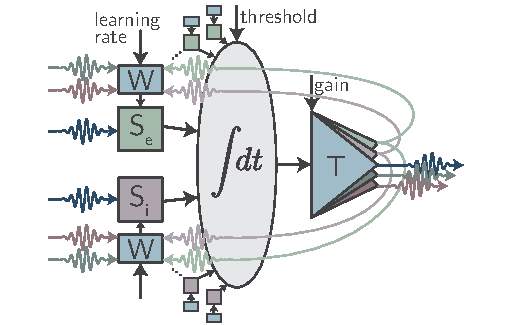
\includegraphics[width=8.6cm]{_general_schematic_small.pdf}}
	\caption{\label{fig:general_schematic}Schematic diagram of a loop neuron showing excitatory ($\mathsf{S_e}$) and inhibitory ($\mathsf{S_i}$) synapses, as well as synaptic weight update circuits ($\mathsf{W}$). The wavy, colored arrows are photons, and the straight, black arrows are electrical signals. The synapses receive signals as faint as a single photon and add supercurrent to an integration loop. Upon reaching threshold, a signal is sent to the transmitter circuit ($\mathsf{T}$), which produces a photon pulse. Some photons from the pulse are sent to downstream synaptic connections, while some are used locally to update synaptic weights.}
\end{figure}
We refer to relaxation oscillators sending few-photon signals that are received with superconducting detectors as superconducting optoelectronic neurons. In the specific neurons studied in this work, integration, synaptic plasticity, and dendritic processing are implemented with inductively coupled loops of supercurrent. We therefore refer to devices of this type as loop neurons. The loop neuron presented in this paper is shown schematically in Fig.\,\ref{fig:general_schematic}. A full circuit diagram is shown in Fig. \ref{fig:transmitters_fullCircuit}. The remainder of this section is an overview of the circuits described in more detail in the rest of the paper. Operation of loop neurons is summarized as follows. 

Photons from upstream neurons are received by superconducting SPDs at a neuron's synapses. Using Josephson circuits, these detection events are converted into an integrated supercurrent which is stored in a loop. The amount of current that gets added to the integration loop during a photon detection event is determined by the synaptic weight. The synaptic weight is dynamically adjusted by another circuit combining SPDs and JJs. When the integrated current of a given neuron reaches a (dynamically variable) threshold, an amplification cascade begins, resulting in the production of light from a waveguide-integrated semiconductor light emitter. The photons thus produced fan out through a network of dielectric waveguides and arrive at the synaptic terminals of other neurons where the process repeats.

In these loop neurons, a synapse consists of an SPD in parallel with a JJ (which together transduce photons to supercurrent), and a superconducting loop, which stores a current proportional to the number of detected photon arrival events. This loop is referred to as the synaptic integration (SI) loop. Within each neuron, the loops of many synapses are inductively coupled to a larger superconducting loop, referred to as the neuronal integration (NI) loop, thereby inducing an integrated current proportional to the current in all the neuron's synapses. When the current in this NI loop reaches a threshold, the neuron produces a current pulse in the form of a flux quantum. This current is amplified and converted to voltage to produce photons from a semiconductor $p-i-n$ junction.

The currents in the synaptic and neuronal integration loops are analogous to the membrane potential of biological neurons \cite{daab2001}, and the states of flux in these loops are the principal dynamical variables of the synapses and neurons in the system. Inhibitory synapses can be achieved through mutual inductors with the opposite sign of coupling. Dendritic processing can be implemented straightforwardly by adding intermediate mutually inductively coupled loops between the synaptic and neuronal loops. Synapses can be grouped on dendritic loops capable of local, nonlinear processing and inhibition \cite{sase2001,bu2006,robu2015}. Dendrites capable of detecting specific sequences of synaptic firing events \cite{thde2001,haah2015} can also be achieved. Neurons with multiple levels of dendritic hierarchy can be implemented as multiple stages of integrating loops. Clustering synapses on multiple levels of hierarchy in this way enables information access at gradually larger length scales across the network through transient synchronization at gradually lower frequencies \cite{stsa2000}. The temporal scales of the loops can be set with $L/r$ time constants, so different components can operate on different temporal scales, enabling relaxation oscillators with rich temporal dynamics. These relaxation oscillators can be combined in networks with dynamic functional connectivity, reconfigurable through inhibition and synaptic plasticity \cite{robu2015,fr2015}. These receiver circuits and integration loops are presented in Sec.\,\ref{sec:receiverCircuits}.

Synaptic memory is also implemented based on the stored flux in a loop, referred to as the synaptic storage (SS) loop. The state of flux in the SS loop determines the current bias to the synaptic receiver circuit discussed above. This current bias is the synaptic weight. If the SS loop is created with a superconducting wire of high inductance, the loop can hold many discrete states of flux, and therefore can implement many synaptic weights. In Sec.\,\ref{sec:synapticPlasticity} we investigate synapses with a pseudo-continuum of hundreds of stable synaptic levels between minimal and maximal saturation values, and we show that transitions between these levels can be induced based on the relative arrival times of photons from the pre-synaptic and post-synaptic neurons, thereby establishing a means for spike-timing-dependent plasticity with one photon required for each step of the memory update process. 

While synapses with many stable levels are advantageous to extending memory retention times \cite{fuab2007}, it is also important to implement synapses that change not only their efficacy based on pre- and post-synaptic spike timing, but also change their probability of changing their efficacy \cite{fudr2005}. Just as the synaptic weight is adjusted through a current bias on the receiver circuit, the probability of changing the synaptic weight can be adjusted through a current bias on the synaptic update circuit. As in the dendrites, we see a hierarchy can be achieved. In the case of synaptic memory, the synaptic weight and its rates of change are implemented in a loop hierarchy, and the state of flux in the loops can be dynamically modified based on photons generated by neural activity. Similar mechanisms can be utilized to adjust the synaptic weight based on short-term activity from the pre-synaptic neuron \cite{abre2004} or on a slowly varying temporal average of post-synaptic activity \cite{bico1982,cobe2012}. The synaptic memory circuits we develop in Sec.\,\ref{sec:synapticPlasticity} are logical extensions of binary memory cells utilized in superconducting digital electronics \cite{vatu1998,ka1999}.

The aspect of superconducting optoelectronic neuron operation that is most difficult to achieve is the production of light. The superconducting electronic circuits that perform the aforementioned synaptic and neuronal operations operate at millivolt levels, whereas production of the near-infrared photons desirable for communication requires a volt across a semiconductor diode. When a neuron reaches threshold, an amplification sequence begins. Current amplification is first performed, and the resulting large supercurrent is used to induce a superconducting-to-normal phase transition in a length of wire. When the current-biased wire becomes resistive, a voltage is produced via Ohm's law. This device leverages the extreme nonlinearity of the quantum phase transition to quickly produce a large voltage and an optical pulse. These transmitter circuits are discussed in Sec.\,\ref{sec:transmitterCircuits}.

The photons of a neuronal pulse are distributed over a large axonal network of passive dielectric waveguides. These waveguides terminate at each of the downstream synaptic connections. A downstream synaptic firing event will occur with near-unity probability at any connection receiving one or more photons. Photons of multiple colors can be generated simultaneously or independently, and different colors can share routing waveguides, while being used for different functions on the receiving end, such as synaptic firing and synaptic update. The number of photons produced during a neuronal firing event is the gain of the neuron, and the gain can be manipulated with the current bias to the light emitter. The network of waveguides that routes the communication events is discussed in Sec.\,\ref{sec:networks}.

To make the analogy to biological neural hardware explicit, synapses are manifest as circuits comprising superconducting SPDs with JJs. These synapses transduce photonic communication signals to supercurrent for information processing, and this supercurrent plays the role of the membrane potential. The dendritic arbor is a spatial distribution of synapses interconnected with inductively coupled loops for intermediate integration and nonlinear processing. The integration function of the soma is also achieved with a superconducting loop, and the threshold is detected when a JJ in this loop is driven above its critical current. The firing function of the soma (or axon hillock) is carried out by a chain of superconducting current and voltage amplifiers that drive a semiconductor diode to produce light. The axonal arbor is manifest as dielectric waveguides that route photonic signals to downstream synaptic connections. Gap junctions may be realized with evanescent couplers between waveguides of the axonal arbor, but we do not consider gap junctions further in this paper.

\subsubsection{\label{sec:implementation}Implementation}
Loop neurons combine several core devices: superconducting single-photon detectors \cite{gook2001,nata2012,liyo2013,mave2013}, Josephson junctions \cite{ti1996,vatu1998,ka1999}, superconducting mutual inductors \cite{miha2005}, superconducting current \cite{mcbe2014,mcab2016} and voltage amplifiers \cite{zhto2018}, semiconductor light sources \cite{shbu2017,buch2017}, and passive dielectric waveguide routing networks \cite{chbu2017,sami2017,chbu2018}. While all the components of these neurons have been demonstrated independently, their combined operation has not been shown. The experimental effort to achieve circuit integration is underway. Yet the physical principles of their operation and the designs presented in this paper indicate the potential for loop neurons to achieve complex, large-scale systems. The straightforward implementation of inhibition; the realization of a variety of temporal scales through $L/r$ time constants; single-photon-induced synaptic plasticity; and dynamically variable learning rate, threshold, and gain indicate these relaxation oscillators are promising as computational primitives. In conjunction with dense local and fast distant communication over passive waveguides, the system appears capable of the spatial and temporal information integration necessary for cognition and binding. 
	
We do not propose superconducting optoelectronic networks (SOENs) as an alternative to established neural hardware, but rather as a symbiotic technology. The success of neural CMOS (including optical communication above a certain spatial scale) will contribute to the success of SOENs, as it will be advantageous for SOENs to interface with CMOS via photonic signaling over fiber optic links between cryogenic and ambient environments. SOEN hardware is particularly well suited to interfacing with other cryogenic technologies such as imaging systems with superconducting sensors  \cite{alve2015,chsc2017}, as are commonly employed for medical diagnostics \cite{hada2016}, exoplanet search \cite{raca2016,boga1992,kila2016}, cosmology \cite{diad2017}, and particle detectors \cite{le2017}. Another intriguing application is in conjunction with other advanced computing technologies such as flux-based logic \cite{li2012,taoz2013,hehe2011} and quantum computers \cite{nich2000,blga2007,Zwanenburg2013,Hill,we2017}. One can envision a hybrid computational platform \cite{deli2017,posc2017} wherein a quantum module utilizes entanglement and superposition, while a neural module performs quantum-limited measurements and learns the behavior of the quantum system, and classical fluxon logic controls the operation of both. A superconducting optoelectronic hardware platform is likely to satisfy the computation and communication requirements of this hybrid technology. 

At this point we have described the motivations for loop neurons, and we have summarized their operation. The remainder of the document contains technical details of circuit operations (Secs.\,\ref{sec:receiverCircuits}-\ref{sec:transmitterCircuits}) and scaling analysis (Sec.\,\ref{sec:networks}).

%--------------------------------------------------
%receiver circuits
%--------------------------------------------------
\section{\label{sec:receiverCircuits}Synaptic Receiver Circuits}
The focus of this section is on the conversion of photonic communication events on many synapses to an integrated total signal stored in the neuron. These optoelectronic devices must meet several criteria: 1) the neuron must be able to achieve leaky integrate-and-fire functionality \cite{daab2001,geki2002} wherein activity on multiple synapses contributes to an integrated signal with a controllable leak rate; 2) single-photon detection events must contribute to the integrated signal, and the amount each detection event contributes to the integrated signal should depend on a dynamically reconfigurable synaptic weight; 3) neurons that are sensitive to the sum of spike events must be achievable in order to make use of rate-coded signals \cite{st1967}, and neurons that are sensitive to the timing between afferent spikes must also be achievable in order to make use of temporal coding \cite{thde2001,geki2002,sase2001,stgo2005}; 4) the circuits must scale to thousands of synaptic connections to integrate information across moderately sized cognitive circuits\,\footnote{Information integration in neural systems requires a short average path length across the network. Achieving a short average path length requires each node to form a large number of connections. For example, in a random network with one million nodes, each node must have one thousand connections to maintain an average path length of two. This subject is discussed in more detail in Ref.\,\onlinecite{sh2018_ICRC}.}; 5) the dynamic range of the neuron and synapses should allow activity on a large fraction of the synapses to contribute to a neuronal firing event, yet repeated activity on a small fraction of the synapses should also be able to induce a neuronal firing event; 6) synapses with inhibitory as well as excitatory functionality must be achievable, and inhibition must work in conjunction with dendrites \cite{budr2004,bu2006,haah2015} to enable synchronization on multiple time scales \cite{sase2001,enfr2001,vala2001,budr2004,robu2015}. This section explores circuit designs satisfying these criteria. 
	
\subsection{\label{sec:circuitOperation}Circuit operation}
\begin{figure}[t!]
	\centerline{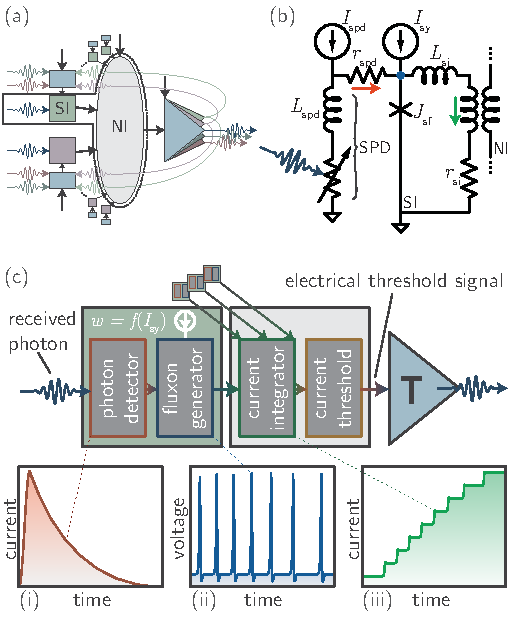
\includegraphics[width=8.6cm]{_receivers_schematic_small.pdf}}
	\caption{\label{fig:receivers_schematic}(a) Schematic of the neuron, as shown in Fig.\,\ref{fig:general_schematic}. Here, the dashed line encloses the synaptic receiver and neuronal integration loop that we describe in this section. (b) Circuit diagram of a simple photon-to-fluxon transducer combining a single-photon detector, Josephson junction, and flux storage loop. (c) Sequence of events during synaptic firing event. (i) Single-photon detector transduces photon to electrical current. (ii) Fluxons produced when SPD diverts current to JJ. The number of fluxons is determined by the synaptic bias current, which is controlled by the box labeled $\mathsf{W}$ in (a), discussed in Ref.\,\onlinecite{sh2018c}. (iii) Fluxons added to integration supercurrent storage loop. When the current in the loop reaches threshold, an electrical signal is sent to the transmitter.}
\end{figure}
The synaptic receiver is enclosed within the dashed boundary of Fig.\,\ref{fig:receivers_schematic}(a). A simple instantiation of the synaptic circuit is shown in Fig.\,\ref{fig:receivers_schematic}(b), and the operation of the synapse illustrated schematically in Fig.\,\ref{fig:receivers_schematic}(c). This receiver circuit in the context of the other components of the neural circuit is shown in Fig.\,\ref{fig:transmitters_fullCircuit} in Sec.\,\ref{sec:transmitterCircuits}. The synaptic receiver circuit comprises an SPD in parallel with a JJ embedded in a flux storage loop. This design is a reasonable starting point for a single-photon-sensitive synapse because it achieves transduction of a photonic signal to a superconducting electronic signal with a simple circuit. The design is similar to other superconducting particle detector circuits, such as transistion-edge bolometers \cite{vatu1998}. 

The operation of the synaptic circuit proceeds as follows. The SPD, shown as a variable resistor in series with an inductor in Fig.\,\ref{fig:receivers_schematic}(b), has zero resistance in the steady state, and it switches to a high-resistance state temporarily upon absorption of a photon. When a photon is detected, an electrical current is diverted from the SPD to a JJ, referred to as the synaptic firing junction ($J_{\mathrm{sf}}$). The current diverted from the SPD (Fig.\,\ref{fig:receivers_schematic}(c) part (i)) causes the net current through $J_{\mathrm{sf}}$ to exceed $I_{\mathrm{c}}$, generating a series of fluxons (Fig.\,\ref{fig:receivers_schematic}(c) part (ii)). We refer to this detection of a photon by the SPD and subsequent generation of fluxons by the JJ as a synaptic firing event. The synaptic weight of the connection is implemented via the current bias across $J_{\mathrm{sf}}$. The effect of this synaptic weight is to change the duration the JJ bias current exceeds $I_{\mathrm{c}}$, and therefore the number of fluxons generated during a synaptic firing event. If the synaptic weight is weak, a small number of fluxons, and therefore a small total amount of supercurrent, will be generated. If the synaptic weight is strong, a large number of fluxons, and therefore a large amount of supercurrent, will be generated during the synaptic firing event. The SPD response is virtually identical whether the number of photons present is one or greater than one, and for energy efficiency it is advantageous to send the fewest number of photons possible to each synaptic connection. The SPD response also does not depend strongly on the frequency of light across a bandwidth broad enough for multiplexing \cite{mave2013}. Implementing synaptic weight in the electronic domain in this manner makes use of both the speed and energy efficiency of JJs, while leveraging the strengths of light for communication.  

The supercurrent generated during each synaptic firing event is added to a superconducting loop, called the synaptic integration (SI) loop, which integrates the total current from all synaptic firing events at that synapse (Fig.\,\ref{fig:receivers_schematic}(c) part (iii)). Many synapses will be coupled to a larger neuronal integration (NI) loop via mutual inductors. The NI loop combines the signals from all the synapses connected to the neuron. Ultimately, the current coupled to the NI loop is increased using a current transformer which induces current in a final loop, the neuronal thresholding (NT) loop. The NT loop is a superconducting loop which contains a JJ ($J_{\mathrm{nf}}$) that produces an output current pulse when its critical current (threshold) is reached \cite{crsc2010}. This threshold can be dynamically varied with a current bias. The current pulse generated when the neuron reaches threshold is amplified and ultimately used to trigger a photon\textendash generation event.

The number of flux quanta generated in a synaptic firing event depends on the relation between $I_{\mathrm{c}}$, $I_{\mathrm{spd}}$, and $I_{\mathrm{sy}}$, as well as the SPD time constant, $L_{\mathrm{spd}}/r_{\mathrm{spd}}$. If the bias current $I$ is close to but greater than $I_{\mathrm{c}}$, the time-averaged voltage across the junction will be given by $\langle V \rangle \approx R \sqrt{I^2-I_c^2}$, where $R$ is the junction resistance in the non-superconducting state. The rate of generation of flux quanta is given by $r_{\mathrm{sfq}} = \langle V \rangle/\Phi_0$ \cite{ka1999}. This generated flux is trapped in the SI loop. Utilization of a JJ in this circuit is advantageous to decouple the amount of current added to the loop from the time it is stored in the loop. The current in each SI loop decays with the $\tau_{\mathrm{si}} = L_{\mathrm{si}}/r_{\mathrm{si}}$ time constant, which can be chosen over a broad range. By choosing $\tau_{\mathrm{si}}$ to be different for different synapses, one can diversify the temporal information provided to the neuron \cite{stsa2000,abre2004,budr2004,be2007}.

The circuit of Fig.\,\ref{fig:receivers_schematic}(b) captures the concept of the receiver, but its performance is limited in this configuration because the SI loop saturates at a small current. Higher saturation current is achieved by separating the transduction operation from the SI loop by a Josephson transmission line (JTL) \cite{ka1999,vatu1998}, as shown in Fig.\,\ref{fig:receivers_circuitDiagrams}(a). This form of the receiver circuit is the form used as a synapse in this work. 
\begin{figure}[t!]
	\centerline{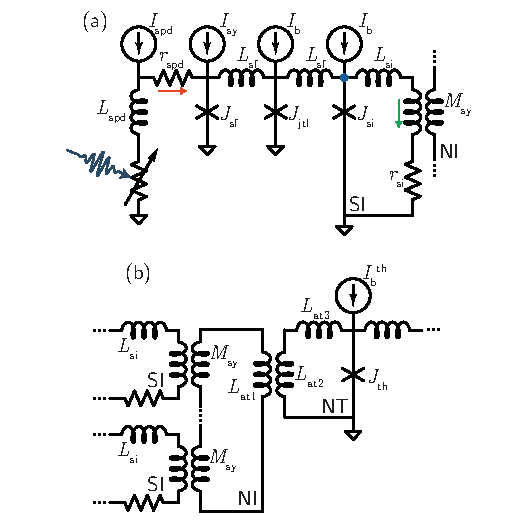
\includegraphics[width=8.6cm]{_receivers_circuitDiagrams_small.pdf}}
	\caption{\label{fig:receivers_circuitDiagrams}(a) Circuit diagram of the photon-to-fluxon transducer connected to the synaptic integration loop by a JTL. (b) Circuit diagram of multiple synapses connected to the neuronal integration loop and the neuronal thresholding loop.}
\end{figure}

In the configuration of Fig.\,\ref{fig:receivers_circuitDiagrams}(a), the fluxons produced by the switching of $J_{\mathrm{sf}}$ during a synaptic firing event propagate down a JTL (a single JJ in this study), and drive the switching of a junction inside the SI loop.
\begin{figure}[t!]
	\centerline{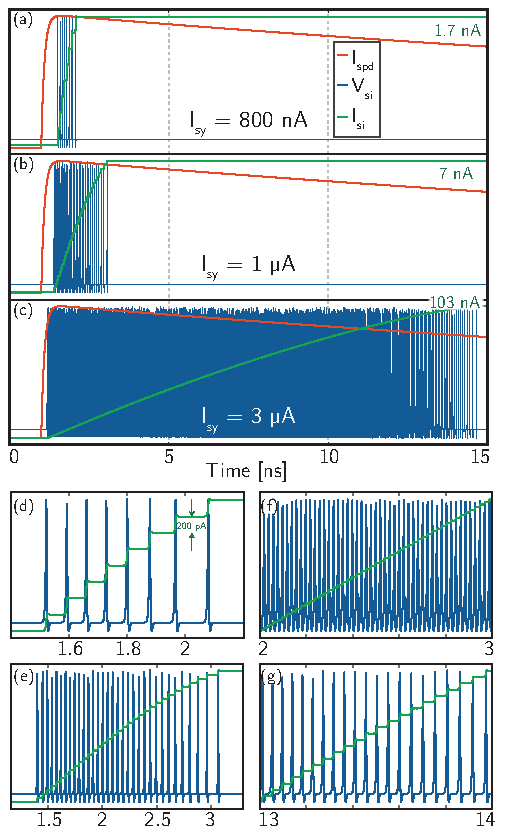
\includegraphics[width=8.6cm]{_receivers_sffg_firingDetail_small.pdf}}
	\caption{\label{fig:receivers_sffg_firingDetail} Operation of the synaptic firing circuit during a synaptic firing event for three values of $I_{\mathrm{sy}}$. The three traces in each of these plots are normalized such that the maximum of each trace within the displayed time window is set to one and the minimum is set to zero. The colors of the traces are in reference to the current paths and voltage node labeled in Fig.\,\ref{fig:receivers_circuitDiagrams}(a). (a) Activity of the synaptic firing circuit for $I_{\mathrm{sy}} = 800$\,nA. (b) Activity of the synaptic firing circuit for $I_{\mathrm{sy}} = 1$\,\textmu A. (c) Activity of the synaptic firing circuit for $I_{\mathrm{sy}} = 3$\,\textmu A. (d) Temporal zoom for $I_{\mathrm{sy}} = 800$\,nA. (e) Temporal zoom for $I_{\mathrm{sy}} = 1$\,\textmu A. (f) Temporal zoom near the beginning of the photon-detection pulse for $I_{\mathrm{sy}} = 3$\,\textmu A. (g) Temporal zoom near the end of the photon-detection pulse for $I_{\mathrm{sy}} = 3$\,\textmu A.} 
\end{figure}  
The fluxons from multiple synaptic firing events can be stored in the SI loop, and therefore we may wish to use a loop that can contain many fluxons. The current added to the loop by a single fluxon is $I_{\phi} = \Phi_0/L_{\mathrm{si}}$, where $\Phi_{0} = h/2e = 2.07\times 10^{-15}$\,Wb is the magnetic flux quantum. The SI loop can maintain a linear response in the presence of many synaptic firing events if $L_{\mathrm{si}}$ is chosen to be large, or the SI loop can saturate if $L_{\mathrm{si}}$ is chosen to be small, thus providing one means of implementing short-term plasticity \cite{abre2004,sh2018c}.

The SI loops are inductively coupled to the NI loop, (Fig.\,\ref{fig:receivers_circuitDiagrams}(b)), which stores a current proportional to the sum of the currents in all the SI loops. The use of mutual inductors allows many synapses to add current to an NI loop without introducing leakage current pathways. Finally, the NI loop couples to a third loop, the NT loop. The mutual inductor coupling the NI loop to the NT loop serves as a transformer to step up the current to be detected at threshold. The NT loop may not need to be a separate loop when the number of synapses, $N_{\mathrm{sy}}$, is small. The performance of the NT loop upon reaching current threshold is discussed in Sec.\,\ref{sec:transmitterCircuits}.

In Fig.\,\ref{fig:receivers_sffg_firingDetail}, we simulate the operation of the synaptic receiver as it experiences a synaptic firing event. We use WRSpice \cite{wh1991} to model the circuit of Fig.\,\ref{fig:receivers_circuitDiagrams}(a). We treat the SPD as a current source with exponential rise with 100 ps time constant followed by exponential decay with 50 ns time constant. The amplitude of the SPD current pulse is 10\,\textmu A. All circuit parameters used in this work are given in Appendix \ref{apx:circuitParameters}. Figures \ref{fig:receivers_sffg_firingDetail}(a)-(c) show the activity of a synaptic firing event for $I_{\mathrm{sy}} = 800$\,nA, 1\,\textmu A, and 3\,\textmu A. With $I_{\mathrm{sy}} = 800$\,nA, the junction is briefly driven above $I_{\mathrm{c}}$, and eight fluxons are transmitted to the SI loop. The synaptic firing event causes the current in the SI loop, $I_{\mathrm{si}}$, to increase by 1.7\,nA. If we increase the bias current to $I_{\mathrm{sy}} = 1$\,\textmu A, the synaptic firing event produces 33 fluxons and adds 7\,nA to the SI loop. Further increasing the synaptic bias to 3\,\textmu A gives the behavior shown in Fig.\,\ref{fig:receivers_sffg_firingDetail}(c). In this case, 497 fluxons add 103\,nA to the SI loop. The period of the voltage pulses is observed to decrease through the duration of the SPD pulse, demonstrating the decrease of $r_{\mathrm{sfq}}$ as current returns to the SPD and the net bias across the JJ decays, as discussed above. Details of synaptic firing are shown in Fig.\,\ref{fig:receivers_sffg_firingDetail}(d)-(g). The energy consumed by a synaptic firing event is discussed in Appendix \ref{sec:appendix_energy}.

The analysis of Fig.\,\ref{fig:receivers_sffg_firingDetail} gives the currents and voltages present during a synaptic firing event for three values of $I_{\mathrm{sy}}$. Systematic analysis of $I_{\mathrm{si}}$ versus $I_{\mathrm{sy}}$ finds a quadratic trend. A principal objective of this analysis is to determine the range of synaptic bias currents over which we would like to operate. Operating with a minimum synaptic bias of 1\,\textmu A enables us to work close to the energy-efficiency limit of the circuit, and we anticipate that the exact number of fluxons produced during a firing event will be noisy, much like the activity of a biological neuron \cite{stgo2005}. The amount of current added to the SI loop during a synaptic firing event with strong synaptic weight should be significantly larger than the amount of current with a weak synaptic weight. We choose $I_{\mathrm{sy}} = 3$\,\textmu A to be the largest synaptic bias at which we would like to operate, and thus a synaptic firing event with a strong synaptic bias adds 15 times as much current to the SI loop (and therefore the NI loop and NT loop) as a firing event with a weak synaptic bias. This ratio is entirely tunable based on the needs of the system. Learning\textemdash either supervised or unsupervised \textemdash should adjust the synaptic bias current over the range 1\,\textmu A $< I_{\mathrm{sy}} < 3$\,\textmu A for the parameters considered here. Circuits accomplishing this are discussed in Sec.\,\ref{sec:synapticPlasticity}.

\subsection{\label{sec:scaling}Multisynaptic neurons}
In general, a neuron will combine signals from many synaptic connections and produce a pulse when this combined signal reaches a threshold. We would like to know how devices will perform when many synapses are integrated with a single NI loop. We find that the SI loop with the design described above can receive over 1000 synaptic firing events when $I_{\mathrm{sy}} = 1$\,\textmu A, and 82 synaptic firing events when $I_{\mathrm{sy}} = 3$\,\textmu A before saturation of the loop occurs (assuming $\tau_{\mathrm{si}}\rightarrow \infty$). If the loop contains a resistance, the trapped flux will leak with the $L/r$ time constant, leaving the synapse ready to receive further synaptic firing events. 

We wish to know how inductively coupling multiple SI loops to a single NI loop affects the operation during synaptic firing events. WRSpice simulations show that a synaptic firing event of a neuron with a single synaptic connection and a synaptic firing event of a single synapse connected to an NI loop with 10 synaptic connections produce an identical number of fluxons with identical timing. The effect of timing delay between two synaptic firing events on different synapses in a neuron of $N_{\mathrm{sy}} = 10$ has also been considered. The total current added to the NI loop is independent of the timing delay between the two synaptic firing events. These linearities with respect to $N_{\mathrm{sy}}$ and pulse timing delay are attractive features of inductively coupled synapses. Contexts in which nonlinearity with respect to arrival time is desirable, such as for temporal coding \cite{thde2001,sase2001} or dendritic processing \cite{brcl2010,haah2015}, are likely to employ two-photon receiver circuits such as discussed in Sec.\,\ref{sec:dendriticProcessing}. Implementing SI loops with inductive coupling to an NI loop enables scaling to neurons with many synapses without cross talk or unwanted nonlinearities related to timing.
 
\begin{figure}[t!]
	\centerline{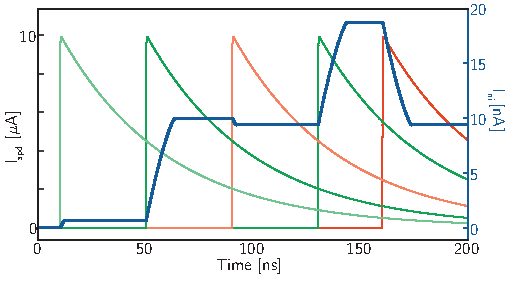
\includegraphics[width=8.6cm]{_receivers_inhibitoryAndExcitatory_small.pdf}}
	\caption{\label{fig:receivers_inhibitoryAndExcitatory}A neuron with seven excitatory and three inhibitory synaptic connections. The excitatory and inhibitory current inputs are shown as green and red traces and are referenced to the left $y$ axis. The blue trace is $I_{\mathrm{sy}}$, referenced to the right $y$ axis. At time $t = 10$ ns, a synaptic firing event occurs on an excitatory synapse with $I_{\mathrm{sy}} = 1$\,\textmu A. At time $t = 50$\,ns, a synaptic firing event occurs on an excitatory synapse with $I_{\mathrm{sy}} = 3$\,\textmu A. At time $t = 90$\,ns, a synaptic firing event occurs on an inhibitory synapse with $I_{\mathrm{sy}} = 1$\,\textmu A. At time $t = 130$\,ns, a synaptic firing event occurs on an excitatory synapse with $I_{\mathrm{sy}} = 3$\,\textmu A. At time $t = 160$\,ns, a synaptic firing event occurs on an inhibitory synapse with $I_{\mathrm{sy}} = 3$\,\textmu A. The colors in this plot are not in reference to Fig.\,\ref{fig:receivers_circuitDiagrams}.}
\end{figure}
It is important for a neuron to be able to receive excitatory and inhibitory connections \cite{vrso1996,sase2000,daab2001,robu2015}. Inhibitory connections keep the network from experiencing runaway activity and are crucial for temporal synchronization \cite{sase2001,vala2001,enfr2001,budr2004,bu2006}. Inhibitory connections can be constructed with the same photon-to-fluxon transduction circuit presented thus far by changing the sign of $M_{\mathrm{sy}}$. We investigate a neuron with seven excitatory and three inhibitory connections in Fig.\,\ref{fig:receivers_inhibitoryAndExcitatory}. The figure shows a time trace of $I_{\mathrm{ni}}$ as three excitatory and two inhibitory synaptic firing events occur. An excitatory event and an inhibitory event occur in synapses with $I_{\mathrm{sy}} = 1$\,\textmu A, and the other events occur in synapses with $I_{\mathrm{sy}} = 3$\,\textmu A. This plot demonstrates the dynamic state of a multi-synaptic neuron under the influence of excitation and inhibition. 

The symmetry between inhibitory and excitatory synapses is broken by $I_{\mathrm{b}}^{\mathrm{th}}$, the current bias across the thresholding junction. The circuit can be designed so saturation of all inhibitory SI loops is insufficient to add enough counter current to the NT loop to overcome  $I_{\mathrm{b}}^{\mathrm{th}}$ and reach threshold. Thus, repeated excitatory events can drive the neuron to spike, but repeated inhibitory events can only move the device further from threshold and cannot trigger a spike, much like the polarizing effects of inhibitory interneurons in biological neural systems.
	
\subsection{\label{sec:dendriticProcessing}Dendritic processing}
In addition to neurons that integrate single-photon pulses, as described in Sec. \ref{sec:circuitOperation}, it is desirable to achieve neurons that detect coincident signals from two or more pre-synaptic neurons for detecting temporally coded information \cite{thde2001,sase2001,stse2007,sp2008,brcl2010,haah2015}. The mutual information regarding a stimulus conveyed by two or more neurons can be approximated by a Volterra expansion \cite{geki2002} with the leading term corresponding to firing rate, and the second-order term representing correlations \cite{pasc1999}. In biological neurons, temporal synaptic sequences can be detected using hardware nonlinearities present in dendrites \cite{brcl2010,haah2015}, which perform important cortical computations. Detection of timing correlations and sequences can be achieved in optoelectronic hardware using two (or more) SPDs in a similar circuit to the synaptic receiver of Fig.\,\ref{fig:receivers_circuitDiagrams}(a). 

In Fig.\,\ref{fig:receivers_coincidence} we analyze a two-photon symmetrical coincidence detection circuit. The circuit diagram is shown in Fig.\,\ref{fig:receivers_coincidence}(a). The two SPDs are biased symmetrically, and the circuit is designed such that if either SPD detects a photon in isolation, the current across $J_{\mathrm{sf}}$ remains below $I_{\mathrm{c}}$, but if both detect a photon within a certain time window, the current across $J_{\mathrm{sf}}$ can exceed $I_{\mathrm{c}}$, adding current to the SI loop. The amount of current added to the SI loop is plotted as a function of the difference in arrival times between two photons in Fig.\,\ref{fig:receivers_coincidence}(b). WRSpice was again used for these simulations, but in this case the SPDs were modeled not as current sources, but as resistors of 5\,k$\Omega$ with 200\,ps duration occurring at specified photon-arrival times \cite{yake2007}. The time scale over which correlated events are detected is set by the $L_{\mathrm{spd}}/r_{\mathrm{spd}}$ time constant of the circuit. In the main panel, this time constant is 500\,ns, and in the inset it is 50\,ns. Longer correlation windows can be straightforwardly achieved, and the shortest correlation window will be limited by the latching time of the SPDs.
\begin{figure}[t!]
	\centerline{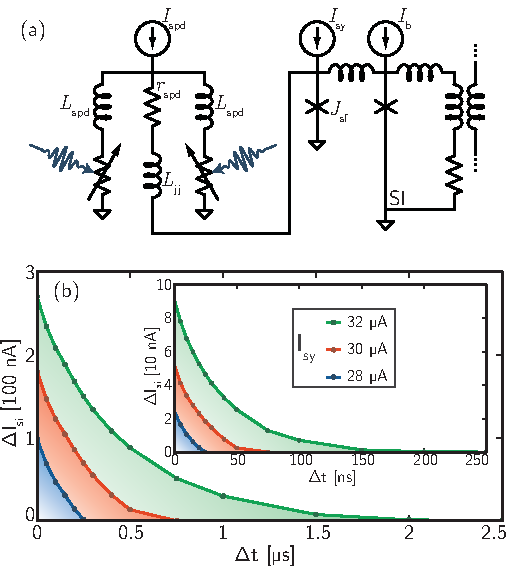
\includegraphics[width=8.6cm]{_receivers_coincidence_small.pdf}}
	\caption{\label{fig:receivers_coincidence}Coincidence-detection circuit for neurons sensitive to temporal coding. (a) Circuit diagram of symmetric two-photon coincidence detection circuit. (b) Current added to SI loop as a function of time delay between arrival of the photons. Performance was calculated for the three values of $I_{\mathrm{sy}}$ shown in the legend. Circuit parameters are given in Appendix \ref{apx:circuitParameters}.}
\end{figure}

Due to the symmetric biasing of the two SPDs, the circuit of Fig.\,\ref{fig:receivers_coincidence} is insensitive to order of photon arrival. By breaking this symmetry, similar receiver circuits that detect ordered correlations can be used for Hebbian learning. The two-SPD circuit of Fig.\,\ref{fig:receivers_coincidence} can also be extended to detect other sequences of activity, including sequences with more photons. 
\begin{figure}[t!]
	\centerline{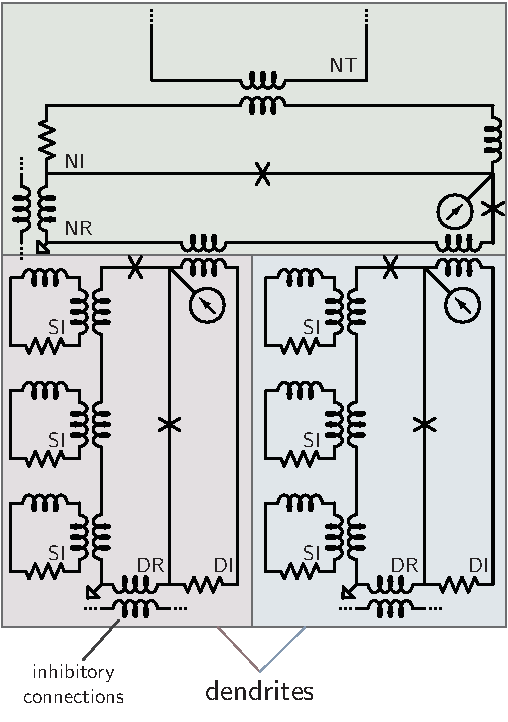
\includegraphics[width=8.6cm]{_receivers_dendriticProcessing_small.pdf}}
	\caption{\label{fig:receivers_dendriticProcessing} Dendritic processing with loops. Schematic of two-level loop hierarchy for nonlinear electrical response.}
\end{figure}

Dendritic processing can also be used for intermediate nonlinear processing between synapses and the NI loop \cite{sava2017}. An example circuit is shown in Fig.\,\ref{fig:receivers_dendriticProcessing}. Here, multiple SI loops are inductively coupled to another loop, which contains a JJ. Only when the junction is driven above its critical current does an appreciable signal get added to the dendritic integration (DI) loop, which is an intermediate, nonlinear processor between the SI loops and the NI loop. In this case, the DI loops are analogous to dendrites. An important role of dendrites is in conjunction with inhibitory interneurons that can temporarily suppress the efficacy of an entire dendrite \cite{budr2004,bu2006,robu2015}. At the bottom of Fig.\,\ref{fig:receivers_dendriticProcessing} we show how an inhibitory interneuron may be inductively coupled to a dendrite. When inhibition is applied to the loop, it may be impossible for the synaptic connections to drive the JJ above threshold and add flux to the DI loop. Many levels of loop hierarchies can be combined in this way to achieve various nonlinear functions as well as current amplification before the NT loop.

Dendritic processing in conjunction with inhibitory interneurons contributes to network synchronization on various temporal and spatial scales \cite{vala2001,enfr2001,sase2001,bu2006,buwa2012,robu2015}. The approach to dendrites shown in Fig.\,\ref{fig:receivers_dendriticProcessing} is one way inhibition could be used with the synapses presented here to achieve these functions thought to be necessary for cognition \cite{budr2004,fr2015}. In this context, engineering synaptic and dentritic circuits with a variety of time constants (analogous to membrane time constants) is important, as these time constants affect synchronization frequency \cite{lued1997} and enable neurons with a greater diversity of synapses \cite{ma2016}. As discussed in Sec.\,\ref{sec:introduction}, power-law dynamics are necessary for information integration and self-organized criticality, and a power-law frequency distribution can be achieved through the superposition of exponential decay functions with a diversity of time constants \cite{be2007}. To achieve this with the dendritic processors shown in Fig.\,\ref{fig:receivers_dendriticProcessing}, resistors are placed in each DI loop. The $L/r$ time constant of each DI loop will set its temporal response, and in this way, different dendrites can be given different time constants. Similarly, a resistor can be placed in each SI loop so that each synaptic excitation has a characteristic time constant, as discussed previously. These resistors will also accomplish the task of purging flux from the SI and DI loops to avoid saturation. As indicated in Fig.\,\ref{fig:receivers_dendriticProcessing}, inhibition can be applied at various points in the loop hierarchy, including specific synaptic loops, dendritic loops, the neuronal integration loop, and even the current source to the light emitter. These different structural implementations of inhibition are analogous to the three main forms of inhibition observed in biological neurons, wherein interneurons target dendrites, the soma, and the axon initial segment \cite{robu2015}.
	
\subsection{\label{sec:discussion_receiverCircuits}Discussion Regarding Synaptic Receiver Circuits}
The present section has investigated a superconducting optoelectronic neuron receiver circuit utilizing an analog photon-to-fluxon transducer, based on an SPD in parallel with a JJ, that couples flux to a storage loop. The synaptic weight can be enacted by changing the bias to the JJ. One thousand of these synapses can be inductively coupled to an integration loop and ultimately to a thresholding JJ. Designs for single-photon-sensitive receivers capable of operating on rate-coded signals as well as two-photon-sensitive receivers capable of operating on temporally coded signals have been discussed. Excitatory as well as inhibitory behavior has been simulated, and a hierarchy of loops for dendritic processing has been proposed.

In addition to utilization as a neural computer, experiments using these neural circuits may be useful for testing hypotheses in neuroscience. The circuits presented here can be reconfigured and extended to make use of numerous SPDs performing nonlinear correlation functions on signals from numerous pre-synaptic neurons as well as employing multiple integration loops, multiple thresholding elements, and multiple light sources suitable for experimenting with different synaptic and dendritic circuit paradigms. Additionally, similar receiver circuits can be utilized for dynamic learning, synaptic plasticity, and metaplasticity, as discussed in Sec.\,\ref{sec:synapticPlasticity}.

In Sec.\,\ref{sec:introduction} we argue that cognitive systems benefit from information integration across spatial and temporal scales. Temporal integration is achieved with a power-law distribution of neural oscillation frequencies. The receiver circuits presented in this work enable this functionality in at least two ways. First, they are fast and can detect photon communication events at 20 MHz and possibly faster. The brain oscillates at frequencies from 0.05\,Hz to 600\,Hz \cite{budr2004}. We assume loop neurons can oscillate from 1\,Hz to 20\,MHz, and the actual range may be larger. While the human brain oscillates at frequencies spanning four orders of magnitude, these receivers could contribute to oscillations across seven orders of magnitude or more, indicating the potential for information integration across very large networks \cite{stsa2000} (see Sec.\,\ref{sec:neuronalPool}). The second manner in which these receivers are well-suited to achieving a power-law frequency distribution is that their oscillatory response is tunable, so each neuron can participate in a broad range of oscillations. This tunable response is achievable by changing synaptic weights as well as the threshold of the JJ in the NI loop or DI loops via bias currents. Tunability also results from changing which synapses are effective at a given time using inhibition and dendritic processing. Such dynamic effects in synapses and neurons in the brain are crucial for maximally utilizing the time domain for information integration \cite{bu2006}.

Finally, we point out that while the circuits presented here utilize photons for communication and to trigger synaptic firing events, similar functionality is achievable using only fluxons. The SPD in Fig.\,\ref{fig:receivers_schematic}(b) can be replaced with an nTron \cite{mcbe2014}, the gate of which can be driven normal by one or more fluxons. The same techniques of utilizing a hierarchy of integration loops, dendritic processing, and synaptic weighting can be used in those circuits as well. Achieving the communication necessary for large networks \cite{sh2018_ICRC} will be cumbersome with purely electronic circuits. Yet such neurons may fire at rates beyond 10\,GHz with very low power consumption when driving up to $\approx$\,20 synaptic connections. Networks combining electronic and optoelectronic neurons extend the power-law degree distribution to lower degree and the power-law frequency distribution to higher frequency. Purely electronic, JJ-based neurons and synapses have been proposed \cite{hias2007,crsc2010,ru2016} and demonstrated \cite{segu2014,scdo2018}. We point out how the circuits presented here can be converted to purely electrical neurons to illustrate the continuity of electronic and photonic implementations, and to show that networks with both electrical and optical neurons working in conjunction based on the same neural principles and fabrication process can be achieved.

%%---------------------------------------------
%%synaptic plasticity
%%---------------------------------------------	
\section{\label{sec:synapticPlasticity}Synaptic Plasticity}
The synaptic weights between nodes of a neural system are crucial memory elements that affect dynamics and computation \cite{abre2004,bu2006,siqu2007,haah2015}. In the loop neurons under consideration, the photon-to-fluxon transduction that occurs during a synaptic firing event is implemented with an SPD in parallel with a JJ, as described in Sec.\,\ref{sec:receiverCircuits}. To change the number of fluxons generated during the synaptic firing event, one can simply change the current bias across $J_{\mathrm{sf}}$. The circuits presented in this section are designed to dynamically modify the current bias $I_{\mathrm{sy}}$ to $J_{\mathrm{sf}}$ (see Fig.\,2). We refer to the circuits that modify $I_{\mathrm{sy}}$ as synaptic update circuits.

In general, there will be a chosen weakest synaptic strength and strongest synaptic strength at each synapse, and in general the weakest synaptic strength may be achieved with $I_{\mathrm{sy}}^{\mathrm{min}} > 0$. Thus, it is the goal of a synaptic update circuit to vary $I_{\mathrm{sy}}$ over some range $I_{\mathrm{sy}}^{\mathrm{min}}\le I_{\mathrm{sy}} \le I_{\mathrm{sy}}^{\mathrm{max}}$. In certain contexts it is sufficient for $I_{\mathrm{sy}}$ to only be able to take two values  \cite{lide2015}, while in other learning environments it may be advantageous to access many values of $I_{\mathrm{sy}}$ between $I_{\mathrm{sy}}^{\mathrm{min}}$ and $I_{\mathrm{sy}}^{\mathrm{max}}$. In Sec.\,\ref{sec:receiverCircuits} we identified $I_{\mathrm{sy}}^{\mathrm{min}} = 1$\,\textmu A and $I_{\mathrm{sy}}^{\mathrm{max}} = 3$\,\textmu A. 

The circuits described in this section modify $I_{\mathrm{sy}}$ in either a supervised manner using JJs or unsupervised manner using SPDs in conjunction with JJs. For supervised operation, controlled inputs are presented to the system, and the system provides an output. The output from the system is compared to a desired output, and an error is calculated based on a cost function. This error is then used to update the configuration of the system, often through backpropagation \cite{ni2015}. The objective of supervised learning is usually to train the hardware to perform a specific task \cite{sihu2016}. 

For larger neural systems performing general cognitive functions, it is advantageous to operate in an unsupervised manner. Unsupervised learning often refers to the process of learning to categorize unlabeled data. Here, we use the term in a more general sense to refer to systems that learn without any supervisory control. In this modality, no outside entity modifies synaptic weights. Such an approach to learning is scalable in that a user is not required to calculate or adjust the network parameters, so systems with many more degrees of freedom can be realized. Unsupervised learning requires that internal activity of the network be capable of adjusting the degrees of freedom to form a useful representation of the information it is expected to process. This operation is achieved through a variety of activity-based plasticity mechanisms, including spike-timing-dependent plasticity (STDP).

For either supervised of unsupervised learning, the memory update signals add or remove flux from a storage loop, which is inductively coupled to $I_{\mathrm{sy}}$. This loop is referred to as the synaptic storage (SS) loop, and the flux stored in this loop functions as the memory for the synapse.
\begin{figure}[t!]
	\centerline{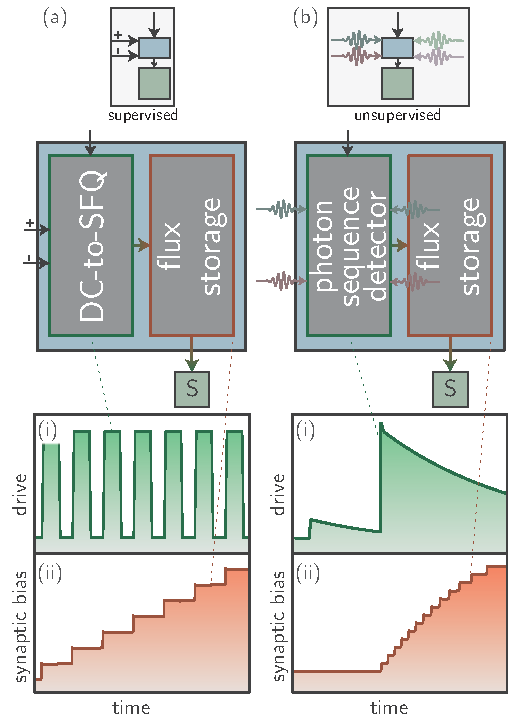
\includegraphics[width=8.6cm]{_synapticPlasticity_schematic_small.pdf}}
	\caption{\label{fig:synapticPlasticity_schematic}(a) Supervised synaptic weights. The top box references the schematic of Fig.\,\ref{fig:general_schematic}, and summary of operation is shown below. For supervised learning, input square pulses add or remove fluxons from a loop, which strengthens or weakens the synaptic weight. (b) Synaptic update in unsupervised mode. Photons from pre- and post-synaptic neurons update the weight by changing the flux in the SB loop.}
\end{figure}

For large-scale cognitive computing, we are interested in systems that will interact continuously with their environment, be capable of immediately assimilating new information, and also capable of remembering events as long as possible. Such competing memory demands are sometimes referred to as the adaptability-precision trade-off \cite{khso2017}, and the best-performing synapses in this regard are complex \cite{fudr2005} and may have many stable levels \cite{fuab2007}. In human subjects, memories have been observed to fade with a power-law temporal dependence \cite{wieb1991,wieb1997}. It is difficult to do better than power-law forgetting with plastic synapses that continually adapt \cite{fudr2005}, and simple synapses lose their memory trace most quickly \cite{fuab2007}. Here we show synapses with a number of stable states ranging from two to hundreds. These synapses have dynamically variable memory update rates, making the synapses suitable for power-law memory retention.

The circuits implemented to control $I_{\mathrm{sy}}$ must meet several criteria: 1) transition between the minimum and maximum values of $I_{\mathrm{sy}}$ should be possible with a specified number of increments to control the learning rate; 2) the circuit should not be able to set $I_{\mathrm{sy}}$ outside of this range so that simple update rules or training algorithms do not result in excessively large synaptic weights; 3) it should be possible to cycle the value of $I_{\mathrm{sy}}$ from minimum to maximum and back repeatedly without degradation; 4) in addition to a means by which the synaptic weights can be incremented by an external supervisor, there should be a means by which correlated photon signals from the two neurons associated with a synapse can strengthen or weaken the synaptic weight depending on the relative arrival times of the signals from the two neurons; 5) within this unsupervised mode of operation, synaptic update events should be induced by single-photon signals to fully exploit the energy efficiency of the superconducting optoelectronic hardware; 6) the transition probability between synaptic states should also be dynamically adjustable based on photonic signals to achieve metaplastic behavior. This section explores circuit designs satisfying these criteria.

Qualitative explanation of the memory update process in shown in Fig.\,\ref{fig:synapticPlasticity_schematic}(a) for supervised learning and in Fig.\,\ref{fig:synapticPlasticity_schematic}(b) for unsupervised learning. For the simplest supervised binary synapse, a flux-quantum memory cell can be used to switch between the strong and weak synaptic states in 50\,ps. This binary design can be extended to a multi-stable synapse that can modify the synaptic weight between the fully potentiated and fully depressed states with hundreds of stable intermediate levels, and implementations with more or less resolution are straightforward to achieve. For unsupervised learning, we consider a circuit that can implement a Hebbian learning rule that potentiates a synaptic connection using one photon from the pre-synaptic neuron and one photon from the post-synaptic neuron. We generalize this circuit to implement full STDP wherein a synaptic weight can be either potentiated or depressed based on Hebbian and anti-Hebbian timing correlations. This STDP circuit uses single-photon signals at four ports. Implementations of short-term plasticity, homeostatic plasticity, and metaplasticity are discussed in Ref.\,\onlinecite{sh2018c}. By combining these synaptic update circuits, it is possible to realize neurons with a distribution of synapses that update at different rates as well as ensembles of neurons wherein different neurons store information about different stimuli learned at different times, thus achieving a network with rapid adaptability and long memory retention times necessary for cognition. 
	
\subsection{\label{sec:supervised}Supervised learning}
At the present stage of development it is not clear which application spaces will be best served by superconducting optoelectronic hardware. The main emphasis of this work is on general cognitive systems, yet we begin the exploration of synaptic plasticity with supervised synapses to explore the possibilities and because the unsupervised circuits are straightforward extensions of these supervised circuits. To implement supervised learning, we would like to control the flux stored in the SS loop using simple control signals, which we take to be square current pulses. For many applications in machine learning, neural networks, and neuroscience, synapses are treated as binary elements that can switch between strong (potentiated) and weak (depressed) states \cite{amfu1994,fuab2007,lide2015}. In Sec.\,\ref{sec:receiverCircuits} it was shown that, in a superconducting optoelectronic loop neuron, changing $I_{\mathrm{sy}}$ from 1\,\textmu A to 3\,\textmu A changes the contribution to the neuron's integrated signal by a factor of 15. 
\begin{figure}[t!]
	\centerline{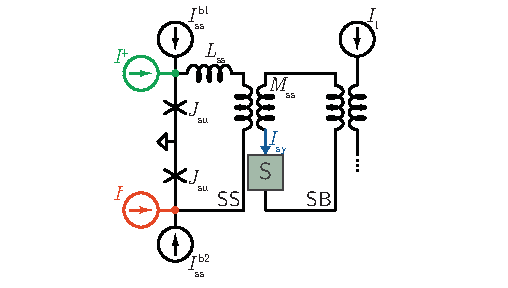
\includegraphics[width=8.6cm]{_synapticPlasticity_binaryCircuit_small.pdf}}
	\caption{\label{fig:synapticPlasticity_binaryCircuit}Fluxon memory cell used to achieve binary synapse. The box labeled $\mathsf{S}$ is the synapse receiving the bias current (see Fig.\,\ref{fig:synapticPlasticity_schematic}). Circuit parameters are listed in Appendix \ref{apx:circuitParameters}.}
\end{figure}
The circuit for enacting a binary synapse is shown in Fig.\,\ref{fig:synapticPlasticity_binaryCircuit}. For systems with many neurons each with many synapses, we would like to use a single current source to establish the baseline synaptic bias to all synapses ($I_1$ in Fig.\,\ref{fig:synapticPlasticity_binaryCircuit}), keeping in mind that we may need the baseline synaptic bias to be different for different synapses. This can be achieved by using a single current bias, $I_1$, and using mutual inductors to couple this current to each synapse. The synaptic firing circuit is thus biased by a superconducting loop, referred to as the synaptic bias (SB) loop, and the objective of the synaptic update circuit is to change the current in the SB loop, also through mutual inductors. This concept is shown in Fig.\,\ref{fig:synapticPlasticity_binaryCircuit}, where the SB loop is coupled to both the main bias, $I_1$, and the dynamic synaptic bias based on the flux trapped in the SS loop. All circuits presented in the remainder of this section provide a means to adjust the flux stored in the SS loop. 

The two-JJ circuit of Fig.\,\ref{fig:synapticPlasticity_binaryCircuit} is a standard flux-quantum memory cell \cite{ka1999,vatu1998} coupled to the SB loop via a mutual inductor \cite{miha2005}. When there are no fluxons in the SS loop, $I_{\mathrm{sy}} = 1$\,\textmu A, the minimum value. In this state, the bias currents ($I^{\mathrm{b1}}_{\mathrm{ss}}$ and $I^{\mathrm{b2}}_{\mathrm{ss}}$) are chosen such that a weakening synaptic update signal ($I^-$) cannot add a fluxon to the loop, so the synaptic weight cannot be further depressed. A strengthening signal can, however, switch $J_{\mathrm{su}}^+$ and add one fluxon to the loop. This transitions the circuit to the potentiated state, wherein $I_{\mathrm{sy}} = 3$\,\textmu A. At this point, further potentiating signals cannot add additional flux to the loop. The loop can store only a single fluxon, and it is characterized by $\beta_{\mathrm{L}}/2\pi = L I_c/\Phi_0 = 1.8$ \cite{ka1999,vatu1998}. The junction and circuit parameters are given in Appendix \ref{apx:circuitParameters}. These parameters are typical for superconducting electronic circuits and straightforward to realize in hardware.
\begin{figure}[t!]
	\centerline{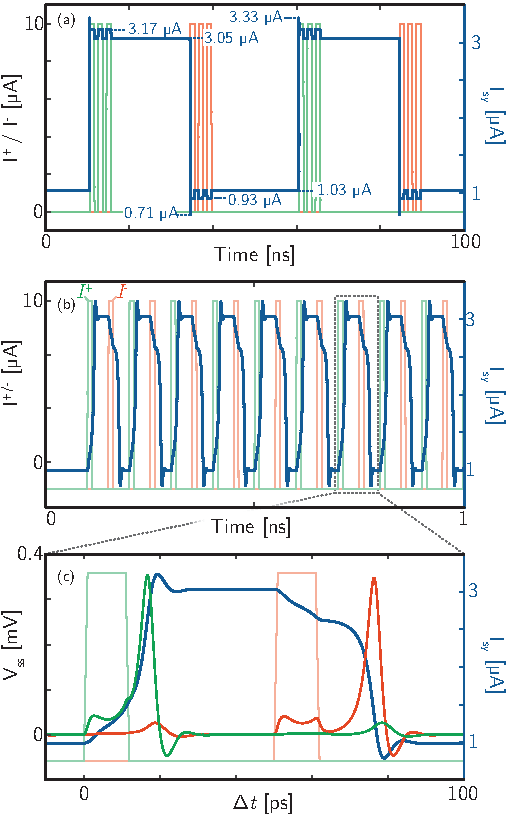
\includegraphics[width=8.6cm]{_synapticPlasticity_binary_small.pdf}}
	\caption{\label{fig:synapticPlasticity_binary}Operation of binary synapse. (a) Synaptic bias, $I_{\mathrm{sy}}$, as a function of time while potentiating and depressing drive signals are applied. The red and green traces are the drive signals across the two JJs, referenced to the left $y$ axis. The blue trace is $I_{\mathrm{sy}}$, referenced to the right $y$ axis. (b) The operation of the storage loop driven with 50 ps switching time. (c) Temporal zoom of the data in (b), with the fluxon voltage pulses generated by the switching events also shown.}
\end{figure}

Figure \ref{fig:synapticPlasticity_binary} shows WRSpice simulations of the temporal behavior of the circuit as it switches between states. In Fig.\,\ref{fig:synapticPlasticity_binary}(a), the circuit is initially in the depressed state. A pulse of 10\,\textmu A drives the circuit to the potentiated state. Repeated current pulses do not switch the state, and after the input pulses cease, the cell holds the value of $I_{\mathrm{sy}}$. Upon the application of a single 10\,\textmu A pulse into the weakening port ($I_{\mathrm{ss}}^{\mathrm{b2}}$), the circuit switches back to the depressed state, and repeated applications of this signal do not further switch the circuit.

\begin{figure}[t!]
	\centerline{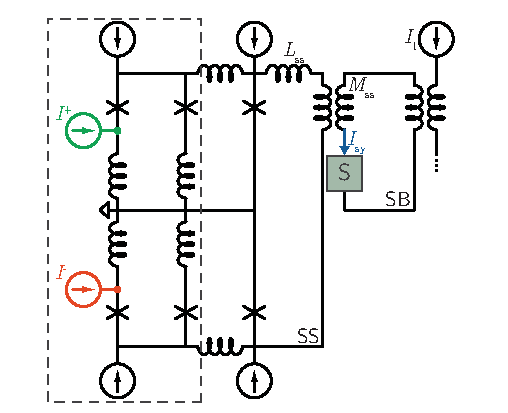
\includegraphics[width=8.6cm]{_synapticPlasticity_supervisedCircuit_small.pdf}}
	\caption{\label{fig:synapticPlasticity_supervisedCircuit} Diagram of the synaptic update circuit used for supervised learning with multiple stable synaptic values. DC-to-SFQ converters (dashed box) add fluxons to the synaptic storage loop to increase or decrease the synaptic bias current applied to the synaptic firing circuit. Values of the circuit parameters are listed in Appendix \ref{apx:circuitParameters}.}
\end{figure}
In Fig.\,\ref{fig:synapticPlasticity_binary}(b) we show the synapse switching between the depressed and potentiated states every 50\,ps. The time scale of Fig.\,\ref{fig:synapticPlasticity_binary} is extremely fast compared to biological neural circuits. The speed of these circuits offers intriguing possibilities, as discussed in Sec.\,\ref{sec:discussion_synapticPlasticity}. Figure \ref{fig:synapticPlasticity_binary}(c) shows a temporal zoom of a full cycle of the binary synapse occurring within 50\,ps. The operation considered in Fig.\,\ref{fig:synapticPlasticity_binary} is intended to show the operating range of the synapse, but in practice repeated switching in this manner is unlikely to be useful for neural operation.   

\begin{figure}[t!]
	\centerline{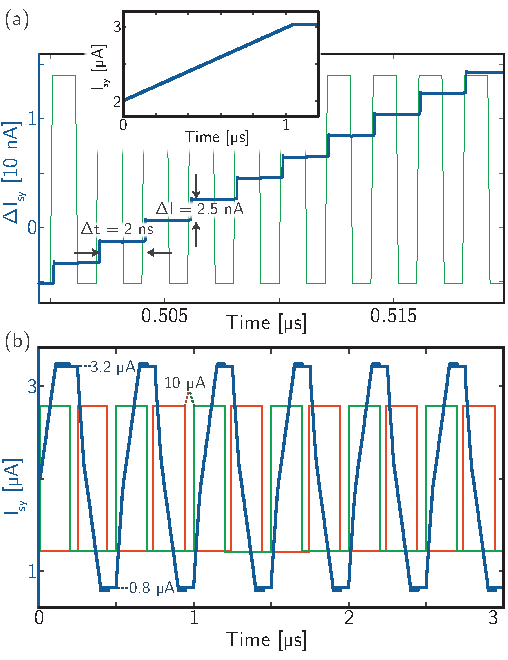
\includegraphics[width=8.6cm]{_synapticPlasticity_supervised_small.pdf}}
	\caption{\label{fig:synapticPlasticity_supervised} Operation of the synaptic update circuit for supervised learning. (a) Synaptic current bias, $I_{\mathrm{sy}}$, is shown by the blue trace, referenced to the left $y$ axis. The drive signal, $I^+$ is shown without reference to an axis. The square wave has a 10\,\textmu A amplitude and 2\,ns period. The main panel shows detail of the operation on a short time scale, and the inset shows a ramp from the middle synaptic weight until saturation at the maximum synaptic weight. In this calculation, $L_{\mathrm{ss}} = 200$\,nH, $\Delta I_{\mathrm{ss}} = 10.3$\,nA per pulse, and $\Delta I_{\mathrm{sy}} = 2.5$\,nA per pulse. (b) Schematic of the circuit used to strengthen as well as weaken synaptic weight. (c) Operation of the circuit as the synaptic weight is repeatedly ramped between minimum and maximum values.}
\end{figure}
For deep learning in neural networks, it can be advantageous to increment the synaptic weights in small steps. To achieve fine weight update, a superconducting loop capable of storing more than one flux quantum is utilized, as shown in Fig.\,\ref{fig:synapticPlasticity_supervisedCircuit}. Flux quanta can be added one by one using DC-to-SFQ converters \cite{ka1999,vatu1998}. The binary synapse has been modified to include two DC-to-SFQ converters: one for potentiating and one for depressing.  When a fluxon is produced by the potentiating DC-to-SFQ converter by the introduction of a current pulse, $I^+$, the fluxon is added to the SS loop. When a fluxon is produced by the depressing DC-to-SFQ converter by the introduction of a current pulse, $I^-$, the fluxon counter propagates in the SS loop. The inductors of the SS loop, $L_{\mathrm{ss}}$ and $M_{\mathrm{ss}}$ can be chosen over a broad range of values to determine the learning rate and range of synaptic weights achieved.

Controlled increase of synaptic bias current is again demonstrated using WRSpice. The results are shown in Fig.\,\ref{fig:synapticPlasticity_supervised}. In this calculation, a periodic square wave drives the DC-to-SFQ converter with 10\,\textmu A pulses of 1\,ns duration and 2\,ns period. Current is added to the SS loop in fluxon increments over many input cycles (Fig.\,\ref{fig:synapticPlasticity_supervised}(a)). In this case, the value of $I_{\mathrm{sy}}$ before any flux has been added to the SS loop is 2\,\textmu A, chosen to be in the middle of the operational range identified in Sec.\,\ref{sec:receiverCircuits}. For this calculation, the inductance of the SS loop is 200\,nH ($\beta_{\mathrm{L}}/2\pi = L I_c/\Phi_0 = 3.8\times 10^3$), leading to the addition of 2.5\,nA to $I_{\mathrm{sy}}$ with the addition of each fluxon to the loop. This value of inductance (and therefore $\Delta I_{\mathrm{sy}}$) can be chosen over a broad range to set the synaptic update increment and number of synaptic levels. This value was chosen to create a SS loop that can store over 1000 fluxons between the minimum and maximum values of $I_{\mathrm{sy}}$.

The inset of Fig.\,\ref{fig:synapticPlasticity_supervised}(a) shows the behavior of $I_{\mathrm{sy}}$ as a function of time as it is potentiated to saturation. A fluxon is added to the loop every two nanoseconds. After approximately 500 fluxons have been added to the loop, the value of $I_{\mathrm{sy}}$ saturates just above 3\,\textmu A. This saturation behavior is advantageous so that a learning algorithm cannot cause a synaptic weight to grow without bound. 

Figure \ref{fig:synapticPlasticity_supervised}(b) shows $I_{\mathrm{sy}}$ as a function of time as the potentiating and depressing DC-to-SFQ converters are alternately employed, analogous to the two drives of the binary synapse in Fig. \ref{fig:synapticPlasticity_binaryCircuit}. For these calculations, an SS loop with 20\,nH inductance was considered to reduce the time required to achieve saturation. Initially, $I_{\mathrm{sy}} = 2$\,\textmu A. Fluxons are added to the SS loop for 200\,ns, and $I_{\mathrm{sy}}$ reaches its maximum value of 3.2\,\textmu A. Once the SS loop reaches saturation, the value of $I_{\mathrm{sy}}$ cannot be increased. The figure further shows that after the synaptic strengthening drive is turned off, $I_{\mathrm{sy}}$ maintains its value (i.e., during the time from 200\,ns - 250\,ns). After 250\,ns, fluxons of the opposite sign begin to be added to the SS loop via the synaptic weakening drive ($I^-$), and $I_{\mathrm{sy}}$ can be driven down to the minimum value (800 nA in this case). Cycling these drives results in the periodic behavior seen in Fig. \ref{fig:synapticPlasticity_supervised}(b). During each strengthening and weakening cycle, $I_{\mathrm{sy}}$ versus time has two regions with different slopes. This is because when the current in the SS loop is outside a certain range, the DC-to-SFQ converter releases two fluxons per drive cycle. This characteristic is likely of little consequence and may be eliminated with improved circuit design, possibly by separating the DC-to-SFQ converter from the SS loop with a JTL. Numerical simulation of the circuits through periodic cycling (Figs.\,\ref{fig:synapticPlasticity_binary} and \ref{fig:synapticPlasticity_supervised}) are intended to demonstrate the range of synaptic states, the transitions between them, and saturation behavior. In practice, the synapses are unlikely to be cycled in this manner and will instead be updated as needed by the learning algorithm.

The circuits of Figs.\,\ref{fig:synapticPlasticity_binaryCircuit} and \ref{fig:synapticPlasticity_supervisedCircuit} have several strengths when used to establish the synaptic weight of a superconducting optoelectronic neuron. The nature of the flux-storage Josephson circuits enables modifying the synaptic weights as many times as necessary without material degradation. The maximum and minimum values of $I_{\mathrm{sy}}$ can be designed to achieve a broad range of operating conditions. Upon reaching the maximum and minimum values, the device saturates, eliminating the possibility of runaway values of synaptic weight. Synaptic update can be carried out in a specified number of increments based on the choice of inductance of the SS loop. The size of these increments will contribute to the learning/forgetting rate of the synapse. 

While these characteristics of the circuits are conducive to implementing a variety of training algorithms based on back propagation \cite{ni2015}, we would also like to enable systems that learn using only activity within the network. We next consider a Hebbian learning circuit, which strengthens the synaptic weight between two neurons that fire in succession. This will lead to the discussion of a circuit achieving STDP based on the timing between pre- and post-synaptic activity.
	
\subsection{\label{sec:Hebbian}Hebbian update}
\begin{figure}[t!]
	\centerline{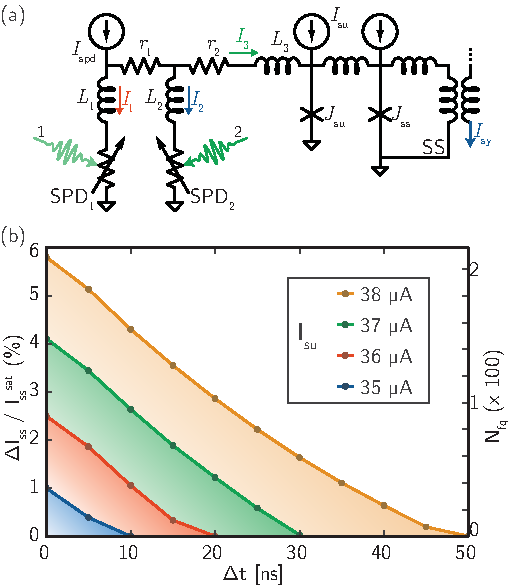
\includegraphics[width=8.6cm]{_synapticPlasticity_Hebbian_1_small.pdf}}
	\caption{\label{fig:synapticPlasticity_Hebbian_1}Hebbian update. (a) Hebbian synaptic update circuit diagram. Implements a rule based on temporally correlated single photon detection events from the two neurons associated with the synapse. Circuit parameters are given in Appendix \ref{apx:circuitParameters}. (b) Amount of current added to the synaptic storage loop, $\Delta I_{\mathrm{ss}}$, as a percentage of the saturation current of the loop, $I_{\mathrm{ss}}^{\mathrm{sat}}$, versus time delay between upstream and local synaptic update photons, $\Delta t$, for four values of $J_{\mathrm{su}}$ bias current, $I_{\mathrm{su}}$. In these calculations, $L_{\mathrm{ss}} = 1$\,\textmu H.}
\end{figure}
The Hebbian update circuit under consideration is shown in Fig. \ref{fig:synapticPlasticity_Hebbian_1}(a). The operation of this circuit is based on a similar principle to the supervised learning circuits discussed in Sec.\,\ref{sec:supervised} in that the synaptic bias current $I_{\mathrm{sy}}$ is adjusted based on the flux stored in the SS loop. The DC-to-SFQ converter of Fig.\,\ref{fig:synapticPlasticity_supervisedCircuit} can be replaced by SPDs to enable flux to be added to the SS loop based on temporally correlated photonic activity within the network. The circuit of Fig.\,\ref{fig:synapticPlasticity_Hebbian_1}(a) implements a Hebbian update rule that potentiates a synaptic connection between pre- and post-synaptic neurons when the pre-synaptic neuron contributes to the firing of the post-synaptic neuron \cite{daab2001}. 

The Hebbian rule requires a two-photon temporal-correlation circuit, like the temporal-code receiver of Sec.\,\ref{sec:receiverCircuits}, except the asymmetry of Hebbian update requires an asymmetrical initial bias to the two SPDs. Operation of the Hebbian update circuit can be described qualitatively as follows. When no photons have been detected, the bias $I_{\mathrm{spd}}$ is directed through SPD$_1$. The resistor $r_1$ ensures that SPD$_2$ is unbiased until SPD$_1$ receives a photon, and therefore photons incident on SPD$_2$ have no effect on the circuit unless they are incident during a time window following a detection event by SPD$_1$. Once a photon has been detected by SPD$_1$, $I_{\mathrm{spd}}$ is redirected to $I_2$ and $I_3$. The current returns to $I_1$ with a time constant of $\tau_1 = L_1/r_1$. If a photon is detected by SPD$_2$ during $\tau_1$, $I_{\mathrm{spd}}$ is predominantly redirected to $I_3$, which can be sufficient to switch $J_{\mathrm{su}}$, the synaptic update JJ, perhaps many times depending on the bias currents, $I_{\mathrm{spd}}$ and $I_{\mathrm{su}}$, and the difference in arrival times between the two photons, $\Delta t$. Details of circuit design are included in Appendix \ref{apx:circuitParameters}.

In Fig.\,\ref{fig:synapticPlasticity_Hebbian_1}(b) we analyze the current added to the SS loop as a function of the delay, $\Delta t$, for four values of $I_{\mathrm{su}}$ with $I_{\mathrm{spd}}$ fixed at $10~\mu$A. We plot the change in current in the SS loop ($\Delta I_{\mathrm{ss}}$) as a percentage of the SS loop saturation current ($I_{\mathrm{ss}}^{\mathrm{sat}}$) during Hebbian update events characterized by delay $\Delta t$. The amount of synaptic weight modification depends strongly on the temporal delay, dropping to zero after roughly $\tau_1$ (50\,ns in this case). We also see that the effect depends on $I_{\mathrm{su}}$, enabling the memory update rate to be dynamically adjusted during operation via a DC bias current. This dependence on $I_{\mathrm{su}}$ provides a means to implement metaplasticity. The quantity $\Delta I_{\mathrm{ss}}/I_{\mathrm{ss}}^{\mathrm{sat}}$ represents the fraction of the synapse dynamic range that is acquired in an update event. Although the current in the SS loop (and therefore $I_{\mathrm{sy}}$) can only change by an integer number of flux quanta, the use of high-kinetic-inductance flux storage loops wherein thousands of flux quanta can be stored makes this effectively an analog circuit. For the SS loop investigated in Fig.\,\ref{fig:synapticPlasticity_Hebbian_1}(a), $\beta_{\mathrm{L}}/2\pi = 1.9\times 10^4$. 

During circuit operation, we assume when the pre-synaptic neuron fires a photonic pulse, one or more photons will reach a synaptic firing circuit of the post-synaptic neuron and bring the neuron closer to its threshold, as discussed in Sec.\,\ref{sec:receiverCircuits}. We also assume additional photons have a probability of reaching SPD$_1$ of the synaptic update circuit shown in Fig.\,\ref{fig:synapticPlasticity_Hebbian_1}(a) to perform the first step in implementing the Hebbian rule. This photon is labeled ``1'' in Fig.\,\ref{fig:synapticPlasticity_Hebbian_1}(a). The probability of reaching SPD$_1$ may be controlled to modify the learning rate. Similarly, it is assumed that during a neuronal firing event, the local neuron will send photons to its downstream connections, but also to its local synaptic update circuits to activate learning by striking SPD$_2$. This photon is labeled ``2'' in Fig.\,\ref{fig:synapticPlasticity_Hebbian_1}(a). This self-feedback is also illustrated in Fig.\,\ref{fig:general_schematic}.

Hebbian learning rules may be based on average firing rates of pre- and post-synaptic neurons or on timing between individual spikes from these neurons \cite{geki2002}. Here we consider the latter. A timing-dependent learning rule often takes the form of exponential decay as a function of the difference in arrival times of pre- and post-synaptic signals. The form shown in Fig.\,\ref{fig:synapticPlasticity_Hebbian_1}(b) is slightly different due to Josephson nonlinearities. This modified temporal dependence is likely of little consequence as it maintains the principal function of timing-dependent plasticity, which is to modify the synaptic weight based on temporal correlation within a specified time window surrounding a neuronal firing event. 

While the quantity $\Delta I_{\mathrm{ss}}$ represents the change in synaptic weight due to one Hebbian update event, the area under the curves in Fig.\,\ref{fig:synapticPlasticity_Hebbian_1}(b) will be related to the learning rate when averaged over many events, because the delay between the two photons, $\Delta t$, will vary across events. The integral of the curve with $I_{\mathrm{su}} = 35$\,\textmu A is 3.6\% of the integral of the curve with $I_{\mathrm{su}} = 38$\,\textmu A. For $I_{\mathrm{su}} = 36$\,\textmu A, the value is 18\%, and for $I_{\mathrm{su}} = 37$\,\textmu A, the value is 48\%. The learning rate can be dynamically adjusted across a broad range via $I_{\mathrm{su}}$.
	
\subsection{\label{sec:stdp}Spike-timing-dependent plasticity}
Learning rules that can both strengthen and weaken the synaptic connection are required for neural computing. Spike-timing-dependent plasticity requires the Hebbian potentiating operation described in Sec.\,\ref{sec:Hebbian}, and also an anti-Hebbian depressing operation wherein a neuronal firing event at the post-synaptic neuron followed closely by a neuronal firing event at a pre-synaptic neuron depresses the synaptic weight between the two neurons. A circuit capable of producing this STDP is depicted in Fig.\,\ref{fig:synapticPlasticity_stdp}(a). The full circuit with the STDP module delivering $I_{\mathrm{sy}}$ to $J_{\mathrm{sf}}$ is shown in Fig.\,\ref{fig:transmitters_fullCircuit}. Much as strengthening and weakening were accomplished in Sec.\,\ref{sec:supervised} by adding a mirror image of the strengthening circuit to the SS loop, here we duplicate the Hebbian circuit of Sec.\,\ref{sec:Hebbian} to achieve STDP. The similarity of the SPD circuit of Fig.\,\ref{fig:synapticPlasticity_stdp}(a) and the JJ circuit of Fig.\,\ref{fig:synapticPlasticity_supervisedCircuit} is apparent. In Fig.\,\ref{fig:synapticPlasticity_stdp}(a), each SPD is assumed to be connected to a different photonic port. Two of the ports receive photons from the pre-synaptic neuron, and two of the ports receive photons from the post-synaptic neuron. In this circuit, photons coming from the pre-synaptic neuron are drawn coming from the left, and photons from the post-synaptic neuron are drawn coming from the right. 

The symmetry between the strengthening and weakening receiver circuits in the STDP circuit of Fig.\,\ref{fig:synapticPlasticity_stdp}(a) is broken based on whether the SPD that is biased in the steady state receives photons from the pre-synaptic or post-synaptic neuron. In the synaptic-weakening receiver circuit, a post-synaptic photon detected by SPD$_3$ followed by a photon from a pre-synaptic neuron detected by SPD$_4$ introduces counter-circulating flux to the SS loop. The time constants and biases of the strengthening and weakening receivers can be adjusted independently.   

To demonstrate the feasibility of implementing STDP, Fig.\,\ref{fig:synapticPlasticity_stdp}(b) shows a plot of the change in current in the SS loop versus the relative arrival time of photons at the pre- and post-synaptic detectors as calculated with WRSpice, again modeling photon detection events as transient resistance pulses. The time delay, $\Delta t$, is defined as the time of arrival of the post-synaptic photon minus the time of arrival of the pre-synaptic photon. The upper right quadrant is essentially the same as the Hebbian behavior discussed in Sec.\,\ref{sec:Hebbian}. When $\Delta t$ becomes negative, the upper portion of the circuit makes no modification to the current in the SS loop. The lower portion of the circuit is nearly identical to the upper portion, except that the pre- and post-synaptic photons are routed to the opposite SPDs, and current added to the SS loop by the lower portion circulates in the opposite direction as when added by the upper portion of the circuit. Thus, the lower portion of the circuit only adds flux to the SS loop when the post-synaptic photon arrives before the pre-synaptic neuron, and in this anti-Hebbian event, the synaptic weight is weakened. In both the Hebbian and anti-Hebbian cases, this model indicates the synaptic update abruptly drops to zero when the photon arrival times are in the reverse order. In practice, this effect would be smeared out by the timing jitter of the light sources and detectors, and the synaptic update represented in Fig.\,\ref{fig:synapticPlasticity_stdp}(b) would be convoluted with the source and detector jitter when averaged over many firing events.

To gain intuition regarding the dynamical operation of the STDP circuit, Figs.\,\ref{fig:synapticPlasticity_stdp}(c) and (d) illustrate the circuit in operation, as simulated with WRSpice. Two synaptic strengthening events and two synaptic weakening events occur. The currents associated with synaptic strengthening and weakening, $I^+$ and $I^-$, are shown in Fig.\,\ref{fig:synapticPlasticity_stdp}(c) with colors related to the currents labeled in Fig.\,\ref{fig:synapticPlasticity_stdp}(a). $I_{\mathrm{sy}}$ delivered to $J_{\mathrm{sf}}$ is shown in Fig.\,\ref{fig:synapticPlasticity_stdp}(d). 
\begin{figure}[t!]
	\centerline{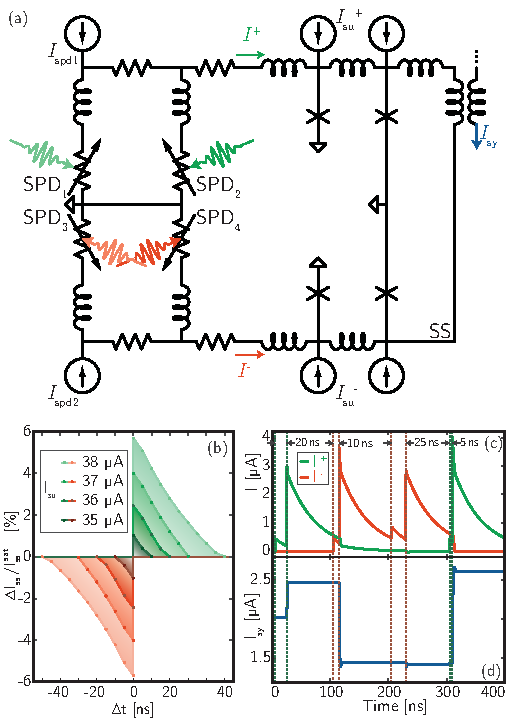
\includegraphics[width=8.6cm]{_synapticPlasticity_stdp_small.pdf}}
	\caption{\label{fig:synapticPlasticity_stdp}Implementation of spike-timing-dependent plasticity. (a) Circuit under consideration. (b) Change is current stored in SS loop as a percentage of the total storage capacity of the loop versus the relative arrival time of the two photons involved, $\Delta t$.  (c) The currents $I^+$ and $I^-$ during synaptic update events. (d) The synaptic bias current, $I_{\mathrm{sy}}$, delivered to the synaptic firing circuit as a function of time as the synaptic update events of (c) strengthen and weaken the synaptic connection. The vertical dashed lines indicate photon arrival times.}
\end{figure}
A synaptic strengthening event occurs with $\Delta t = 20$\,ns, followed by a weakening event with $\Delta t = 10$\,ns and another with $\Delta t = 25$\,ns. A final strengthening event occurs with $\Delta t = 5$\,ns. The synaptic bias current, $I_{\mathrm{sy}}$, is observed to respond as expected based on the Hebbian analysis in Sec.\,\ref{sec:Hebbian}. In this calculation, $L_{\mathrm{ss}} = 20$ nH, and we mention again that the amount of current added to $I_{\mathrm{ss}}$ and therefore $I_{\mathrm{sy}}$ during a synaptic update event can be linearly scaled with $L_{\mathrm{ss}}$ in hardware and with $I_{\mathrm{su}}$ dynamically. The memory update rate of the STDP synapse can be controlled by adjusting the frequency of photon absorption events.

While crucial to learning and the interplay between the structure and function of neural systems, STDP is only one of many synaptic plasticity mechanisms. Despite their significance, we do not discuss short-term plasticity, homeostatic plasticity, or metaplasticity here. Further investigation of these circuits will be the subject of future work.
	
\subsection{\label{sec:discussion_synapticPlasticity}Discussion Regarding Synaptic Plasticity}
This section has explored synaptic update circuits capable of delivering a variable synaptic bias current to the synaptic firing circuits presented in Sec.\,\ref{sec:receiverCircuits}. Manipulation of the synaptic weight through external input of square wave pulses and via photon detection events has been simulated. 

For STDP, the synaptic update circuits described here provide ports for four photons: one strengthening photon from both the pre\textendash synaptic and post\textendash synaptic neuron, and one weakening photon from both the pre\textendash synaptic and post\textendash synaptic neuron. For a single synaptic strengthening or weakening event, two of these photons must be present. When optically implementing a synaptic update rule based on timing correlation, it is difficult to achieve a circuit requiring fewer than two photons.

Other forms of photonic synapses have recently been developed and offer utility in multiple neural contexts \cite{prsh2017,tana20142,tafe2017,shha2016,chri2017,humi2018}. One can leverage phase shifts in microrings \cite{tana20142,tafe2017} or Mach-Zehnder interferometers (MZIs) \cite{shha2016} to adjust synaptic weight. Thermal tuning is often employed to implement the phase shifts. Thermal tuning requires more power than is suitable for this hardware platform. Phase shifters may also be large if MZIs are used, and phase shifters may require exotic materials that limit scaling if electro-optic effects are leveraged. If different synapses are addressed with different frequencies of light, the out-degree of a node in the network is limited by the multiplexed channel spacing. Approaches using MZIs for weighting and routing have the disadvantage that STDP cannot be implemented, because modifying a single phase shifter in the network affects many synaptic weights. One approach to synaptic weighting in the photonic domain utilizes a variable optical attenuator at each synaptic connection. Phase-change materials have been employed as such variable attenuators \cite{chri2017}, and the absorption of phase-change materials can be affected with pulses of light, thus introducing a Hebbian-type synaptic weight update process. While such an approach may be useful for certain types of neural circuits, update of these synapses requires too many photons to be useful for the neural computing scheme developed here (billions of photons per update operation for phase change versus single photons for superconducting optoelectronics). It is also not clear how anti-Hebbian synaptic update can be introduced to enable full spike-timing-dependent plasticity. It remains to be seen if other synaptic operations such as short-term plasticity, homeostatic plasticity, and metaplasticity can be achieved with phase-change materials. Synaptic weights that attenuate a signal in the optical domain require more light from neuronal firing events, and many photons are simply absorbed at weak synapses. By contrast, using photons for communication but weighting in the superconducting domain uses fluxons to change the synaptic weight, and they can be generated with orders of magnitude less energy than photons. While all of these approaches to synaptic weighting may be useful in different contexts, we have developed the synapses presented in this work based on simultaneous considerations of power, complexity, scalability, speed, and size in the context of the superconducting optoelectronic hardware platform.

An important weakness of the synapses presented here is they lose all memory when superconductivity is broken. The neuromorphic system must remain below $T_{\mathrm{c}}$ to preserve what has been learned. This class of Frosty the Snowman memory may be augmented by devices that can be heated, such as magnetic Josephson junctions \cite{ru2016,scdo2017,scdo2018}. It would be appealing if the state of memory in the plastic synapses described here could be transferred to long-term magnetic memory, perhaps during a sleep phase.

Another potential challenge for this type of loop neuron memory is flux trapping. The SI loops discussed in Sec.\,\ref{sec:receiverCircuits} are likely to include resistors to give a leak rate. Trapped flux in those loops will be less problematic. The SS loops that set the synaptic weights are intended to store flux for a long time to maintain memory, so they will not include resistors. Trapped flux will produce variations in the initial synaptic weights across an ensemble. For binary synapses, this will result in some synapses being initialized with strong synaptic weight, and some with weak. For SS loops with high inductance, stray flux will induce a small current, so the perturbation may be small relative to the dynamic range of the synapse. For large ensembles of synapses, the statistical variation may be tolerable or even advantageous. If flux proves problematic, techniques used to shield superconducting qubits can be employed \cite{coch2011}.

In Sec.\,\ref{sec:introduction} we argue that a dynamical system capable of differentiated processing and information integration across spatial and temporal scales underlies cognition. In Sec.\,\ref{sec:receiverCircuits} we introduced the relaxation oscillators and dendritic processing loops capable of implementing the temporal synchronization operations necessary for integrating information in time. Network synchronization and synaptic plasticity are mutually constructive phenomena, in that synaptic strengthening through spike timing is more likely to occur when the firing of two neurons is correlated, and the strengthened synapses, in turn, make the correlated neurons more likely to synchronize. Networks with small-world structure \cite{wast1998,sp2010} and dynamics characterized by self-organized criticality are crucial to achieving information integration. Hebbian learning rules and STDP have been shown to convert random networks into small-world networks and to give rise to self-organized criticality \cite{siqu2007,rusp2011}. Creation of hardware capable of supporting complex networks and synaptic learning mechanisms will provide a powerful tool for the investigation of the relation between critical network dynamics and cognitive function. We have shown some of the complex synaptic behaviors necessary for rapid adaptation, long-term memory retention, and synaptic update based on network activity. Networks of neurons connected by these synapses will be capable of integrating information learned at many times in many contexts in a single dynamical state.

%---------------------------------------------
%transmitters
%---------------------------------------------	
\section{\label{sec:transmitterCircuits}Transmitter Circuits}
%\input{transmitters_introduction}	
Synaptic receivers must partner with a light source to generate a neuronal firing event when the integrated current reaches a threshold. In Sec.\,\ref{sec:receiverCircuits} we discuss how a JJ could be used as a thresholding element. In this section, we show that the flux quantum generated by a thresholding JJ can trigger an amplification sequence resulting in an optical pulse containing one to 100,000 photons. These superconductor/semiconductor hybrid circuits achieve electrical-to-optical transduction and facilitate communication with high fanout and light-speed delays in complex networks of superconducting optoelectronic neurons. We refer to these amplifier circuits as the transmitter of the neuron.

\begin{figure}[t!]
	\centerline{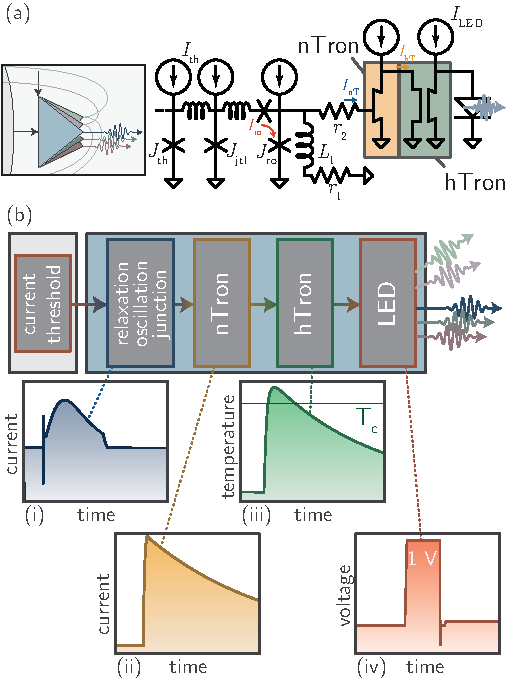
\includegraphics[width=8.6cm]{_transmitters_schematic_small.pdf}}
	\caption{\label{fig:transmitters_schematic}(a) Circuit diagram of the amplifier chain under consideration showing the thresholding JJ, relaxation-oscillator JJ, nTron, hTron, and LED. The small box shows the corresponding portion of the schematic Fig.\,\ref{fig:general_schematic}. (b) Sequence of events during neuronal firing event. (i) Current threshold is reached in the neuronal thresholding loop, causing the relaxation oscillation junction to produce transient current to the nTron gate. (ii) Current from the relaxation oscillator junction drives the gate of the nTron normal, causing the nTron channel current to be diverted to the gate of the hTron. (iii) The current from the nTron through the gate of the hTron drives the channel of the hTron normal, resulting in a voltage pulse across the hTron. (iv) The LED is in parallel with the hTron, so the voltage across the hTron results in a voltage across the LED. This voltage is sufficient to forward-bias the $p-n$ junction to produce light.}
\end{figure}
	
A central technical challenge in designing superconducting optoelectronic hardware is to produce optical signals at telecommunication wavelengths with superconducting electronic circuits. The superconducting energy gap \cite{ti1996} is in the millivolt range, making it difficult for superconducting circuits to produce the one volt needed to appreciably alter the carrier concentrations in semiconductor electronic and optoelectronic devices. This voltage mismatch makes it difficult for superconducting electronic circuits to interface with CMOS logic \cite{ka1999} and memory \cite{vafe2002}. 

A common approach to increase voltage in superconducting circuits is to place JJs in series \cite{suin1988}. The achievable voltage scales as the superconducting energy gap multiplied by the number of junctions. Order one thousand junctions must be utilized to drive the light sources we intend to employ \cite{shbu2017,buch2017,bu2018}. While superconducting circuits operate at low voltage, they can sustain large current. Supercurrent can be converted to voltage with a resistor. A microamp across a megaohm produces a volt. A small meandering wire of a superconducting thin film can easily produce a megaohm resistance in the normal-metal state. Thus, we can convert a current-biased superconducting wire into a voltage source by switching the wire between the superconducting and normal states.

Such a voltage source is not commonly used in superconducting electronics because it tends to be slow and consume more energy per operation than a JJ. The advantages of superconducting electronics for digital computing are largely speed and efficiency, while the advantages of superconducting optoelectronic networks are largely \textit{communication} and efficiency. While superconducting electronics aspire to operate above 100\,GHz, superconducting optoelectronic networks comprising neurons firing up to 20\,MHz would be a radical increase relative to the maximum frequency of 600\,Hz in biological neural systems \cite{stsa2000,budr2004,bu2006}. The goal of neural rather than digital computing liberates us to use superconducting devices slower than JJs for events that only occur once per neuronal firing. The speed and efficiency of JJs are still leveraged by loop neurons to distinguish synaptic efficacy during each synaptic firing event. Thus, we can use a switching element leveraging the superconductor-to-normal phase transition in a neural context, provided it operates every neuronal firing event and not every synaptic firing event. 

An effective means of breaking the superconducting phase is to heat the wire locally. Thermal devices are generally slow and power hungry, but the small volume, small temperature change, and small heat capacity at low temperature \cite{lasa1988,du2015} enable switching times on the order of a nanosecond with femtojoules of energy. While such an amplifier is not suitable for the high speed and low power of flux-quantum logic \cite{hehe2011,mu2011,li2012,taoz2013}, a single firing of the switch can produce thousands of photons, making it very useful and efficient in this neural context where each synapse can be activated by a single photon.

This high-impedance, phase-change switch is called an hTron \cite{zhto2018}. The heating operation required to switch the hTron from the superconducting to metal state can be achieved through dissipation in a Joule heater. Fairly large current is required to provide sufficient power. While the hTron is equipped to deliver voltage to drive the semiconductor light source, the thresholding JJ will provide only fluxons when the neuron's threshold is reached. These fluxons are insufficient to thermally switch the state of the hTron. An intermediate current amplifier is therefore required to convert fluxons from the thresholding JJ into current across the Joule heating element of the hTron. For this step of the amplification process, an nTron \cite{mcbe2014} will suffice. The nTron is a three-terminal thin-film superconducting current amplifier. A small current in the constricted gate can exceed the local critical current and drive the path from source to drain normal. An impedance on the order of a kilohm can be produced quickly, and the current from the source to drain will be diverted to a load. In the present case, that load is the $\approx$\,10\,$\Omega$ resistive element of the hTron. 

A summary of the circuit operation is shown in Fig. \ref{fig:transmitters_schematic}. The schematic and circuit diagram are shown in Fig.\,\ref{fig:transmitters_schematic}(a), and the sequence of events in the operation of the transmitter is shown in Fig.\,\ref{fig:transmitters_schematic}(b). The NT loop described in Sec.\,\ref{sec:receiverCircuits} reaches threshold due to integrated current from synaptic firing events, and the thresholding JJ produces one or more fluxons. These fluxons enter the gate of the nTron, exceeding the gate critical current. The nTron source/drain current is then diverted to the hTron gate. Joule heating in the hTron gate produces a temperature shift of several kelvins, switching the hTron to the high-impedance state. The hTron source-drain current suddenly experiences 1\,M$\Omega$, and the current rapidly switches to first charge the LED capacitor and then, once sufficient voltage is achieved across the capacitor, current is driven through the diode. This current generates photons through electron-hole recombination. These photons are the optical source for neural communication.

This amplifier circuit is relatively complex and uses the most power of any part of the neural circuit. A more elegant solution may be possible. Any solution must meet several operating criteria: 1) the transmitter must threshold on a low-current signal from the NT loop; 2) the amplifier chain must convert this signal to the voltage necessary to produce light from a semiconductor diode; 3) the operation should happen at least as fast as the recovery of the single-photon detectors in the loop neuron synapses (a few tens of nanoseconds); 4) a number of photons appropriate to communicate with the neuron's synaptic connections must be produced; 5) the number of photons created must be dynamically variable with a bias current; 6) the energy of a firing event must be low enough that an ensemble of neurons in realistic network operation have power density low enough for heat to be removed by liquid helium; 7) total power consumption must be low enough to enable scaling to neural systems with billions of interacting nodes. The transmitter circuits presented here satisfy these criteria. We begin with the design of the hTron driving the LED and work backward through the circuit of Fig.\,\ref{fig:transmitters_schematic}(a).
	
\subsection{\label{sec:LED}Driving the light-emitting diode}
We must ensure the voltage required to drive the LED can be sustained for a duration commensurate with the number of photons required. This duration will depend on the drive current, the capacitance of the LED, the efficiency of the LED, and the number of synaptic connections served by the neuron. Once the drive requirements of the LED are understood, we can proceed to design an hTron that can meet these drive requirements.

The LED circuit under consideration is shown in Fig.\,\ref{fig:transmitters_LED_circuit}. The LED is modeled as a variable resistor in parallel with a capacitor. The variable resistor is modeled with the DC $I-V$ characteristic of a $p-n$ junction, as described in Appendix \ref{apx:circuitParameters}. The hTron is modeled as a variable resistor in series with an inductor. This variable resistor is treated as a step function with zero resistance abruptly switching to 800\,k$\Omega$. This model is intended to capture the behavior of the hTron driving the LED as the superconducting channel of the hTron is driven above its transition temperature. A thermal model of the hTron is presented in Sec.\,\ref{sec:hTron}.
\begin{figure}[t!]
	\centerline{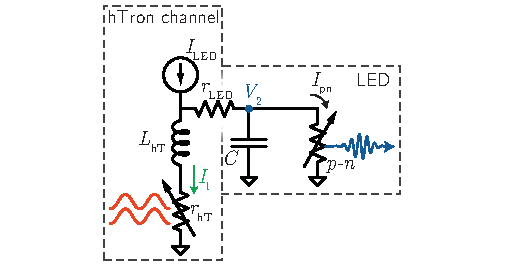
\includegraphics[width=8.6cm]{_transmitters_LED_circuit_small.pdf}}
	\caption{\label{fig:transmitters_LED_circuit}Circuit diagram of the LED driven by the hTron. For this analysis, the hTron channel is modeled as a variable resistor ($r_{\mathrm{hT}}$) in series with an inductor ($L_{\mathrm{hT}}$). The LED is modeled as a capacitor, $C$, in parallel with a variable resistor (labeled $p-n$). The hTron variable resistor switches under the influence of heat produced by Joule heating in the gate resistive element, discussed in Sec.\,\ref{sec:hTron} (see also Appendix \ref{apx:circuitParameters}). The LED variable resistor models the DC current-voltage characteristic of the $p-n$ junction (see Appendix \ref{apx:circuitParameters}). The hTron channel is biased with $I_{\mathrm{LED}}$. When the channel is driven normal, $r_{\mathrm{hT}}$ switches from 0\,$\Omega$ to $800$\,k$\Omega$. The current charges up the capacitor until the voltage is $\approx$\,1\,V, at which point current begins to flow through the $p-n$ junction, producing light.}
\end{figure}

The equations of motion for the circuit of Fig.\,\ref{fig:transmitters_LED_circuit} are given in Appendix \ref{apx:circuitParameters}. Solving these equations, we obtain the circuit currents and voltages as a function of time. From these quantities, we can determine the energy dissipated during a firing event as well as the number of photons produced. The number of photons produced is calculated as 
\begin{equation}
\label{eq:Nph}
N_{\mathrm{ph}} = \frac{\eta_{\mathrm{qe}}}{e}\int I_{pn} dt, 
\end{equation}
where $\eta_{\mathrm{qe}}$ is the quantum efficiency of the diode, and $e$ is the electron charge. The efficiency of the circuit of Fig.\,\ref{fig:transmitters_LED_circuit} is calculated as $
\eta_{RC} = h \nu N_{\mathrm{ph}} / E_{RC}$, where $h$ is Planck's constant, $\nu$ is the frequency of a photon (taken to be $c/1.22$\,\textmu m \cite{buch2017}), and $E_{RC}$ is the total energy dissipated by the $RC$ circuit of Fig.\,\ref{fig:transmitters_LED_circuit} during a firing event as calculated with the model given in Appendix \ref{apx:circuitParameters}. 

At least two other factors will contribute to the efficiency of the circuit in Fig.\,\ref{fig:transmitters_LED_circuit}. First, carriers injected into the $p-n$ junction may recombine non-radiatively. This loss mechanism is captured in the internal quantum efficiency, $\eta_{\mathrm{qe}}$. Second, light generated by electron-hole recombination events may not couple to the guided mode of the axonal waveguide, and will therefore not couple to the synaptic terminals. This loss mechanism is captured in the waveguide coupling efficiency, $\eta_{\mathrm{wg}}$. The total LED efficiency is given by $\eta_{\mathrm{LED}} = \eta_{RC}\,\eta_{\mathrm{qe}}\,\eta_{\mathrm{wg}}$.

Circuit performance is shown in Fig.\,\ref{fig:transmitters_LED_data}. Voltage transients across the $p-n$ junction are shown in Fig. \ref{fig:transmitters_LED_data}(a), where two values of capacitance and two values of quantum efficiency are considered. For each of the four traces, the hTron pulse duration was chosen to produce 10,000 photons. We assume that 10 photons are generated per out-directed synaptic connection to compensate for loss, reduce noise, and implement learning functions. Thus, these voltage pulses are appropriate to neurons with out-degree of 1000. If the LED capacitance can be made as low as 10\,fF, and $\eta_{\mathrm{qe}}$ can be made as high as 0.1, the hTron gate must only be normal for 2.9\,ns. Under these operating conditions, 25\,fJ of energy is dissipated, of which 64\% is dissipated as current through the $p-n$ junction ($\eta_{RC}=0.64$). If the LED performance is worse, with $C = 100$\,fF and $\eta_{\mathrm{qe}} = 0.01$, the drive must be applied for 29\,ns. This operation dissipates 251\,fJ of energy, also with 64\% through the junction.
\begin{figure}%[t!]
	\centerline{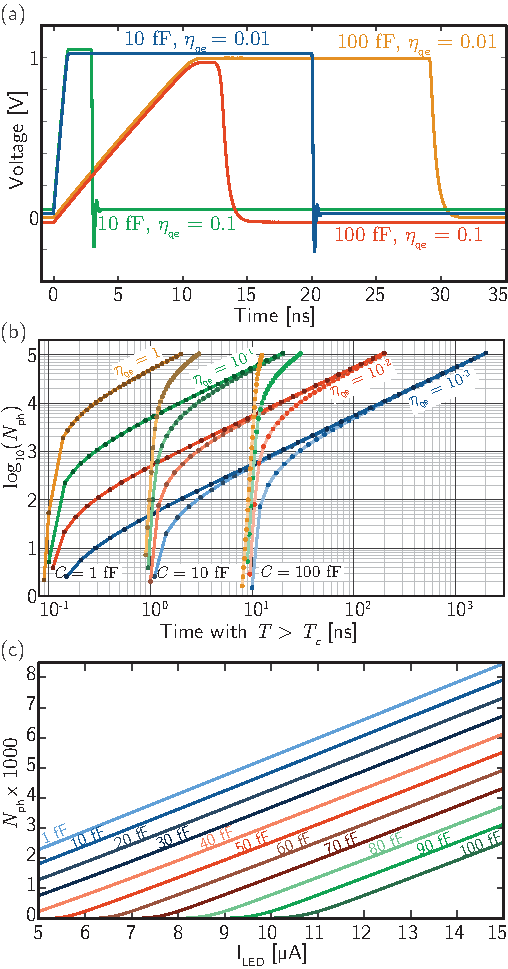
\includegraphics[width=8.6cm]{_transmitters_LED_data_small.pdf}}
	\caption{\label{fig:transmitters_LED_data}Time-domain analysis of the circuit of Fig. \ref{fig:transmitters_LED_circuit}. (a) Voltage transients for two values of LED capacitance (10 fF and 100 fF) and two values of LED quantum efficiency (0.1 and 0.01). For each of the four calculations, the hTron channel resistance was modeled as a square pulse of duration necessary to achieve 10,000 photons. Traces slightly shifted in $y$ for disambiguation. (b) The number of photons produced by the LED as a function of the time the hTron channel was held above $T_{\mathrm{c}}$. For short pulse durations, the traces group based on the capacitance, while for long pulse durations the traces group based on LED quantum efficiency. (c) The number of photons produced by the LED as a function of the current bias for several values of the LED capacitance. Here the hTron channel was held above $T_{\mathrm{c}}$ for 10\,ns. The slope of the traces ranges from 617 photons per \textmu A with $C = 1$\,fF to 584 photons per \textmu A with $C = 100$\,fF. }
\end{figure}

General trends for the number of photons produced by the circuit as a function of the time the hTron gate is above $T_{\mathrm{c}}$ are shown in Fig.\,\ref{fig:transmitters_LED_data}(b) for several values of capacitance and quantum efficiency. In these calculations, the bias current ($I_{\mathrm{LED}}$) is fixed at 10\,\textmu A. The capacitance determines the minimum hTron pulse duration necessary to achieve the voltage necessary for photon production, and the quantum efficiency determines the slope ($y$-intercept of this log-log plot) for longer hTron pulses.

As implied by the gain drive current depicted in Fig.\,\ref{fig:general_schematic}, we would like a means to dynamically control the number of photons produced in a firing event. We can achieve this by varying the bias current diverted to the LED when the channel of the hTron becomes resistive, $I_{\mathrm{LED}}$. In Fig.\,\ref{fig:transmitters_LED_data}(c) we show $N_{\mathrm{ph}}$ as a function of $I_{\mathrm{LED}}$ for various values of the LED capacitance in a case where the hTron channel is driven normal for 10\,ns and the LED quantum efficiency is assumed to be 0.01 \cite{doro2017}. This current bias provides a means to change the strength of neuronal activity. With fewer photons produced, the probability of reaching distant connections diminishes. With more photons produced, the neuron makes a stronger contribution to network activity. The synapses considered in this work do not decode the amplitude of the photonic signal, so the objective of changing the number of photons produced in a neuronal firing event is not to encode information, but rather to adjust how many synaptic connections are reached. The routing architecture can be designed so that with a given value of $I_{\mathrm{LED}}$ some synapses receive 10 photons on average from a synaptic firing event, while others receive only one. By decreasing $I_{\mathrm{LED}}$, the strongest synapses will still receive more than one photon, while the weakest will receive less than one and are effectively eliminated. Thus, $I_{\mathrm{LED}}$ provides an additional means to adapt the structural network into multiple functional networks at different times. This current bias may be modified by a supervisory user or by internal activity within the network.

The efficiency of the light-production circuit is considered with the rest of the transmitter circuit in Sec.\,\ref{sec:efficiency}. Based on the calculations of this section, we know the hTron drive requirements for light production across a range of capacitance and quantum efficiency values. If a neuron needs to produce 10,000 photons to communicate to 1000 synaptic connections, an hTron biased with a channel current of 10\,\textmu A must produce a resistance of 800\,k$\Omega$ for 1\,ns - 100\,ns, depending on the achievable LED performance. We now proceed to consider the operation of an hTron when driven by the current from an nTron.  
	
\subsection{\label{sec:hTron}The hTron voltage amplifier driven by the nTron current amplifier}
To produce the voltage across the LED required to generate light, a resistance of 800\,k$\Omega$ must be established rapidly and sustained for 1\,ns - 100\,ns. One way to achieve this is to switch a length of superconducting wire to the normal metal state. This can be straightforwardly accomplished by raising the temperature of a superconducting wire above $T_{\mathrm{c}}$. An hTron is a device that switches a channel resistance from zero ohms to a large value when current is driven through the gate \cite{zhto2018}. The current through the gate dissipates power in a resistive element through Joule heating, and this power locally raises the channel above $T_{\mathrm{c}}$. We show a schematic in Fig.\,\ref{fig:transmitters_hTron_circuit}(a), wherein a resistive layer is separated from a nanowire meander by a thin insulator. 
\begin{figure}[t!]
	\centerline{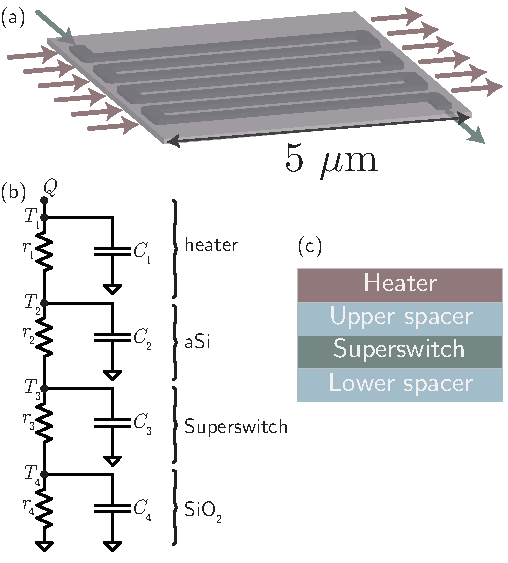
\includegraphics[width=8.6cm]{_transmitters_hTron_circuit_small.pdf}}
	\caption{\label{fig:transmitters_hTron_circuit}The hTron voltage amplifier. (a) Schematic of the thin-film configuration with a normal-metal resistive layer (gate) over the superconducting nanowire meander (channel). (b) Thermal circuit model used to calculate the dynamics of the device. (c) Cross-sectional view of layers involved in calculation.}
\end{figure}

While thermal devices can be too slow and consume too much power for some applications, there are several reasons why the hTron is suitable for the present purpose. First, the device has a compact footprint of 5\,\textmu m\,$\times 5$\,\textmu m, so a very small mass must be heated. Second, the specific heat of all materials involved falls as $T^3$, so at the desired operating temperature of 4.2\,K, the specific heat is orders of magnitude smaller than at room temperature. Third, the required temperature swing is small ($\approx 2$\,K). These factors taken together make the hTron a suitable device to achive the voltage necessary to produce light from a semiconductor diode with the power and speed required for the neural application under consideration.

To quantify the performance of the hTron when driving the LED of Sec.\,\ref{sec:LED}, we consider the transient dynamics of the thermal circuit shown in Fig.\,\ref{fig:transmitters_hTron_circuit}(b). A heat source $Q$ is delivered to the stack of materials shown in Fig.\,\ref{fig:transmitters_hTron_circuit}(c). The equations of motion and material parameters used in these calculations are given in Appendix \ref{apx:circuitParameters}. Figure\,\ref{fig:transmitters_hTron_data_1}(a) shows temperature transients of the superconducting layer when power is delivered to the hTron gate long enough to drive the hTron channel normal for 1\,ns and for 10\,ns. In this plot, the hTron gate is driven with square current pulses to illustrate the temporal dynamics of the thermal components. In this model, the hTron can switch to the resistive state in roughly 1\,ns. While this time scale is not suitable for many operations in superconducting digital electronics, it is more that fast enough for a neuronal firing event in the system under consideration.  
\begin{figure}[t!]
	\centerline{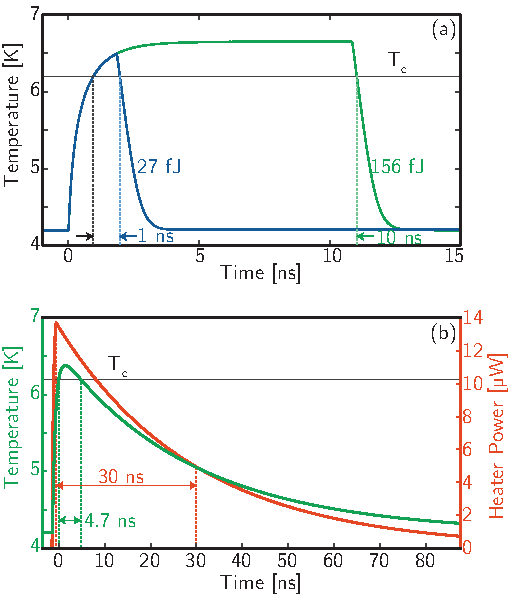
\includegraphics[width=8.6cm]{_transmitters_hTron_data_1_small.pdf}}
	\caption{\label{fig:transmitters_hTron_data_1}Time-domain analysis of the hTron. (a) A square current pulse is driven through the gate of the hTron. Two traces are shown for cases when the channel was driven normal long enough to keep the the temperature above $T_{\mathrm{c}}$ for 1\,ns and 10\,ns. (b) An exponential current pulse is driven through the gate of the hTron, as would be the case when the nTron is used to drive the hTron. In the case shown, the $L/r$ time constant of the nTron is 30\,ns, and the channel of the hTron is held above $T_{\mathrm{c}}$ for 4.7\,ns.}
\end{figure}

While a square pulse is most efficient for driving the hTron, exponentially rising and decaying pulses will be generated by the nTron \cite{mcbe2014}. The nTron is a three-terminal, thin-film device. In the off state, a supercurrent flows from the source to drain, and the gate is in the superconducting state. The gate comprises a small constriction, and when the current delivered to the gate exceeds the critical current, it is driven locally to the normal state. Joule heating spreads the normal domain, and quickly causes the channel between the source and drain to be driven normal across the entire wire width. This normal domain provides a few squares of resistance (roughly 1\,k$\Omega$), at which point the source-drain current is diverted to a load. In the present case, the load is the gate of the hTron (10\,$\Omega$ in this study, the resistance of the upper layer in Fig.\,\ref{fig:transmitters_hTron_circuit}(a) and (c)). When the gate current to the nTron ceases and the channel returns to the superconducting state, the channel current returns with the $L/r$ time constant of the system. Thus, the current pulse from the nTron to the hTron will have an exponential time dependence. 

In Fig.\,\ref{fig:transmitters_hTron_data_1}(b) we show the temporal response of the hTron channel temperature when the gate is driven by an exponential current pulse of 1.2\,mA amplitude from an nTron. In this case, the rise time of the pulse is 300\,ps, and the fall time is 30\,ns. These time constants are controlled by the $L/r$ time constants of the circuit. The fall time is set by $L_{\mathrm{nT}}/r_{\mathrm{nT}}$, where $L_{\mathrm{nT}}$ is the inductance of the nTron channel, and $r_{\mathrm{nT}}$ is the load of the nTron, which in this case is the gate resistance of the hTron. To achieve the power necessary to switch the hTron, 1.2\,mA from the nTron is required across the 10\,$\Omega$ of the hTron gate.

Driving the hTron with the exponential pulses of the nTron is far less efficient than driving with square pulses, because power continues to be dissipated in the exponential tail of the current pulse long after the temperature of the hTron channel drops back below $T_{\mathrm{c}}$. In the case considered in Fig.\,\ref{fig:transmitters_hTron_data_1}(b), the $L_{\mathrm{nT}}/r_{\mathrm{nT}}$ time constant is 30\,ns, and the hTron channel is held above $T_{\mathrm{c}}$ for 4.7\,ns. A square pulse of 6\,ns would achieve the same duration of the hTron in the resistive state. Figure \ref{fig:transmitters_hTron_data_2}(a) illustrates this inefficiency. The required $L_{\mathrm{nT}}/r_{\mathrm{nT}}$ time constant is plotted as a function of the time the hTron channel must be held above $T_{\mathrm{c}}$, referred to as $t_{\mathrm{hot}}$. The time $t_{\mathrm{hot}}$ depends on the LED capacitance, efficiency, and the number of photons produced during the pulse, which is determined by the number of synapses formed by the neuron. The $L_{\mathrm{nT}}/r_{\mathrm{nT}}$ time constant must be nearly ten times $t_{\mathrm{hot}}$. Improved drive circuit designs are likely possible, but we proceed with the single-nTron example to illustrate that even with first-generation circuit designs, sufficient efficiency can be achieved. 

We wish to connect the number of photons produced in a neuronal firing event to the $\tau_{\mathrm{nT}}$ time constant that must be implemented in hardware. In Sec.\,\ref{sec:networks} we study networks with neurons making 20-1000 synaptic connections. We would like neuronal firing events to produce ten times as many photons as the neuron's out-degree to compensate for loss, reduce noise, and perform memory update operations. We are therefore interested primarily in neuronal firing events producing 200-10,000 photons, and large hub neurons may need to produce 100,000 photons or more. Such photon numbers will require the hTron channel to be driven normal for some duration, which necessitates current drive from the nTron to the hTron gate for some proportional duration (Fig.\,\ref{fig:transmitters_hTron_data_2}(a)). We therefore must calculate the number of photons produced by the LED as a function of the $\tau_{\mathrm{nT}} = L_{\mathrm{nT}}/r_{\mathrm{nT}}$ time constant, taking the LED capacitance and efficiency into account. The results of these calculations are shown in Fig.\,\ref{fig:transmitters_hTron_data_2}(b). To produce 200 photons from an LED with 10\,fF capacitance and 1\% efficiency, $\tau_{\mathrm{nT}}$ must be 8\,ns, and to produce 10,000 photons $\tau_{\mathrm{nT}}$ must be 100 ns. An nTron channel inductor achieving this time constant and carrying the requisite 1.2\,mA necessary to drive the hTron gate can be achieved in an area commensurate with the area required for the synaptic wiring and routing waveguides comprising the dendritic and axonal arbors of the loop neurons. 

\begin{figure}[t!]
	\centerline{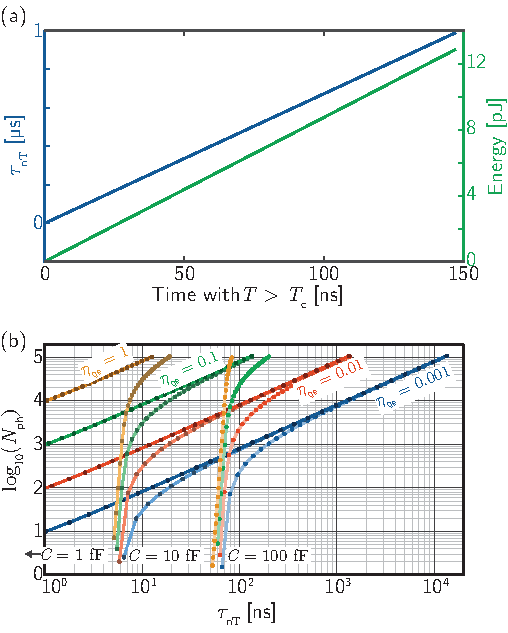
\includegraphics[width=8.6cm]{_transmitters_hTron_data_2_small.pdf}}
	\caption{\label{fig:transmitters_hTron_data_2}(a) nTron time constant required and energy consumed as a function of the time the hTron is held above $T_{\mathrm{c}}$. The energy efficiency is nearly an order of magnitude higher when the hTron is driven by a square pulse. (b) The number of photons produced by the LED as a function of the nTron $L/r$ time constant, $\tau_{\mathrm{nT}}$, for several values of LED efficiency and capacitance.}
\end{figure}
The next task is to show a JJ in the NT loop delivering the current to switch the gate of the nTron.
	
\subsection{\label{sec:detectingThreshold}Detecting neuronal threshold}
The circuit considered for detecting threshold in the NT loop is shown in Fig.\,\ref{fig:transmitters_schematic}(a). The parameters are given in Appendix \ref{apx:circuitParameters}. When the current in the NT loop reaches the switching current of the thresholding junction, $J_{\mathrm{th}}$, that junction will transmit a fluxon to the relaxation oscillator junction, $J_{\mathrm{ro}}$. A relaxation oscillator junction has the property that, upon switching, it temporarily enters a latched state. In the latched state, the junction is resistive, and the bias current is diverted to a load. A relaxation oscillator junction can be physically implemented by utilizing only the internal shunting of a superconductor-insulator-superconductor junction, resulting in a hysteretic current-voltage relationship \cite{vatu1998}. The relaxation oscillator junction utilized here is designed to enter a transient resistive period upon arrival of a fluxon from $J_{\mathrm{th}}$. The current from $J_{\mathrm{ro}}$ switches the gate of the nTron, diverting the nTron channel current to the gate of the hTron. 

Spice simulations of the thresholding event are shown in Fig.\,\ref{fig:transmitters_jjTriggersNTron}. For these simulations, Cadence was used. In Fig.\,\ref{fig:transmitters_jjTriggersNTron}(a), the thresholding junction switches, producing a current pulse from the relaxation oscillator junction. In Fig.\,\ref{fig:transmitters_jjTriggersNTron}(b), the gate of the nTron switches, and the nTron channel current is diverted to the gate of the hTron, returning with the $\tau_{\mathrm{nT}}$ time constant. 
\begin{figure}[t!]
	\centerline{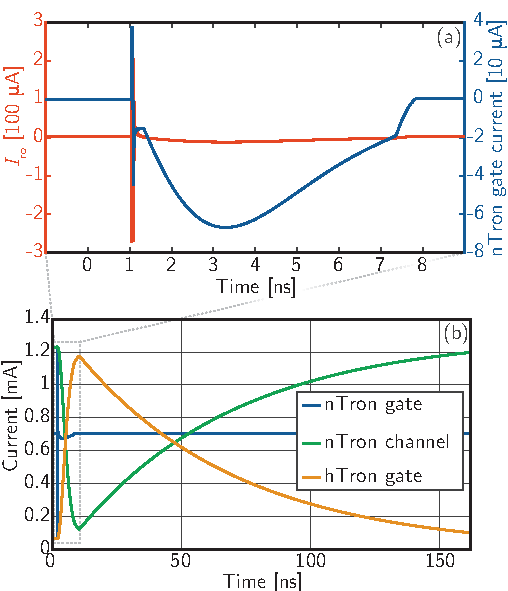
\includegraphics[width=8.6cm]{_transmitters_jjTriggersNTron_small.pdf}}
	\caption{\label{fig:transmitters_jjTriggersNTron}Time-domain simulations of the threshold detection event. (a) A fluxon from the threshold junction $J_{\mathrm{th}}$ switches $J_{\mathrm{ro}}$. The current diverted from $J_{\mathrm{ro}}$ to the gate of the nTron is plotted as a function of time. (b) The nTron source/drain current and the hTron gate current as a function of time following the threshold detection event. The simulation shown in Fig.\,\ref{fig:transmitters_jjTriggersNTron} was initiated with a DC pulse of 50\,mV into a DC-to-SFQ converter \cite{vatu1998,ka1999} that produced a fluxon. This fluxon propagated through a JTL before switching the relaxation-oscillator junction. This JTL is not essential for operation, and it adds negligible power consumption to the threshold detection event.}
\end{figure} 

The series of events shown in Fig.\,\ref{fig:transmitters_jjTriggersNTron} comprise the detection of neuronal threshold (which occurs when $J_{\mathrm{th}}$ switches), and the subsequent current amplification, beginning with the switching of $J_{\mathrm{ro}}$, and leading to the switching of the nTron. The 1.2\,mA current pulse coming from the nTron and driving the gate of the hTron has been shown in Sec.\,\ref{sec:hTron} to be sufficient to switch the hTron, resulting in a voltage pulse and light generation from the LED. The $L/r$ time constant in this simulation was 50\,ns, corresponding to 500 nH in series with the 10\,$\Omega$ of the hTron gate. Figure\,\ref{fig:transmitters_hTron_data_2}(b) shows this nTron time constant is sufficient to produce more than 3000 photons if the LED capacitance is 10\,fF and the LED efficiency is 1\%. Increasing the nTron inductance can extend the pulse duration and thereby produce more photons. With the material and device parameters used in this model of the nTron, 50\,ns recovery was sufficient to keep the nTron from latching, and shorter recovery times may be possible, depending on electro-thermal device engineering. As discussed in Sec.\,\ref{sec:hTron}, a square rather than exponential current pulse would have a significant impact on the light-production efficiency. Such operation may be achieved with cascaded hTrons in place of the nTron.

Having demonstrated threshold detection, current amplification, and voltage amplification, we have completed the description of the amplification chain of the neuronal transmitter circuit. We next discuss the efficiency of the amplifier chain.
	
\subsection{\label{sec:efficiency}Photon production efficiency}
%\input{transmitters_efficiency}
In Secs.\,\ref{sec:LED}-\ref{sec:detectingThreshold} we describe circuits capable of detecting threshold in the NT loop, amplifying the signal, and producing the voltage necessary to generate light from a semiconductor diode. We have calculated the energy consumed by each element of the amplifier chain when generating the number of photons necessary for neuronal communication in realistic networks. These networks will comprise a variety of neurons with a range of numbers of synapses. The number of out-directed synapses made by a neuron is referred to as the out-degree, $k_{\mathrm{out}}$. The number of photons that must be produced in a neuronal firing event depends on $k_{\mathrm{out}}$, and therefore so does the energy of a neuronal firing event, which we denote by $E_{\mathrm{out}}$.

\begin{figure}[t!]
	\centerline{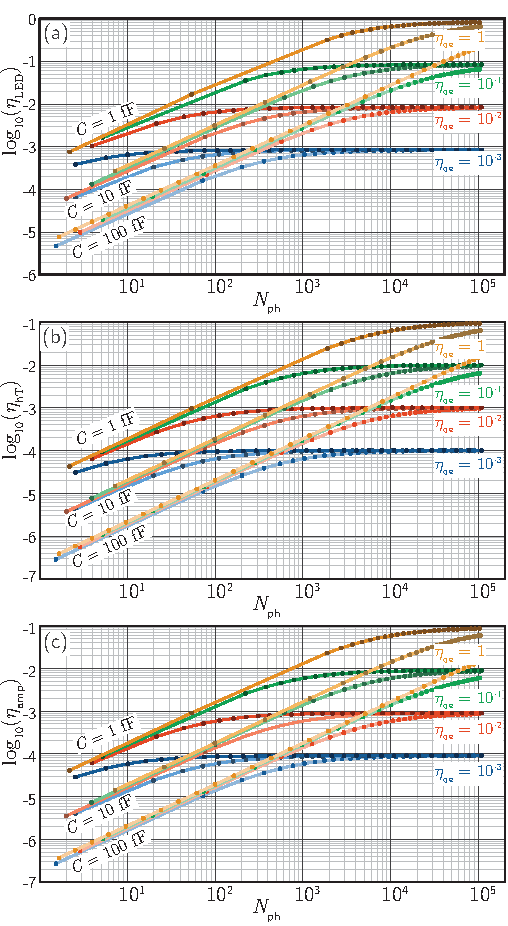
\includegraphics[width=8.6cm]{_transmitters_efficiency_small.pdf}}
	\caption{\label{fig:transmitters_efficiency}Efficiency of the photon production process as a function of the number of photons produced. (a) Efficiency of the LED. (b) Efficiency of the hTron. (c) Combined efficiency of the LED and hTron.}
\end{figure}
In an ideal case, a neuron could produce one photon per synaptic connection with unity production efficiency, the photons would reach their destination without loss, and they would be detected at the synapse with unity detection efficiency. In this case, we would have $E_{\mathrm{out}} = h\nu k_{\mathrm{out}}$. In an actual network implemented in hardware, waveguides will have propagation loss, and detectors will have efficiency less than unity. To account for these loss mechanisms, a neuron will produce a number of photons greater than one per synaptic connection. We refer to the number of photons produced per synaptic connection as $\zeta$. If $\zeta$ is too large, neurons are wasting power. If $\zeta$ is too small, communication will be unreliable. The synapses of Sec.\,\ref{sec:receiverCircuits} have the same response if they receive one or more photons. Therefore, the noise is not shot noise, as it would be if the synapse were attempting to detect the precise number of incident photons. The communication error can be calculated from the Poisson distribution. Given an average number of incident photons on a synapse due to an upstream neuronal firing event, we use the Poisson distribution to calculate the probability that a synapse will receive zero photons due to a neuronal firing event. If the average number of incident photons is five, the probability that the synapse will receive zero photons is less than 1\%. A neural system is likely to be able to tolerate this level of error \cite{stgo2005}. In the case of lossy waveguides with low-efficiency detectors, 3\,dB loss may be incurred between a neuron and a synaptic target. We thus consider $\zeta = 10$ to be a representative number to use in calculations of network power consumption.

In addition to propagation loss and detector inefficiency, the circuits described in this work are not entirely efficient at producing photons. The total energy consumed by the amplifier chain during a neuronal firing event is given by
\begin{equation}
\label{eq:energy}
E_{\mathrm{amp}}(N_{\mathrm{ph}}) = \zeta h \nu N_{\mathrm{ph}}/\eta_{\mathrm{amp}}(N_{\mathrm{ph}}),
\end{equation}
where $\eta_{\mathrm{amp}} = \eta_{\mathrm{LED}}\,\eta_{\mathrm{hT}}$. Note that $\eta_{\mathrm{hT}}$ includes all contributions from the nTron and the hTron. The Josephson circuits driving the nTron contribute negligible energy consumption. The calculations of Secs.\,\ref{sec:LED} and \ref{sec:hTron} provide us with numbers for $\eta_{\mathrm{LED}}$ and $\eta_{\mathrm{hT}}$ for several values of LED capacitance and internal quantum efficiency. These functions are plotted in Fig.\,\ref{fig:transmitters_efficiency}(a) and (b). Figure \ref{fig:transmitters_efficiency}(c) shows the total amplifier efficiency, $\eta_{\mathrm{amp}}$. We see that driving the hTron with the nTron (Fig.\,\ref{fig:transmitters_efficiency}(b)) dominates power consumption, yet the amount of time the hTron must be on is determined by the emitter capacitance and efficiency, and therefore emitter improvement is necessary for system improvement. The circuits can also be made more efficient with improved thermal design of the hTron (through phonon localization) and current pulse shaping into the hTron gate.

In practice, achieving small, waveguide-integrated LEDs with low capacitance should be possible. A simple parallel plate model indicates 1\,fF should be achievable, and 10\,fF should not be particularly challenging, even with wiring parasitics. In Fig.\,\ref{fig:transmitters_efficiency}, we consider values as poor as 100\,fF. The quantum efficiency of the device is harder to predict. Waveguide-integrated light-emitting diodes with efficiency near 0.01 have been demonstrated \cite{doro2017}, and low-temperature operation helps significantly in this regard. We expect quantum efficiency of 0.01 to be achievable at large scale, but in Fig.\,\ref{fig:transmitters_efficiency} we consider values as poor as $10^{-3}$. Considering an LED with 10 fF capacitance or less, if the LED efficiency is as poor $10^{-3}$, the total photon production efficiency of the amplifier chain is $\eta_{\mathrm{amp}} \approx 10^{-4}$ when more than 200 photons are produced. For calculating the power consumption of the networks described in Sec.\,\ref{sec:networks}, we use Eq.\,\ref{eq:energy} with $\zeta = 10$ and $\eta_{\mathrm{amp}} = 10^{-4}$.
			
\subsection{\label{sec:discussion_transmitterCircuits}Discussion Regarding Transmitter Circuits}
With the design of the transmitter portion of the circuit, the neuron model presented in this paper is complete. The full circuit is shown in Fig.\,\ref{fig:transmitters_fullCircuit}. The analysis presented here points to two conclusions. The first conclusion is that to produce photons with short pulses from the hTron, it is necessary to fabricate LEDs with low capacitance. Other integrated photonic applications find that capacitance dictates the scale at which light becomes advantageous \cite{mi2017}. The second conclusion is that the overall photon production efficiency is limited by the internal quantum efficiency of the LED when producing large numbers of photons. As argued in Sec.\,\ref{sec:introduction}, cognitive neural systems are likely to utilize some neurons with relatively small out-degree making only local connections as well as other neurons with high degree making local and long-range connections. The value of capacitance achievable by the LED will determine the lowest degree practical to implement with photonic connectivity.
\begin{figure*}[t!]
	\centerline{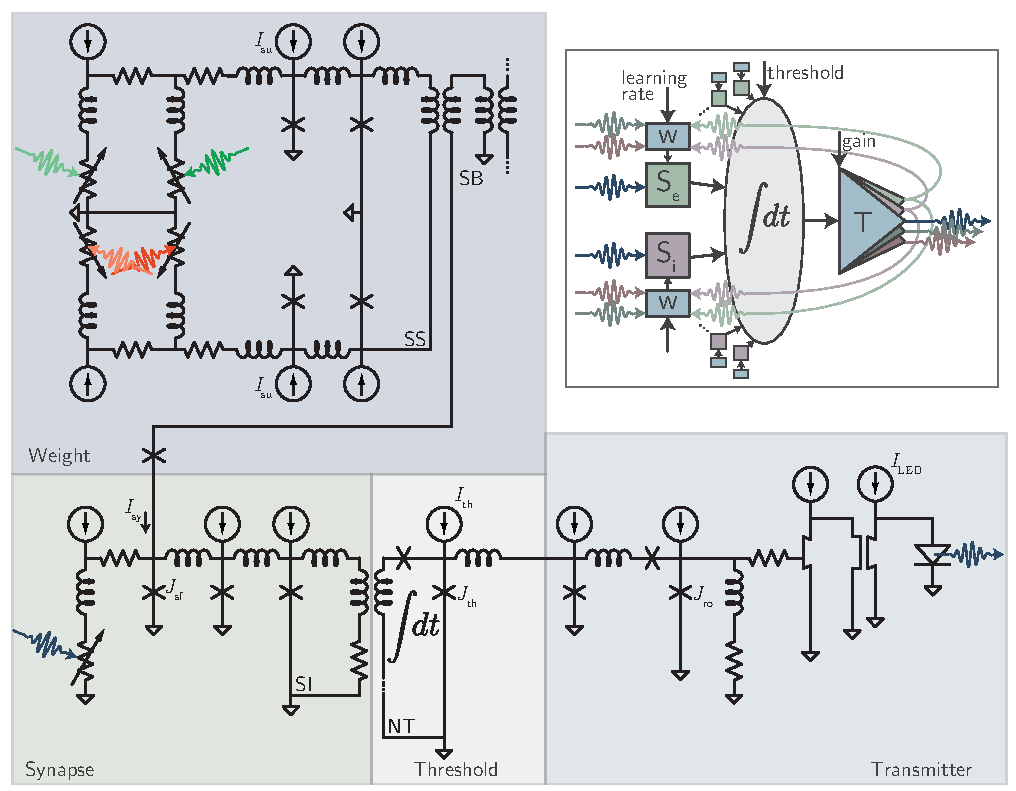
\includegraphics[width=17.2cm]{_transmitters_fullCircuit_small.pdf}}
	\caption{\label{fig:transmitters_fullCircuit}Circuit diagram of superconducting optoelectronic loop neuron. Large-scale neural systems will employ a wide variety of neurons with myriad structural and dynamical properties. The full potential of neural circuits based on superconducting optoelectronic hardware will only be realized with a long-term experimental and theoretical effort of a broad research community.}
\end{figure*}

While capacitance limits utility for low-degree operation, internal quantum efficiency determines system power consumption dominated by neurons with high degree. The maximum achievable quantum efficiency will depend on emitter design, materials employed, and fabrication optimization. The requirements for this approach to neural computing differ from the requirements of other integrated photonics applications. Emitters with carrier recombination times as long as 50\,ns, the same as the SPD recovery time, can be tolerated. For many integrated photonics applications, such a light source would be too slow. The ability to produce light at multiple frequencies may be advantageous, but spectral coherence is not required. Compound semiconductors have these spectral and temporal properties, and they can be integrated with silicon waveguides \cite{doro2017} with high efficiency, particularly at cryogenic temperature. Yet fabrication with compound semiconductors is more expensive and more difficult to scale than silicon. Cryogenic operation enables several types of silicon light sources \cite{da1989,shxu2007,buch2017}, which bring the advantage of simpler process integration. Whatever the material, sources providing incoherent pulses with 10,000 photons produced with efficiency of 10$^{-3}$ operating at 20\,MHz at 4.2\,K are sufficient to enable a massively scalable neural computing platform with connectivity comparable to the brain and thirty thousand times faster speed.

It may not be necessary to incorporate a light source at each neuron. Perhaps an architecture can be utilized with circulating light in waveguides that are tapped by a modulator during each neuronal firing event. Such a system would have the benefit of keeping light sources out of the cryostat and separate from superconducting circuits. In the case of shared off-chip light sources, the new challenges become to develop very low loss waveguides; compact, efficient modulators with low insertion loss that do not need to be tuned; and extensive fiber-to-chip coupling. Initial calculations indicate that such an approach is less efficient unless waveguides can be made with very low propagation loss, and modulators can be made with very low insertion loss. Yet device and system limits are far from understood. Amplifier circuits similar to those presented here may be useful when driving the modulators of such a system.

The synaptic receiver and synaptic weight update circuit in the form presented in Secs.\,\ref{sec:receiverCircuits} and \ref{sec:synapticPlasticity} utilize separate photons for synaptic firing and synaptic update. In this work, circuit operation culminates by producing light from a single LED, yet it may be desirable to implement transmitters that fire different LEDs for the different operations. This is one way that the power used for syanptic firing events can be decoupled from the power used for synaptic update events. If different colors are used for each of these operations, the same waveguide routing network can be employed for the three signals (synaptic firing, synaptic strengthening, and synaptic weakening), and the demultiplexers located at each downstream neuron can separate the signals and route them locally to the three synaptic ports. Similarly, the spike-timing-dependent plasticity circuit of Sec.\,\ref{sec:synapticPlasticity} requires not only photons from the pre-synaptic neurons, but also photons from the local, post-synaptic neuron. Two additional light sources may be useful at each neuron to be utilized locally for synaptic update. The schematic diagram in Fig.\,\ref{fig:general_schematic} shows these five light sources. While producing five light sources instead of just one adds hardware overhead, the light sources are extremely compact compared to the routing waveguides and inductors associated with the synapses. By utilizing independent light sources, it may be possible to reduce network area as well as power consumption.

The ability of a neuron to hold a refractory period is important for spiking operation. In the neuron under consideration, this is best achieved by cutting the bias to $J_{\mathrm{th}}$ upon neuronal firing. This makes it impossible for $J_{\mathrm{th}}$ the be driven above $I_{\mathrm{c}}$ and can be straightforwardly implemented with feedback from the output of the nTron or hTron.

In the schematic of Fig.\,\ref{fig:general_schematic}, we emphasize three main current biases that affect the operation of each neuron. A current bias into the synaptic update circuit of Sec.\,\ref{sec:synapticPlasticity} affects the learning rate. A current bias into the neuronal threshold loop affects the neuron threshold. And a current bias into the light emitter affects the number of photons produced in a neuronal firing event. With each of these currents fixed, the neurons and the network will have rich spatio-temporal dynamics. Yet a network with the ability to dynamically vary these currents will be capable of achieving further complexity over longer time periods. For example, with the learning rate current fixed, spike-timing-dependent plasticity occurs at a fixed rate. By changing this current, the network can make certain regions more adaptive at certain times, and it can make those regions maintain synaptic weights at other times. Similarly, with a fixed gain current into the transmitter, the neuron will address each of its downstream connections with a given probability. By changing the gain current, the number of photons produced in a neuronal firing event can be adjusted, and therefore the probability of reaching downstream connections can be tuned. Changing these bias currents is analogous to changing various neuromodulators in biological systems. The values of each of these neuromodulatory control currents can be modified with photonic or electronic signals set externally or based on internal network activity.

%---------------------------------------------
%networks
%---------------------------------------------	
\section{\label{sec:networks}Networks of Loop Neurons}
Neural computation depends critically on the structure of the network \cite{spto2000}. Whether the application of the network is for control, sensory processing, or cognition, efficient information processing requires the architecture to possess certain features. For example, in visual processing, local clusters of neurons must be differentiated to independently code for certain stimuli, yet the information from many such clusters must be combined at a larger scale to identify groupings of features and trends across a visual field \cite{haah2017}. Such differentiated local processing combined with broad integration repeats at multiple levels of hierarchy \cite{stsa2000,budr2004}. This hierarchical architecture leads to systems with fractal properties in space and time \cite{bu2006,busp2009}. Such an architecture balances differentiated, local information processing with efficient integration of information across the system \cite{to2004}. In this section, we begin to explore networks in which superconducting optoelectronic neurons can be connected to achieve the desired fractal network architectures.

We would like superconducting optoelectronic networks to meet several criteria: 1) physical instantiations must accomplish the networks in a manner that can be straightforwardly fabricated with conventional lithographic techniques; 2) the networks must achieve a hierarchical architecture that can be manufactured from the scale of a single die up to a 300 mm wafer; 3) for efficient information integration, systems at the die scale must contain hub nodes with thousands of synaptic connections, and at the scale of a wafer, which we would like to serve as a column in cortex, high-degree nodes with tens of thousands of edges must be possible \cite{sh2018_ICRC}; 4) considering these systems as modules, we extrapolate to neural systems at very large scales, where it must be possible to connect modules with dense local clustering into systems of billions of neurons for human-scale cognition; and 5) the power density of these networks must be low enough for cooling with $^4$He at 4.2\,K to be utilized. In this section we present SOEN designs satisfying these criteria.
	
\subsection{\label{sec:opticalCommunicationAndGraphMetrics}Optical Communication and Network Metrics}
%\input{networks_conceptualOverview}
Optical communication between neurons provides three major strengths. First, because photons are uncharged and massless, optical interconnects have no capacitance, resistance, or inductance, enabling massive fanout. Nodes with very high degree can be achieved without the need for multiplexed communication lines and signal arbitration \cite{lide2015}. Second, it is possible to send and receive single-photon signals, leading to communication with high energy efficiency \cite{mave2013}. Third, because light travels at the highest velocity in the universe, systems signaling with light can integrate the largest area of neurons with coherent oscillations. Yet devices based on optical signals have an important disadvantage: the device size is difficult to shrink below the wavelength of light. While superconducting optoelectronic neurons can make many connections, operate with high energy efficiency, and integrate a large area with coherent oscillations, the total number of neurons that can cooperate coherently depends on the total area of the system (limited by the speed of light) divided by the area of the individual neurons (limited by the wavelength of light). To begin to assess the potential of SOENs for near-term technological applications, we must analyze the types of systems that can be achieved on a single die, such as 1\,cm $\times$ 1\,cm. To assess the ultimate scaling potential of these networks when limited by light-speed communication, we must analyze what can be achieved within an area limited by the distance light can travel in the period of a network oscillation. We consider both these scales here.

Whether for near-term technological applications or long-term cognitive systems, the networks we wish to employ are likely to share several characteristics \cite{busp2009}. For cognitive systems large and small, differentiated processing balanced with information integration across spatial and temporal scales is crucial for performance \cite{tosp2003,to2004,to2008,bu2006,sp2010,base2011,haah2017}. Several network theory metrics can be employed to assess the fitness of a network for neural computing. We focus on three metrics relevant to differentiated processing and information integration. 

The first metric is clustering, which quantifies the prevalence of triangles in the network. Triangles refer to groups of three nodes connected by edges. High clustering enables information to be shared locally. To achieve differentiated information processing, we seek networks with a high degree of clustering compared to a random network with the same number of edges on the same vertex set. 

The second network metric is average path length. For a given network, we can calculate the shortest distance from every node to every other node. Averaging this distance over all pairs of nodes yields the average path length. To achieve information integration across spatial scales, the average path length should be nearly as small as the corresponding random network. High clustering with short path length characterize a small-world network \cite{wast1998}. 

The third network metric is the degree distribution. The degree of a node refers to the number of edges it forms with other nodes. In the present work, we consider two degree distributions: power-law and delta-function. For information integration across spatial scales with efficient wiring \cite{busp2012}, the degree distribution of the nodes in the network may follow a power law, thereby achieving a scale-free network \cite{baal1999}. Small-world, power-law networks have efficient communication, a balance of differentiation and integration, fractal properties of self-similarity across spatial scales, and are observed in many natural settings, including the networks of the brain \cite{egch2005}. We also consider structures closer to random networks, characterized by Gaussian degree distribution, which are optimized for short path lengths. Highly connected random networks with short path lengths are ideal for associative memories, such as hippocampus. We approximate the narrow Gaussian with a delta function, meaning all nodes of the network have the same degree. 

To achieve information integration across time, concepts of self-organized criticality \cite{bata1987,yara2017} are pertinent. In the temporal domain, differentiated local processing combined with large-scale information integration result in a power-law frequency distribution of transient synchronized oscillations \cite{budr2004,bu2006}. This $1/f$ behavior leads to fractal use of time as well as space, and gives rise to neuronal avalanches \cite{be2007} and criticality thought to be necessary for information integration and cognition \cite{be2007,kism2009,shya2009,rusp2011}. In the human brain, $1/f$ behavior is observed from 0.05\,Hz to 600\,Hz, spanning four orders of magnitude \cite{budr2004,bu2006}. For SOENs to achieve criticality, the devices and the network must support oscillations with frequencies obeying a power-law distribution \cite{bu2006} over several orders of magnitude. As we have argued, SOENs will support oscillations up to at least 20\,MHz, potentially spanning many more orders of magnitude that the brain. 

Here we consider specific networks with high clustering, short average path length, and power-law degree distribution that are suitable for differentiated processing combined with hierarchical information integration. We approximate the area and power consumption of such networks when implemented with superconducting optoelectronic hardware, and we anticipate the scaling of these networks when limited by light-speed communication. We focus here on micro-architecture at the level of neuron connectivity with the goal of identifying scaling laws for systems achievable in the near term. To develop a correspondence between the adjacency matrix of the network \cite{eskn2015} and the physical hardware that will perform the neural operations, we model the spatial extent of neurons and construct a routing scheme to calculate the area of waveguide interconnects (analogous to white matter in the brain).
	
\subsection{\label{sec:networkConstruction}Network Construction}
To achieve high clustering, short average path, and power-law degree distribution while setting ourselves up for straightforward, modular fabrication, we construct our adjacency matrix in a hierarchical manner, as shown schematically in Fig.\,\ref{fig:networks_schematic}. At the smallest network scale, neurons are tiled in a grid to form a local sector (Fig.\,\ref{fig:networks_schematic}(b)). Sectors can then be tiled to form regions. Regions can then be tiled to form modules. In the present work, we consider these three levels of hierarchy, but the algorithm for creating the adjacency matrix can be repeated indefinitely. 
\begin{figure}[t!]
	\centerline{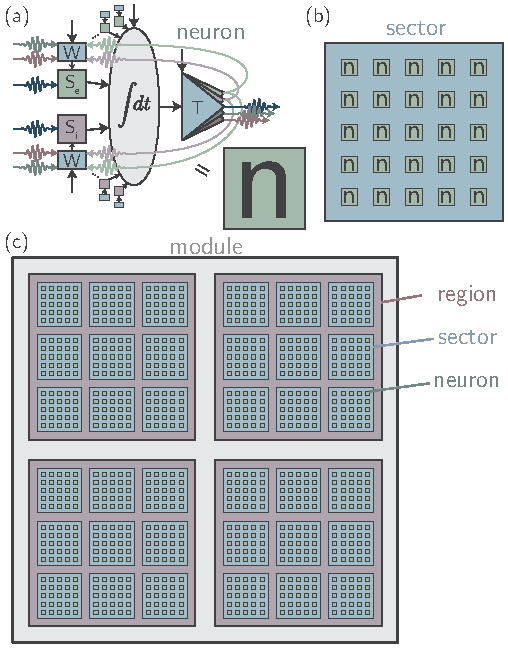
\includegraphics[width=8.6cm]{_networks_schematic_small.pdf}}
	\caption{\label{fig:networks_schematic}Schematic of networks under consideration. (a) Relating the neuron schematic used throughout this paper to the symbol used here. (b) Diagram of a sector of neurons. (c) Diagram of a module comprising multiple sectors and regions.}
\end{figure}
Networks constructed in accordance with the schematic of Fig.\,\ref{fig:networks_schematic}(c) with dense intra-sector connectivity, few connections between sectors within a region, and sparse connectivity across a module are modeled after the horizontal connections in mini-columns and columns within cortex \cite{mo1997,spto2000,brto2006,haah2017}. Feed-forward, vertical connections are likely to be achieved by stacking such networks, either through sequential processing or multi-die assemblies.

Networks with high clustering and average path length close to that of a random network can be constructed in many ways. Here we use a network growth algorithm. The concept is that the adjacency matrix of a local sector of neurons is formed by adding neurons one by one to the pool, establishing edges based on spatial location as well as the degree of the existing nodes. Such an algorithm introduces winner-take-more development, leading to a few nodes with very high degree, thereby extending the degree distribution to larger values. The next level of hierarchy can be generated by tiling the adjacency matrix of the sector along the diagonal of a larger adjacency matrix representing the region, and forming inter-sector connections in a manner that again depends on space and node degree. Networks of increasing scale can be achieved by repeating this procedure, thereby achieving the fractal, power-law degree distribution conducive to efficient information integration across the physical substrate of the network. The spatial dependence gives high clustering, which leads to functional differentiation. Reciprocal connection rules contribute to clustering as well as reentrant connections \cite{spto2000}, which give rise to transient temporal correlations that are necessary for information integration across time. The degree dependence of the growth algorithm gives rise to the long tail of the degree distribution, including nodes with high degree, which are advantageous for information integration across space. We have used this growth algorithm to generate a specific network adjacency matrix with 8100 nodes and 330,430 edges in the hierarchical configuration of Fig.\,\ref{fig:networks_schematic}(c). 

It is important to disambiguate two senses in which a network may have fractal spatial properties. We have been discussing the power-law degree distribution, which relates to a network that is scale-free in terms of connectivity. We can also consider the spatial scales across which connections are made. Rentian scaling quantifies fractal properties related to the number of connections made through various partitions of the network. This scaling relates the number of nodes within a topological partition, $n$, to the number of edges crossing the boundary of that partition, $e$ \cite{bagr2010}. If the relation between $e$ and $n$ follows the form $e\propto n^p$, the network shows fractal topology, and the Rent exponent, $p_T$, is given by $p_T = \mathrm{log}(e)/\mathrm{log}(n)$. The Rent exponent is related to the topological dimension, $D_T$, by $p_T \ge 1-\frac{1}{D_T}$. Consideration of Rentian scaling and topological dimension provide a means to assess a network's connectivity across various levels of hierarchy. 

In the present context, Rentian analysis provides one way to assess the potential for information integration across the physical space of the network. The larger the topological dimension, the more access nodes will have to distant members of the network. For the hierarchical network designed with the growth algorithm, we can approximate $p_T$ by considering the number of nodes and edges at each of the three levels of hierarchy. For the specific network under consideration, averaging over the neurons in a local sector, we find there are 17.1 edges into each neuron from other neurons within the sector. Considering a region, there are 17.8 edges into each neuron from other neurons within the region, but not in the same sector. And at the scale of the module there are 17.6 edges into each neuron from neurons in other regions. Based on this analysis, we calculate a Rentian exponent very close to unity. This gives a topological dimension of $D_T \rightarrow \infty$. This implies the network can integrate information up to infinite levels of hierarchy,which of course is not possible, as the network only comprises three levels of hierarchy. Networks with large topological dimension support self-organized criticality \cite{be2007,rusp2011}, which is advantageous for information integration in neural systems \cite{be2007,kism2009,shya2009,ch2010,rusp2011}. In networks from C. elegans to the human brain as well as in VLSI wiring, the Rentian exponent is closer to 0.75 \cite{bagr2010}. This analysis indicates that the network considered here has slightly more long-range connectivity than is necessary. The Rentian exponent can be adjusted within the growth algorithm by adjusting the number of connections made to higher levels of hierarchy.  
	
\subsection{\label{sec:physicalInstantiation}Physical Instantiation}
\begin{figure*}[t!]
	\centerline{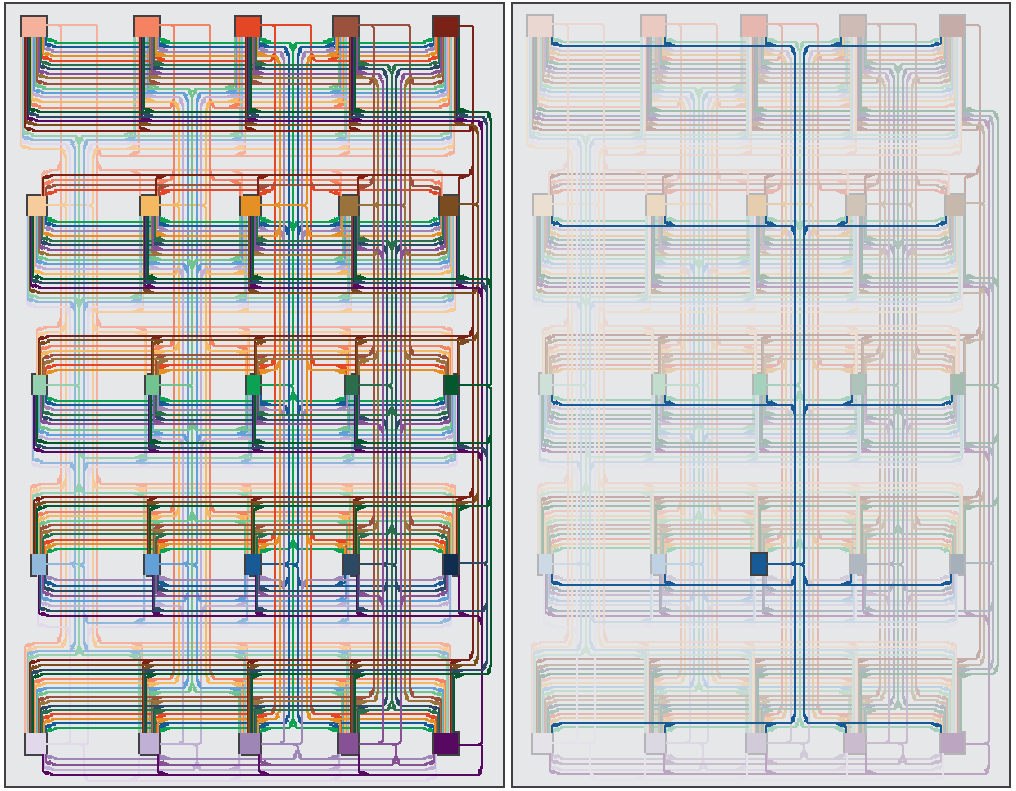
\includegraphics[width=17.2cm]{_networks_routingDiagram_small.pdf}}
	\caption{\label{fig:networks_routingDiagram}Row-column routing architecture in 5 $\times$ 5 sector showing all-to-all connections. The right panel highlights the connections from a single neuron.}
\end{figure*}
We seek estimates for physical aspects of SOENs, including size and power dissipation. We first introduce a plausible routing scenario for connecting the neurons in the network described in the previous section. 

\subsubsection{Passive waveguide routing}
To achieve the massive connectivity required of a neural system, each neuron must send its signals to many different destinations. To achieve this with optical signals in a controlled manner, multiple planes of dielectric waveguides \cite{chbu2017,chbu2018,sami2017} must be employed to keep waveguide crossing losses as low as possible and to reduce the area occupied by passive routing. We anticipate employing waveguide planes in pairs. Within each pair, one plane runs predominantly north-south, the other predominantly east-west. The vertical gap between waveguides in a pair is smaller than between the top waveguide in one pair and the bottom waveguide of the subsequent pair. The lowest pairs of waveguides will be used for the most local connections, with higher pairs for successively longer distances. Materials with lower index contrast may be used on higher planes to minimize loss in long-distance connections. In the context of the network discussed in Sec.\,\ref{sec:networkConstruction}, it is natural to use one pair of waveguide planes for intra-sector connections, a second pair for intra-regional connections, and a third pair for intra-modular connections.

In Fig.\,\ref{fig:networks_routingDiagram} we show a row-column routing scheme that connects all neurons in a sector to all other neurons in that sector. This approach to routing results in rows and columns densely packed with communication lines, analogous to the white matter of axons in biological neural systems. The connections from a single neuron are highlighted, and inter-planar couplers are drawn as pairs of triangles. We utilize row-column routing to minimize the number of inter-planar couplers required. The rules governing the routing are described in Appendix \ref{apx:sectorRouting}, which also discusses routing in feed-forward networks that are used in many machine-learning applications.

While we have shown Fig.\,\ref{fig:networks_routingDiagram} to depict neurons connected in a sector, the diagram can also be interpreted as showing sectors connected in a region or regions connected in a module. This fractal spatial property is a result of the hierarchical architecture we intend to employ for cognitive computing, and it is typical of networks characterized by high topological dimension. So far we have considered networks with three levels of hierarchy, but this fractal pattern can extend indefinitely. In the present context, we envision the row-column routing architecture extending beyond even the chip or wafer scale into multi-chip and multi-wafer assemblies with fiber optics forming dense white-matter connections between modules in three dimensions. 

\subsubsection{\label{sec:sizeOfNeurons}Size of neurons} 
The size of the neurons described in Secs.\,\ref{sec:receiverCircuits} - \ref{sec:transmitterCircuits}, when arranged in the networks described in Sec.\,\ref{sec:networkConstruction}, is calculated in Appendix \ref{apx:sectorRouting}. We use a spatial model of a superconducting optoelectronic neuron and routing waveguides shown in Fig.\,\ref{fig:networks_areaDiagram}(a). A schematic of how fabricated layers may be stacked is shown in Fig.\,\ref{fig:networks_areaDiagram}(b). 
\begin{figure}[t!]
	\centerline{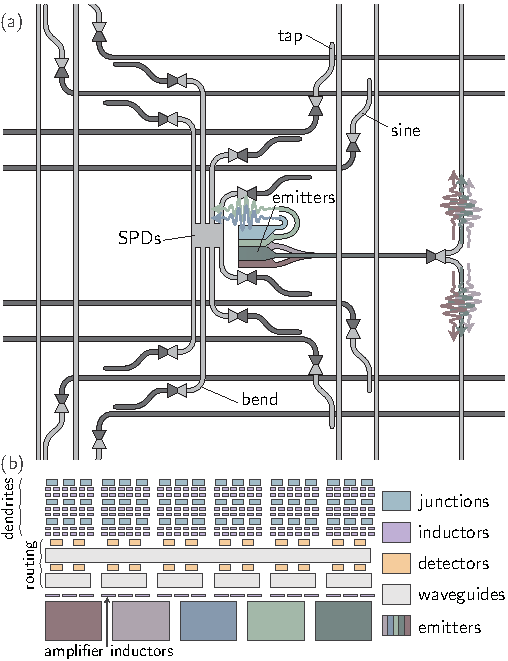
\includegraphics[width=8.6cm]{_networks_areaDiagram_small.pdf}}
	\caption{\label{fig:networks_areaDiagram}Schematic of physical instantiation of neuron. (a) Pictoral motivation for area calculation (details in Appendix \ref{apx:sectorRouting}). Five emitters are shown producing photons for various synaptic operations. (b) Schematic of the fabrication layer stack. There is one layer of emitters at the bottom. Above the emitters are the inductors necessary to drive the emitters. Next are repeating layers of dielectric waveguides, superconducting detectors, and superconducting inductors. Josephson junctions are patterned above the waveguides and superconducting wires.}
\end{figure} 
Applying the analysis of Appendix \ref{apx:sectorRouting} to the network of 8100 neurons discussed in Sec.\,\ref{sec:networkConstruction}, we calculate that the network will fit on a die 1\,cm $\times$ 1\,cm using a pair of waveguide planes for intra-sector routing, another pair for inter-sector routing within each region, and a third pair for inter-regional connectivity. 

We would like to approximate the size of networks with more neurons. The model informs us that the area of a neuron will follow a power law as a function of node degree. We show the area of a network as a function of the total number of neurons in the network in Fig.\,\ref{fig:networks_scaling}(a) for the cases of three pairs of waveguide planes and nine pairs of waveguide planes. In both cases, the degree distribution of the nodes takes the form $p(k) = Bk^{-\gamma}$ with $\gamma = 1.6$, where $p(k)dk$ is the probability of a node having degree between $k$ and $k+dk$. We find that by utilizing nine pairs of waveguide planes, we can accommodate an integrated system of one million neurons on a 300\,mm wafer. This network would comprise over 200 million complex synapses, as described in Sec.\,\ref{sec:synapticPlasticity}. Considering instead a network with delta function degree distribution (Fig.\,\ref{fig:networks_scaling}(b)), we find a network of 3000 neurons each with 300 synapses will occupy a 1\,cm $\times$ 1\,cm die. A 300\,mm wafer will support 40,000 neurons with 4000 connections per neuron. The number of synapses within a given area is similar for the power-law degree distribution and the delta function degree distribution. The main difference is the power-law degree distribution contains more neurons with fewer synapses and a few neurons with many synapses. Both network architectures are likely to be useful for certain types of information processing.

Appendix \ref{apx:sectorRouting} describes the calculation of the area of a neuron based on consideration of optical waveguides and single-photon detectors. From this area estimate, we can calculate the area available for the superconducting electronic components that contribute to the neuron, assuming they are patterned above the waveguides in repeating layer modules, as shown in Fig.\,\ref{fig:networks_areaDiagram}(b). The area available for superconducting inductors, mutual inductors, and Josephson junctions is given by the area of the node divided by the in-degree. This area is multiplied by the number of repeating layers utilized in the fabrication process. We find the area available for superconducting electronic components is at least 30\,\textmu m $\times$ 30\,\textmu m. A 1\,\textmu H inductor is on the larger end of what is likely to be utilized by the SI loop or SS loop. When constructed of a material such as MoSi with high kinetic inductance (180\,pH/$\square$) and patterned with 50\,nm lines, the area is 5\,\textmu m $\times$ 5\,\textmu m. This leaves plenty of area for multiple inductors and wiring. The mutual inductors required to couple the SI loop to the NI loop will be patterned with a different superconducting material separated from the high-kinetic inductance layer by an insulator. Mutual inductance of 100\,pH is desirable. Again, it is quite possible to fabricate a 100\,pH mutual inductor from two superconducting coils within this area. Each synapse also requires on the order of 10 JJs with $I_{\mathrm{c}}$ near 40\,\textmu A. These devices are approximately 1\,\textmu m $\times$ 1\,\textmu m, and will easily fit in the available area. Finally, the largest components of the neurons are likely to be the amplifiers that drive the light emitters and the mutual inductor coupling the neuronal integration loop to the neuronal thresholding loop. These devices are not required at every synapse, but rather only at each neuron. Therefore, area is not likely to be a problem. Passive photonic waveguides are likely to dictate the area, and they are limited by the wavelength of light.

We have mentioned in this paper that neurons based on similar JJ circuits, but using no optical components, could be created with much the same design as the neurons in Sec.\,\ref{sec:receiverCircuits} and synapses in Sec.\,\ref{sec:synapticPlasticity}. The purely electrical neurons would have difficulty achieving the fanout necessary for the networks discussed here. Nevertheless, the electrical neurons could potentially achieve $k\approx$\,20 with a more compact footprint, lower power dissipation, and higher speed. It may be advantageous to construct a hybrid network with nodes from $k = 2$ to $k = 20$ being purely electrical neurons with flux quanta playing the role of photons. We consider a network with power-law distribution wherein nodes with $k = 2$ to $k = 20$ are assumed to be electrical neurons, and nodes with $k > 20$ are assumed to be optical neruons. We perform an area calculation using modified forms of Eqns.\,\ref{eq:wCol} and \ref{eq:hRow} using physical dimensions appropriate to superconducting wiring rather than photonic waveguides. Whereas a network of just over one million optoelectronic neurons fit on a 300\,mm wafer, a network of 4 million total neurons can be achieved if we combine low-degree superconducting neurons with high-degree photonic neurons. This network would comprise over one billion synaptic connections. Such an architecture would extend the spatial power-law distribution to lower degree while extending the temporal power-law distribution to higher frequency. 
 \begin{figure}[t!]
	\centerline{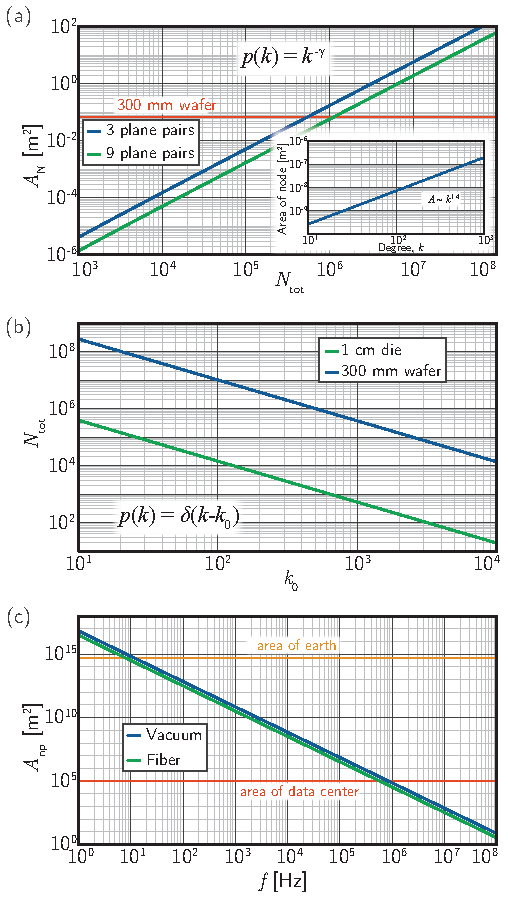
\includegraphics[width=8.6cm]{_networks_scaling_small.pdf}}
	\caption{\label{fig:networks_scaling}Scaling analysis. (a) Network with power-law degree distribution. Area as a function of total number of neurons for three and nine pairs of waveguide planes. The inset shows the area of a single node as a function of node degree when three routing planes are used. (b) Network with delta function degree distribution. The number of neurons that can fit on a 1\,cm $\times$ 1\,cm die and 300\,mm wafer as a function of node degree, $k_0$. (c) Area of the neuronal pool as a function of the frequency of oscillations for signals propagating in vacuum and fiber.}
\end{figure}

\subsubsection{\label{sec:neuronalPool}The neuronal pool}
In addition to comparing to the size of a die or a 300\,mm wafer, we must also consider the largest SOEN that can be established. This limit is not technological or economic in nature, but rather it is a physical limitation set by the velocity of communication. 

Consider two neurons separated by a distance $d$. At time $t_1$, neuron one produces a pulse. At time $t_2$, neuron two produces a pulse. We ask whether the pulse generated by neuron one may have contributed to the pulse by neuron two. In particular, we are interested in whether neuron one may drive neuron two to synchronize. For this consideration, the time scale we consider is the inverse of the frequency of oscillation, $T = 1/f$. Thus, if 
\begin{equation}
\label{eq:neuronalPool_diameter}
d \le \frac{v}{f},
\end{equation} 
neuron one can induce neuron two to synchronize with oscillations at frequency $f$. For the present discussion, we take the value of $d$ that saturates the inequality of Eq.\,\ref{eq:neuronalPool_diameter} to define the diameter of the neuronal pool. This result of the size of the coherent neuronal pool decreasing as the inverse of the frequency of synchronized oscillations \cite{lued1997} is consistent with observations from neuroscience \cite{stra1999} where the slow conduction velocity of axons is a severe limitation to the size of a synchronized network \cite{budr2004,bu2006,buwa2012}. 

Based on Eq.\,\ref{eq:neuronalPool_diameter}, we see the area of the neuronal pool scales as $A_p \propto (v/f)^2$. The number of neurons in the pool depends also on the size of the neurons. Here we consider spatial scaling in terms of the size of a synapse, because neurons many have any number of synapses, and therefore may span a wide range of sizes, whereas the size of synapses depend less on the degree of the neuron to which they are connected or the total size of the system in which they operate. We suppose the synapses in a network can be characterized by an average width, $w$. If we assume a network has connectivity predominantly in a plane (as is the case for mammalian cortex and as we expect from lithography on wafers), the area of a single synapse scales as $A_n \propto w^2$. For a given hardware platform sending signals at velocity $v$ to synapses of width $w$, the number of synapses within an neuronal pool with synchronized oscillations at frequency $f$ scales as $N_p \propto A_p/A_n \propto (v/fw)^2$. 

We wish to compare the number of synapses in the pool of two different hardware platforms oscillating at the same frequency, $f$. In particular, we wish to compare SOENs to the human brain. Denoting the two hardware platforms with superscripts, we find
\begin{equation}
\label{eq:neuronalPool_number}
\frac{N_p^{(\mathrm{soen})}}{N_p^{(\mathrm{brain})}} = \left(\frac{v^{(\mathrm{soen})}w^{(\mathrm{brain})}}{w^{(\mathrm{soen})}v^{(\mathrm{brain})}}\right)^2.
\end{equation}
A 300 mm wafer can support roughly $2\times 10^8$ superconducting optoelectronic synapses, giving $w^{(\mathrm{soen})} = 1.9\times10^{-5}$\,m. The area of the human cerebral cortex is 0.095\,m$^2$ \cite{scva2014}, and it contains $1.6\times 10^{10}$ neurons \cite{azca2009,he2009}. If we assume each neuron has, on average, $10^4$ synapses \cite{brsc1998}, this gives $w^{(\mathrm{brain})} = 2.4\times 10^{-8}$\,m. A biological synapse is 1000 times smaller than a superconducting optoelectronic synapse in width, and a million times smaller in area. The speed of signals in cortex is roughly 2\,m/s \cite{edve2004}. Axons with larger diameter can propagate signals above 100\,m/s, but for the dense connectivity of cortex, such large fibers cannot be supported. The speed of light is $3\times 10^8$\,m/s \cite{speedOfLight}. Thus, comparing SOENs to biological networks, we find $N_p^{(\mathrm{soen})}/N_p^{(\mathrm{brain})} \approx 10^{10}$. The neuronal pool enabled by light-speed communication can contain ten billion times the number of synapses as the pool enabled by ionic signal propagation along biological axons. Signaling at the speed of light brings a tremendous advantage in this regard, an advantage made more significant in networks spanning a volume rather than an area. This simple scaling analysis does not take into account factors that may be significant for very large systems, such as volume required for liquid helium flow for cooling or the volume of white matter occupied by optical fibers carrying signals between large modules. Suppose these factors introduce a quadratic error, and the correct scaling is the square root of this estimate. We would still be considering a system with 100,000 times the number of synapses as the human brain. Despite the coarse nature of this comparison, we include it here to emphasize a crucial point. Communication at the speed of light is likely to enable neural systems with many more neurons and synapses than the human brain even though photonic neurons and synapses are significantly larger than their biological counterparts.

It has been hypothesized that the conduction velocity of axons limits the size of biological neural systems, and that scaling of a single cognitive system much beyond the human cortex may not be possible with biological axon conduction velocities \cite{rido1994,bu2006}. Based on these scaling arguments, we expect the largest cognitive systems in the universe to communicate at the speed of light, enabling full utilization of each neuron's light cone. While other approaches to neural computing may utilize light for communication, it is unlikely other photonic neural devices will be significantly smaller than those presented here, as the optical wavelength imposes a practical spatial limit. In Fig.\,\ref{fig:networks_scaling}(c) we show the area of the neuronal pool as a function of oscillation frequency $f$ for a general neural system communicating at the speed of light. When oscillating at 1\,MHz, an area the size of a large data center ($10^5$\,m$^2$) can be coherently synchronized. When oscillating at 10\,Hz (near the $\theta$ and $\beta$ bands of the human cortex), an area the size of the surface of the earth can by coherently synchronized. Cognitive systems far beyond our comprehension may be possible with light-speed communication and single-photon efficiency.

\subsubsection{Power consumption}
In addition to the size of a SOEN, we must also consider its power consumption, which depends on the energy per synapse event, the degree distribution of the neurons, and the firing frequency distribution of the neurons. Analysis of power consumption in the networks under consideration is detailed in Appendix \ref{apx:power}. From that analysis, we find if we assume total photon production efficiency of $\eta_{\mathrm{tot}} = 10^{-4}$, the network of 8100 neurons will dissipate 1\,mW of device power, a trivial load for a modern cryogenic system. Including the power dissipated to establish bias currents, total on-chip power will be less than 10\,mW. The dominant power draw is the cryo cooler, and for this system it would require a few hundred watts.

For the system of one million neurons and 200 million synapses on a 300\,mm wafer, the total device power dissipation would be approximately 1\,W. This is the cooling power of a common Gifford-McMahon cryocooler with base temperature of 4.2\,K, drawing roughly 1\,kW. 

In addition to low total power, the power density of these systems is also quite small. For the case of the network on a wafer, the power density is 10\,W/m$^2$ if a poor total light-generation efficiency of $\eta_{\mathrm{tot}} = 10^{-4}$ is assumed. The heat produced can be straightforwardly removed, and immersion in a liquid helium bath will be excellent for this purpose \cite{ek2006}. This power density is far below the threshold for boiling liquid helium. Liquid helium is transparent at telecommunication wavelengths with an index of refraction very close to one. Thus, optical signals can be sent between neural modules in this environment without attenuation at the maximum speed allowed in the universe. Because the area of devices grows as a faster function of node degree than the power dissipation, cooling SOENs is possible in principle up to systems with size limited by the speed of light.

\subsection{\label{sec:discussion_networks}Discussion Regarding Networks of Loop Neurons}
We have argued that neural systems benefit from at least three network structural characteristics: clustering, short paths, and power-law scaling. We have utilized an algorithm to generate adjacency matrices with these characteristics that correspond to networks hierarchically arranged across spatial scales, and we have proposed that such networks could be implemented with superconducting optoelectronic hardware using 300\,mm lithographic technology. Networks with millions of neurons and hundreds of millions of synapses can be fabricated on a 300\,mm wafer. While Moore's Law has been sustained through feature size reduction, scaling of SOENs will be enabled by scaling the process up in terms of number of processed layers, lithographic field area, wafer size, and multi-wafer assemblies. Whereas economics has driven CMOS to bigger wafers, network scaling will drive SOENs to bigger wafers. Fortunately, feature sizes in all devices of this system are easily achievable with 190-nm lithography.

As described in Sec.\,\ref{sec:cognitiveSystems}, this work is motivated by the intention to develop artificial cognitive systems. We have investigated the utility of superconducting optoelectronics to achieve multiple neuronal functions with adaptation across a wide range of time scales, meeting many of the needs for relaxation oscillators in complex cognitive circuits. We have investigated the communication networks necessary to enable dense local clustering as well as long range connectivity for efficient communication across temporal and spatial scales. We have considered area and power consumption, and we find compelling evidence that this hardware platform has extraordinary potential to perform the functions underlying cognition. We think this work makes a strong case that a significant experimental effort to develop superconducting optoelectronic hardware is justified.

We are interested in systems with near-term feasibility. Considering the aforementioned network of 8100 neurons and 330,430 synapses, the network occupies 1\,cm $\times$ 1\,cm when processed with 3 pairs of waveguiding planes. Operating at 20\,MHz and possibly far beyond, the dynamical state space of this system would be extraordinarily complex and could provide a fascinating experimental setting for many subjects including self-organized criticality \cite{be2007,kism2009,shya2009,ch2010,rusp2011} in an artificial network approximating cortex. Such a neural module is also likely to offer significant technological opportunities in applications such as visual and auditory sensory processing, language recognition, and mechanical control.  

When combined with an artificial retina based on superconducting detectors, a powerful artificial vision system could result. A three-chip stack could accomplish this. One chip would serve as a retina, and the other two chips would serve as layers of visual cortex, arranged in a manner analogous to the columnar organization of the mammalian visual cortex \cite{mo1997}. Feed-forward communication is likely to make use of vertical optical links with light in a lower layer being sent vertically with a grating coupler and received by a single-photon detector at a neuron on a higher layer. Such a model, capturing the columnar, vertical flow of information between layers as well as the laminar, horizontal flow within layers \cite{lued1997,spto2000,brto2006}, has been shown to function well for object recognition in computer simulations \cite{haah2017}. Using visual systems as a testbed of SOEN hardware is beneficial because photon detectors are native to the hardware, and also because the visual system is the most studied system of the mammalian cortex. Investigation of binding in vision \cite{ro1999,tr1999,woca1999,vala2001,enfr2001,haah2017} can inform other neural computing systems including motor control systems, language processing, or other cognitive architectures.

Similar modules are also likely to tile well into larger networks. With a 10 $\times$ 10 grid of interconnected die, the system would contain as many neurons as a bumble bee, a creature observed to have advanced navigational skills \cite{chmi2014}; multimodal communication and learning \cite{alpe2016}; cognitive flexibility \cite{lope2017}; and emotions \cite{peba2016}. A 300 mm wafer would yield enough die for six of these small brains. Each system would comprise nearly a million neurons and over 33 million synapses with complex plasticity and metaplasticity. These neurons and synapses would operate up to thirty thousand times faster than any known living creature. Such a system would be readily accommodated by existing cryostats.  

If one chose to utilize an entire 300\,mm wafer for a single module, neurons with as many as ten thousand synapses could integrate the activity of networks with a million neurons. Such a structure would be analogous to a module in cortex, except for the significant increase in speed. Considering such modules as the building blocks of larger systems, stacks of wafers could be assembled with free-space and fiber coupling between. We can consider an interconnected stack of wafers as a column. An arrangement of columns could be interconnected to contain tens of billions of neurons, matching the number in the human neocortex \cite{brsc1998,he2009}. A SOEN with the same number of neurons as human cortex would occupy a volume less than two meters on a side. 

While it may be difficult to build systems larger than 10 billion neurons in the near term, such a system is not physically limited. Like the brain, such limits will be incurred due to the velocity of signal propagation. From Fig. \ref{fig:networks_scaling}(c) we know that networks as large as data centers can sustain coherent oscillations at 1\,MHz. Such a facility would house $10^8$ 300\,mm wafers if they were stacked 100 deep. This would result in 100 trillion neurons per data center across modules interconnected with another power-law distribution. 

Networks need not oscillate at 1\,MHz, and if they supported system-wide activity at 1\,kHz\textemdash faster than any oscillation of the human brain\textemdash the neuronal pool could occupy a significant fraction of the earth's surface and employ quintillions of neurons. We do not wish to cover earth in such devices, but asteroids provide ample, uncontroversial real estate. The materials for this hardware are abundant on M-type and S-type asteroids \cite{mufo2017,astra,bu1999,shcl2010,necl2014}. It appears possible for an asteroid belt to form the nodes and light to form the edges of a solar-system-scale intelligent network. Asteroids can be separated by billions of meters, so light-speed communication delays may be several seconds or longer. For cognitive systems oscillating up to 20\,MHz, such delays would cause individual modules to operate as separate cognitive systems, much like a society of humans. 

\section{Acknowledgements}
We thank Dr. Alexandra Artusio-Glimpse, Bryce Primavera, and Dr. Alexander Tait, for helpful conversations and insights.

\vspace{0.5em}
This is a contribution of NIST, an agency of the US government, not subject to copyright.
	
\newpage
\appendix
	
%---------------------------------
%receivers appendices
%---------------------------------
\section{\label{apx:circuitParameters}Parameters used in circuit simulations}
\subsection{Receiver circuits}
Unless otherwise specified, we take $I_{\mathrm{spd}} = 10$\,\textmu A, comparable to the switching current of MoSi \cite{veko2015} SPDs. Designs with lower $I_{\mathrm{spd}}$, as would be present in WSi nanowires \cite{mave2013}, or higher $I_{\mathrm{spd}}$, as would be present in NbN \cite{gook2001} or NbTiN \cite{miya2013} nanowires are also straightforward to achieve. The variable resistor of the SPD has zero resistance in the steady state, and it switches to a high-resistance state ($\approx$\,5\,k$\Omega$) temporarily ($\approx$\,200\,ps) upon absorption of a photon \cite{yake2007}. Typical values for the parameters in Fig.\,\ref{fig:receivers_circuitDiagrams}(a) are $L_{\mathrm{spd}} = 100$\,nH, $I_{\mathrm{spd}} = 10$\,\textmu A, $r_{\mathrm{spd}} = 2$\,$\Omega$, $I_{\mathrm{sy}} = 800$\,nA -  4\,\textmu A, $L_{\mathrm{sf}} = 200$\,pH, $I_{\mathrm{b}} = 7$\,\textmu A - 9\,\textmu A, $L_{\mathrm{si}} = 100$\,nH - 10\,\textmu H, and $M_{\mathrm{sy}} = 1$\,nH. The $I_{\mathrm{c}}$ of the JJs is chosen to be 10\,\textmu A in Sec.\,\ref{sec:receiverCircuits} to improve energy efficiency. In Appendix \ref{apx:power} we argue this is not necessary, and implementation with junctions of $I_c = 40$\,\textmu A or higher is probably a better design choice. The JJs used in simulations in this work have $\beta_c = 0.95$, where $\beta_c = 2eI_cCR^2/\hbar$, with $C$ the junction capacitance and $R$ the junction resistance in the RCSJ model \cite{vatu1998,ka1999}. The parameter $\beta_c$ corresponds to the junction damping (with $\beta_c = 1$ corresponding to critical damping), and for this study, we consider slightly over-damped junctions. Typical values for the transformer inductors in Fig.\,\ref{fig:receivers_circuitDiagrams}(b) are $L_{\mathrm{at1}} = 1$\,\textmu H, $L_{\mathrm{at2}} = 100$\,pH, and $L_{\mathrm{at3}} = 10$\,pH.

In all flux-storage loops, there is a trade-off between inductance and area. High-kinetic-inductance materials such as WSi have inductance per square as large as 250\,pH/$\square$. By patterning a nanowire of such a material in a meander geometry, we can produce an inductor with 10\,\textmu H in an area of 35\,\textmu m $\times$ 35\,\textmu m with a minimum feature size of 50\,nm. We argue in Sec.\,\ref{sec:networks} that these relatively large inductors are still compatible with scaling to neurons with 1000 synapses because the area of photonic routing is generally the limiting factor.

A JJ coupled to an inductive loop is often characterized by the parameter $\beta_L = 2\pi L I_c/\Phi_0$, which quantifies the amount of phase a loop can store. $\beta_L / 2\pi$ quantifies the number of flux quanta that can be stored. For the receiver circuits of Sec.\,\ref{sec:receiverCircuits}, $\beta_L/2\pi = 5\times10^2 - 5\times10^4$. For digital computing applications, $\beta_L/2\pi = 1.6$ is typical. There is also an area/inductance trade-off for the mutual inductor coupling each SI loop to the NI loop, and in the present work we choose 1\,nH for this mutual inductor.

When the value of $I_{\mathrm{b}}$ is 9\,\textmu A (Fig.\,\ref{fig:receivers_circuitDiagrams}(a)), current biases across $J_{\mathrm{sf}}$, $J_{\mathrm{jtl}}$, and $J_{\mathrm{si}}$ are 2.2\,\textmu A, 8.1\,\textmu A, and 8.8\,\textmu A, respectively, when the SPD is not firing and $I_{\mathrm{sy}} = 1$\,\textmu A. These numbers are 3.9\,\textmu A, 8.3\,\textmu A, and 8.8\,\textmu A when $I_{\mathrm{sy}} = 3$\,\textmu A. Of these three junctions, only $J_{\mathrm{jtl}}$ is not embedded in a high-inductance loop, making it the most susceptible to noise. This value of $I_{\mathrm{b}}$ has been chosen as a compromise between flux storage capacity of the SI loop and imperviousness to noise. Based on the analysis of Ref.\,\onlinecite{sesc2016}, we calculate the effective temperature, $\tilde{T} = 2\pi k_{\mathrm{B}} T/\Phi_0 I_c$, and inductance parameter, $\lambda = \Phi_0/2\pi LI_c$, where $L$ is the total inductance of the loop. For the junctions under consideration with $I_c = 10$\,\textmu A at 4.2\,K, $\tilde{T} = 0.0176$. The Josephson inductance of the junctions at zero bias is 33\,pH, giving a total loop inductance of 266 pH and an inductance parameter of $\lambda = 0.124$. With these values of $\tilde{T}$ and $\lambda$, the analysis of Ref.\,\onlinecite{sesc2016} informs us that biasing $J_{\mathrm{jtl}}$ with 8.1\,\textmu A is below the switching current of 9\,\textmu A at 4.2\,K. If an application requires further noise reduction, very similar circuit operation can be achieved by applying $I_{\mathrm{b}} = 7$\,\textmu A, provided the range of synaptic biases is shifted to 2\,\textmu A $< I_{\mathrm{sy}} < 4$\,\textmu A. With $I_{\mathrm{b}} = 7$\,\textmu A, the bias across $J_{\mathrm{jtl}}$ is 6.6\,\textmu A when $I_{\mathrm{sy}} = 4$\,\textmu A.

It may be the case that for different applications or during different periods of learning and operation, different amounts of noise are tolerable or even desirable. Changing between $I_{\mathrm{b}} = 7$\,\textmu A and $I_{\mathrm{b}} = 9$\,\textmu A can be done dynamically during operation to modify the stochasticity of the synaptic transducer with no required hardware compensation. Thus, one can utilize or suppress noise at will depending on the context \cite{vrso1996,vora2005,stgo2005}. Further, because synaptic firing events will produce tens to hundreds of fluxons, thermal switching events resulting in the addition of a single fluxon to the SI loop may be inconsequential. The complexity of the effects of noise on the operation of this circuit merit further investigation.

Regarding the two-photon coincidence detector of Fig.\,\ref{fig:receivers_coincidence}, to emulate the physical rebiasing behavior and critical current of the SPDs, JJs with 11\,\textmu A $I_{\mathrm{c}}$ were placed in series with each SPD. The main panel shows simulations of a circuit with $L_{\mathrm{spd}}/r_{\mathrm{spd}} = 1$\,\textmu H$/2\Omega = 500$\,ns, and the inset shows simulations of a circuit with $L_{\mathrm{spd}}/r_{\mathrm{spd}} = 1$\,\textmu H/20\,$\Omega$ = 50\,ns. The circuit of Fig.\,\ref{fig:receivers_coincidence} has been designed with 40\,\textmu A $I_{\mathrm{c}}$ JJs. Similar performance can be achieved with the 10\,\textmu A junctions used in the circuit of Figs.\,\ref{fig:receivers_schematic}(b) and \ref{fig:receivers_circuitDiagrams}. Here, $I_{\mathrm{b}} = 38$\,\textmu A. 

\subsection{Synaptic plasticity circuits}
The memory cell of Fig. \ref{fig:synapticPlasticity_binaryCircuit} has been designed with the following circuit parameters. $I_{\mathrm{ss}}^{\mathrm{b1}} = 38$\,\textmu A, $I_{\mathrm{ss}}^{\mathrm{b2}} = 20$\,\textmu A, $L_{\mathrm{ss}} = 90$\,pH. The four inductors comprising the two mutual inductors are labeled $L_1-L_4$ from left to right. Their values are $L_1=L_2=45$\,pH, $L_3=L_4=18$\,pH. $J_{\mathrm{su}} = 40$\,\textmu A, and $I_1 = 12$\,\textmu A. The junction $J_{\mathrm{sf}}$ with $I_{\mathrm{c}}$ of 10\,\textmu A is embedded in the SB loop. 

The memory cell of Fig. \ref{fig:synapticPlasticity_supervisedCircuit} has been designed with the following circuit parameters. The inductors comprising the DC-to-SFQ converter are, from left to right, $L_1 = 80$\,pH, $L_2 = 60$\,pH, $L_3 = 300$\,pH. The bias to the DC-to-SFQ converter is $I_{\mathrm{DC}} = 73$\,\textmu A. The drive current pulses are $I_{+} = 10$\,\textmu A with 100\,ps rise and fall time and 1 ns duration. The two biases to the SS loop are each $I_{\mathrm{ss}}^{\mathrm{b}} = 34$\,\textmu A. The mutual inductor parameters between the SS loop and the SB loop and from the SB loop to $I_1$ are, from left to right $L_1 = 18$\,pH, $L_2 = 190$\,pH, $L_3 = 18$\,pH, $L_4 = 18$\,pH, and $I_1 = 27$\,\textmu A. With $L_{\mathrm{ss}} = 20$\,nH, $\Delta I_{\mathrm{ss}} = 103$\,nA per pulse, and $\Delta I_{\mathrm{sy}} = 25$\,nA per pulse. The SS loop can store $-4.94$\,\textmu A $< I_{\mathrm{ss}} < 4.96$\,\textmu A.

All JJs in the synaptic plasticity circuits have $I_c = 40$\,\textmu A. In contrast to the synaptic receiver circuits of Sec.\,\ref{sec:receiverCircuits} where JJs with $I_c = 10$\,\textmu A were used, these JJs do not switch with every synaptic firing event, and consequently, using lower $I_{\mathrm{c}}$ for power minimization is less important. Using $I_c = 40$\,\textmu A leads to circuits with wider operating margins and ease of fabrication. We argue in Appendix \ref{apx:power} that using JJs with $I_c = 40$\,\textmu A for the circuits of Sec.\,\ref{sec:receiverCircuits} would also be satisfactory.

To achieve the desired Hebbian operation with the circuit of Fig.\,\ref{fig:synapticPlasticity_Hebbian_1}(a), several considerations are pertinent. When SPD$_1$ detects a photon, it needs to direct current predominantly to $I_2$, and not to $I_3$. When SPD$_2$ detects a photon, it needs to direct current predominantly to $I_3$, and not to $I_1$. These considerations inform us that we should choose $L_2 \ll L_3$ and $L_3 \ll L_1$. We choose $L_2 = 12.5$\,nH for this study. Such a small SPD may have reduced detection efficiency, but the inefficiency is tolerable for this purpose, because synaptic update will occur only rarely to optimize memory retention \cite{fuab2007,lide2015}. We then choose $L_3 = 125$ nH, and $L_1 = 1.25$\,\textmu H. The choices for $r_1$ and $r_2$ are made to achieve the desired temporal behavior. The $L/r$ time constants must be long enough to ensure the SPDs do not latch. Beyond this, they can be chosen to achieve the desired learning performance. We choose $\tau_1 = 50$ ns and $\tau_2 = 5$\,ns to facilitate WRSpice analysis, but longer time constants may be necessary in practice. In Fig.\,\ref{fig:synapticPlasticity_Hebbian_1}(a), $I_{\mathrm{spd}} = 10$\,\textmu A. The bias to the synaptic storage junction is 38\,\textmu A. All corresponding circuit parameters are the same for Fig.\,\ref{fig:synapticPlasticity_stdp}(a).

\subsection{LED driven by hTron}
The equations of motion for the circuit of Fig.\,\ref{fig:transmitters_LED_circuit} are
\begin{equation}
\label{eq:ledDrivenByHTron_equationOfMotion01}
\frac{dI_1}{dt} = \frac{1}{L}\left[V_2+r_{\mathrm{LED}}+I_{\mathrm{LED}}-(r_{\mathrm{LED}}+r_{\mathrm{hT}})I_1\right];
\end{equation}
\begin{equation}
\label{eq:ledDrivenByHTron_equationOfMotion02}
\frac{dV_2}{dt} = \frac{1}{C}[I_{\mathrm{LED}}-I_1-I_{pn}(V_2)].
\end{equation} 
In these equations, $I_{pn}$ is an analytical function which describes the LED's DC $I-V$ characteristic. It is given by \cite{stba2006}
\begin{equation}
\label{eq:ledDrivenByHTron_ledModel}
\begin{split}
I_{pn} = & eA\left[ (D_p/L_p)p_n + (D_n/L_n)n_p \right] \\
& \times\left[ e^{eV/k_BT} - 1 \right].
\end{split}
\end{equation}
The parameters that enter this equation are as follows. The number of acceptors, $N_a = 5\times 10^{19}$\,cm$^{-3}$. The number of donors, $N_d = 5\times 10^{19}$\,cm$^{-3}$. The intrinsic carrier density, $n_i = 1.5\times 10^{10}$\,cm$^{-3}$. The number of holes on the $n$ side of junction, $p_n = n_i^2/N_d$. The number of electrons on $p$ side of junction, $n_p = n_i^2/N_a$. The electron minority carrier lifetime, $\tau_{np} = 40$\,ns. The hole minority carrier lifetime, $\tau_{pn} = 40$\,ns. The mobility of holes on $p$ side, $\mu_{pp} = 10^{-2}$\,m$^2$/V$\cdot$s. The mobility of holes on $n$ side, $\mu_{pn}= 10^{-2}$ m$^2$/V$\cdot$s. The mobility of electrons on $n$ side, $\mu_{nn} =  2.5\times10^{-2}$\,m$^2$/V$\cdot$s. The mobility of electrons on $p$ side, $\mu_{np} = 2.5\times 10^{-2}$\,m$^2$/V$\cdot$s. The hole diffusion coefficient, $D_p = (k_BT/e)\mu_{pn}$. The electron diffusion coefficient, $D_n = (k_BT/e)\mu_{np}$. The hole diffusion length, $L_p = \sqrt{D_p\tau_{pn}}$. The electron diffusion length, $L_n = \sqrt{D_n\tau_{np}}$. $T = 300$\,K is the temperature of operation. While we plan to operate these circuits at 4.2\,K, our measurements indicate the model captures the operation well at low temperature, and the model is more stable with this room-temperature value. To approximate the capacitance we have assumed the length of the junction is $5$\,\textmu m, the height of the junction is 200\,nm, the intrinsic region is 100 nm, and $\epsilon = 12$ for the semiconductor. This gives $C = 1$\,fF, which is the smallest value we have considered. Fringe fields and wiring parasitics will likely increase this value. We have considered capacitance as large as 100\,fF to ensure our estimates are conservative.

\subsection{hTron circuit model}
The equations of motion for the circuit in Fig. \ref{fig:transmitters_hTron_circuit}(b) are given by
\begin{equation}
\label{eq:hTron_eq01}
\frac{dT_1}{dt} = \frac{Q}{C_1} + \frac{T_2-T_1}{R_1C_1};
\end{equation}
\begin{equation}
\label{eq:hTron_eq02}
\frac{dT_2}{dt} = \frac{T_1-T_2}{R_1C_2} + \frac{T_3-T_2}{R_2C_2};
\end{equation}
\begin{equation}
\label{eq:hTron_eq03}
\frac{dT_3}{dt} = \frac{T_2-T_3}{R_2C_3} + \frac{T_4-T_3}{R_3C_3};
\end{equation}
\begin{equation}
\label{eq:hTron_eq04}
\frac{dT_4}{dt} = \frac{T_3-T_4}{R_3C_4} + \frac{T_g-T_4}{R_4C_4}.
\end{equation}
In the calculations presented in Fig.\,\ref{fig:transmitters_hTron_data_1} and \ref{fig:transmitters_hTron_data_2}, $Q = I^2r$ where $I = 1.2$\,mA is the current through the gate of the hTron, and $r = 10$\,$\Omega$ is the resistance of the hTron gate. Thus, $Q = 14.4$\,\textmu W.

To produce the plots shown in Fig.\,\ref{fig:transmitters_hTron_data_1} and \ref{fig:transmitters_hTron_data_2}, we model the heater layer as a 10\,nm-thick film of Al. The upper spacer is modeled as a 10 nm-thick film of a-Si, and the lower spacer is modeled as a 50 nm-thick film of SiO$_2$. For the material parameters, the following values are used. The density of Al was taken to be 2700\,kg/m$^3$, and the thermal conductivity was taken to be 30\,W/m$\cdot$K. The density of a-Si was taken to be 2285\,kg/m$^3$, and the thermal conductivity was taken to be 0.01\,W/m$\cdot$K \cite{zipi2006}. The density of SiO$_2$ was taken to be 2650\,kg/m$^3$ and the thermal conductivity was taken to be 0.01\,W/m$\cdot$K. The temperature-dependent specific heat of Al and SiO$_2$ were taken from Ref.\,\onlinecite{du2015}. 

Regarding the superconductor, we anticipate using MoSi for this purpose due to its resistivity in the normal state, its critical current density, and its critical temperature. In a film of 8 nm thickness, the sheet resistance in the normal state is 300 $\Omega/\square$. A wire of 100\,nm width can sustain 16\,\textmu A critical current. A length of 2000 squares achieves 800\,k$\Omega$. A meander of 2000 squares of a wire of 100\,nm width and 50\,nm gap fits in a square of $5.4$\,\textmu m $\times$ 5.4\,\textmu m. At this thickness, $T_{\mathrm{c}} = 6.2$\,K. A device held at 4.2\,K must only be raised by 2\,K to switch to the normal state. The temperature-dependent specific heat of MoSi was taken from Ref.\,\onlinecite{lasa1988}, and the thermal conductivity was taken to be 1\,W/m$\cdot$K.

Of the material parameters, the values of thermal conductivity are the most uncertain. From Ref.\,\onlinecite{zepo1971} we know the thermal conductivity of quartz and silica differ from one another by orders of magnitude at low temperature, and we expect the value of thermal conductivity to depend significantly on the specific material and film deposition method used in fabrication. For functional hTrons fabricated with SiO$_2$ spacer layers and operating between 1 and 5 K, it has been observed \cite{mc2018} that 18\,nW/\textmu m$^2$ is required to switch the hTron. When using the value of 0.01 W/m$\cdot$K for the thermal conductivity of the spacer layers, we arrive at a power density of 494\,nW/\textmu m$^2$ needed to elevate the structure above $T_{\mathrm{c}}$, a factor of 27 higher than the measured value. We therefore suspect hTrons can be more efficient than the present model would predict, but further empirical investigation is required to determine the limits of hTron efficiency. The model of Eqs. \ref{eq:hTron_eq01}-\ref{eq:hTron_eq04} neglects phonon reflection at material interfaces. This effect may be responsible for the discrepancy between the model and measurements. Utilizing phonon reflection or phononic crystals in design may further increase the efficiency of the device.

\subsection{Parameters used in threshold circuit}
%\input{transmitters_appendix_roParameters}
The $I_c$ of the JJs in the JTL in Fig.\,\ref{fig:transmitters_schematic}(a) is 250\,\textmu m, and the inductors are 2.1\,pH. The $I_c$ of the JJ just before the relaxation oscillator junction is 280\,\textmu m, and the $I_c$ of the relaxation oscillator junction is the same. The relaxation oscillator is biased with 140\,\textmu A. The value of $L_1 = 200$\,pH . The value of $r_1 = 2.76$\,$\Omega$. The value of $r_2 = 3$\,$\Omega$.

\section{\label{sec:appendix_energy}Energy of a synaptic firing event}
In the receiver circuit explored in this work, each fluxon produced by a synaptic firing event switches three JJs. When combined with the synaptic update circuit, a fourth JJ is necessary to act as a buffer between the synaptic update circuit and the synaptic firing circuit. Each switching operation dissipates energy $E_{J} = I_{\mathrm{c}} \Phi_{0}$. The total energy dissipated during a synaptic firing event can be minimized by reducing the number of junctions and by reducing their $I_{\mathrm{c}}$, but power dissipation will likely be dominated by light production (unless the light emitters can be made extremely efficient), so reducing the number of junctions or their $I_{\mathrm{c}}$s is not likely to be necessary from an energy perspective. 

The minimum $I_{\mathrm{c}}$ that can be used is determined by noise considerations. For this analysis, we compare the Josephson coupling energy, $I_{\mathrm{c}}\Phi_0/2\pi$, to $k_B T$ with $T = 4.2$\,K \cite{lise1991}. This informs us that the thermal-equivalent junction critical current is 176\,nA. For digital electronics wherein errors are intolerable, most systems employ JJs with $I_{\mathrm{c}} > 40$\,\textmu A. Neuromorphic circuits are resilient to errors and leverage noise \cite{vrso1996,vora2005,stgo2005}. These circuits can therefore operate with lower $I_{\mathrm{c}}$. In the present work, the circuit of Fig.\,\ref{fig:receivers_circuitDiagrams}(a) is designed with all three JJs having $I_{\mathrm{c}} = 10$\,\textmu A ($I_{\mathrm{c}}\Phi_0/2\pi > 50 k_B T$), giving a switching energy ($I_{\mathrm{c}}\Phi_0$) of $E_{J} = 21$\,zJ.

The energy of a synaptic firing event is due to rebiasing of the SPD, $E_{\mathrm{spd}} = L_{\mathrm{spd}}I_{\mathrm{spd}}^2/2$, as well as the energy dissipated by the junctions, $E_{\mathrm{JJ}} = 4I_{\mathrm{c}}\Phi_0$. The factor of four comes from the fact that the synaptic firing circuit has four JJs. If we assume the SPD is an out-and-back nanowire integrated with a waveguide \cite{spga2011,pesc2012,feka2015,shbu2017b} with 60\,\textmu m total length, 150\,nm width, and 180\,pH/$\square$, $E_{\mathrm{spd}} = 4$\,aJ. For a synaptic firing event with weak synaptic efficacy (33 fluxons), $E_{\mathrm{JJ}} = 2.7$\,aJ. For a synaptic firing event with strong synaptic efficacy (497 fluxons), $E_{\mathrm{JJ}} = 41$\,aJ. Operation with a weak synaptic weight could be engineered to produce zero fluxons, and a strong synaptic weight one fluxon, thereby reducing the analog transducer to a digital element and achieving the limit of energy efficiency of this part of the neural system. This is likely not necessary, as energy consumption is dominated by the production of photons by the transmitter circuit.
	
%---------------------------------
%networks appendices
%---------------------------------
\section{\label{apx:sectorRouting}Waveguide routing}
Minimization of wiring is an NP-complete problem, and we make no attempt to solve it in the present context with the constraints particular to SOEN hardware. Instead we develop a practical all-to-all routing scheme and arrive at wiring diagrams by pruning the complete set of connections down to those corresponding to the adjacency matrix of the network under consideration. This solution is likely not optimal, yet it accomplishes the goal of achieving integrated photonic connections between neurons represented by the relevant adjacency matrix. The routing scheme under consideration is shown schematically in Figs.\,\ref{fig:networks_routingDiagram} and \ref{fig:networks_areaDiagram}.

To route the waveguides connecting each neuron to all other neurons within a local sector, we begin with the center node. Light is assumed to exit the node to the east, and it branches into north-running and south-running waveguides on the upper waveguide plane. Each of these waveguides splits east and west at each row to send light to the neurons in that row. Inter-planar couplers \cite{chbu2017} are shown as pairs of triangles in Fig. \ref{fig:networks_routingDiagram}. Using these couplers, light is routed to the lower plane for east-west routing. It is routed back to the upper plane before entering the SPDs at each neuron. Interplanar transistions are required to mitigate losses due to waveguide crossings. Although intraplanar crossings can be used sparingly, their loss is high enough that they cannot be the exclusive means of crossing waveguides \cite{lish2014}. 

Connections from the central node to all other nodes are established in this manner. Next, a similar approach is taken for the node just north of the central node. Within the central routing column, each subsequent node has two waveguides running north-south. One is to the east of the center node's main north-south waveguide, and one is to the west. Such an approach adds a factor of two to the width of columns, but avoids intra-plane crossings. A better solution is likely possible. At each point where a waveguide must branch, a power tap evanescently couples the appropriate fraction of light to achieve the desired optical signal at all destinations \cite{chbu2018}. The objective is to couple as close to one photon as possible to each neuron while avoiding intolerable communication errors. In the power calculation presented in Sec. \ref{sec:physicalInstantiation}, we assume ten photons are produced for each synaptic connection, and reception of one or more photons will trigger a synaptic firing event. 

Routing proceeds by establishing the connections from each node up the center column followed by connections from each node below the center node down to the bottom of the center column. As each new row or column waveguide is added, it is placed outside the existing waveguides, leading to dense ribbons of waveguides in the rows and columns, as shown in Fig. \ref{fig:networks_routingDiagram}. To calculate the width of a column, we define the term
\begin{equation}
\label{eq:a}
\begin{split}
a & = w_{\mathrm{wg}}+g_{\mathrm{tap}}+h_{\mathrm{sine}} \\
& +(w_{\mathrm{wg}}+w_{\mathrm{IPC}})/2.
\end{split}
\end{equation}
Within this model, we calculate the width of a routing column as
\begin{equation}
\label{eq:wCol}
\begin{split}
w_{\mathrm{col}} &= 2 n_{\mathrm{row}}(a+g_{\mathrm{wg}})+2r_{\mathrm{bend}},
\end{split}
\end{equation}
and the height of a routing row as
\begin{equation}
\label{eq:hRow}
\begin{split}
h_{\mathrm{row}} &= n_{\mathrm{N}}\left[a+n_{\mathrm{spd}}(w_{\mathrm{wg}}+g_{\mathrm{wg}})\right]+2r_{\mathrm{bend}}.
\end{split}
\end{equation}
In these expressions, $n_{\mathrm{row}}$ is the number of rows in a sector, $g_{\mathrm{tap}}$ is the gap of an evanescent tap, $h_{\mathrm{sine}}$ is the height of sine bend for a power tap, $w_{\mathrm{wg}}$ is the width of a waveguide, $w_{\mathrm{IPC}}$ is the width of an inter-planar coupler, $g_{\mathrm{wg}}$ is the gap between two waveguides sufficient to avoid cross talk, $r_{\mathrm{bend}}$ is the radius of a routing bend, $n_{\mathrm{N}}$ is the number of neurons in a sector, and $n_{\mathrm{spd}}$ is the number of SPDs associated with each synapse. We take $n_{\mathrm{spd}}=3$ in this analysis to account for synaptic firing, Hebbian, and anti-Hebbian synaptic update signals from pre-synaptic neurons. Two SPDs receiving photons from the local, post-synaptic neuron are also required, but they do not need to be accessed via the same routing waveguides, and it is assumed these detectors can be patterned either below or above the routing infrastructure. 

The expressions in Eqs.\,\ref{eq:wCol} and \ref{eq:hRow} approximate the dimensions of routing channels for sectors with all-to-all connectivity, but in practice, connectivity will be much more sparse. To account for the sparsity, we multiply the width of Eq.\,\ref{eq:wCol} by $k_{\mathrm{out}}/n_{\mathrm{N}}$ and the height of \ref{eq:hRow} by a factor $k_{\mathrm{in}}/n_{\mathrm{N}}$ when calculating the contribution to the sector area by a neuron with out degree $k_{\mathrm{out}}$ and in degree $k_{\mathrm{in}}$. These in and out degrees refer to the degree calculated using only the adjacency matrix of the sector. That is, only connections which originate and terminate within a sector are accounted for in this part of the analysis. Distant connections are accounted for below.

The expressions in Eqs.\,\ref{eq:wCol} and \ref{eq:hRow} account for the area consumed by routing waveguides, but the contribution to total sector area due to the area of the neurons must also be included. We approximate the size of a neuron with
\begin{equation}
\label{eq:hNeuron}
h_{\mathrm{neuron}} = 2L_{\mathrm{spd}},
\end{equation}
and
\begin{equation}
\label{eq:wNeuron}
\begin{split}
w_{\mathrm{neuron}} &= k_{\mathrm{in}}(w_{\mathrm{wg}}+g_{\mathrm{wg}})\\
&+\frac{3}{2}(L_{\mathrm{tap}}+L_{\mathrm{sine}}+L_{\mathrm{DeMux}}+L_{\mathrm{IPC}}+r_{\mathrm{bend}}).
\end{split}
\end{equation}
In these expressions, $k_{\mathrm{in}}$ is the in-degree of the neuron, $L_{\mathrm{tap}}$ is the length of an average evanescent power tap, $L_{\mathrm{sine}}$ is the length of a sine in a power tap, $L_{\mathrm{DeMux}}$ is the length of a de-multiplexer used to separate the photons for synaptic firing, Hebbian, and anti-Hebbian update. While it is not necessary to use different colors for these different operations, it may be advantageous so the different operations can be turned on and off independently. If multiple colors are used, the de-multiplexer is likely to be a frequency-dependent evanescent coupler. $L_{\mathrm{IPC}}$ is the length of an inter-planar coupler.

To calculate the area of a sector, the areas occupied by routing and by neurons are summed, and the result is divided by the number of pairs of waveguide planes used in the fabrication process. Once the area of a sector has been calculated, we need to consider the area consumed by routing between sectors to form regions and between regions to form a module. For these calculations, the expression of Eqs.\,\ref{eq:wCol} and \ref{eq:hRow} are used, except $n_{\mathrm{row}}$ refers to the number of rows of neurons in the region (which is the number in a sector times the number of rows of sectors in the region), and $n_{\mathrm{N}}$ refers to the number of neurons in the region. The in and out degrees used now refer to connections originating in one sector of the region and terminating in a different sector of the same region. When calculating the area of a region, the area of the neurons is not added, as all inter-sector synapses are assumed to be above the intra-sector synapses on higher waveguide planes. This simplification can be made if the number of synapses resulting from intra-sector connections is equal to or less than intra-regional and intra-modular connections. This corresponds to a Rentian exponent less than one. For the case of the growth model network with 8100 neurons, the average number of intra-sector connections is 17.1. The average number of intra-regional connections is 17.8. The average number of intra-modular connections is 17.6. For the random network, these numbers are 0.4, 9.8, and 91.9, respectively. Routing and area analysis of the random network requires a different approach.

For the network of 8100 neurons considered in Sec.\,\ref{sec:networkConstruction}, there are three levels of hierarchy: sectors, regions, and the total module. The analysis of the area of routing waveguides in the module is nearly identical to the analysis of the regions with the appropriate substitutions of $n_{\mathrm{row}}$, $n_{\mathrm{N}}$, $k_{\mathrm{in}}$, and $k_{\mathrm{out}}$.

The size of the neurons and routing depend on the number of connections made by each neuron. Using the above expressions for the contribution of a neuron to the total area, we can calculate $A_n(k)$, the area of a neuron with degree $k$. Here we assume $k_{\mathrm{in}} = k_{\mathrm{out}} = k$. For the specific case of the network of 8100 neurons, we can explicitly calculate this area for each neuron because the adjacency matrix is known. In a general case, we can calculate the total area of a general network if the number of neurons and their degree distribution, $p(k)$, is specified. The total area of the network is given by
\begin{equation}
\label{eq:networkArea}
A_{\mathrm{N}} = N_{\mathrm{tot}}\int_{k_{\mathrm{min}}}^{k_{\mathrm{max}}}A_n(k)p(k)dk.
\end{equation}
For the analysis presented in Fig.\,\ref{fig:networks_scaling}(a), we use this expression to calculate the total network area, and we obtain $A_n(k)$ by fitting the data from the network of 8100 neurons to a power-law. From this fit, we find $A_n(k)\propto k^{1.4}$. To generate Fig.\,\ref{fig:networks_scaling}(a), we assume the in-degree and out-degree are the same. 

\begin{figure}[t!]
	\centerline{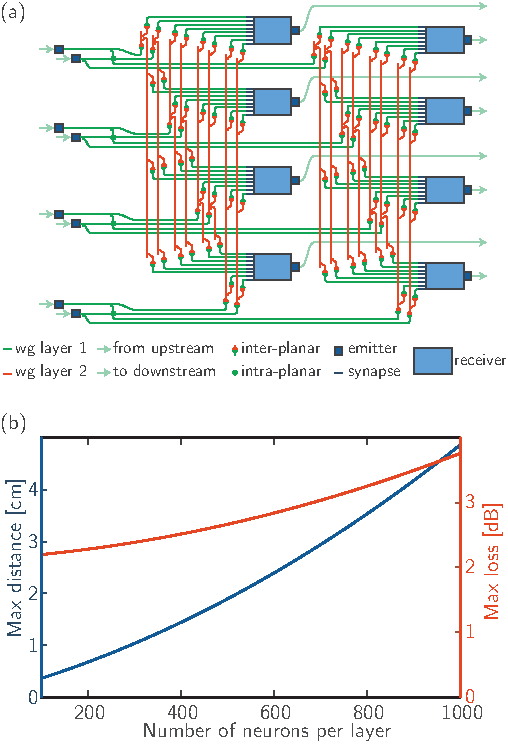
\includegraphics[width=8.6cm]{_networks_feedForward_small.pdf}}
	\caption{\label{fig:networks_feedForward}Routing for a feed-forward network. (a) Routing diagram. (b) Propagation distance and propagation loss as a function of the number of neurons per network layer.}
\end{figure}
The following parameters have been used in these calculations. The width of a waveguide, $w_{\mathrm{wg}} = 500$\,nm. The gap between waveguides, $g_{\mathrm{wg}} = 1$\,\textmu m. The height of a sine bend, $h_{\mathrm{sine}} = 1$\,\textmu m. The length of a sine bend is the same. The gap of an evanescent power tap, $g_{\mathrm{tap}}= 500$ nm. The length of a power tap, $L_{\mathrm{tap}} = 5$\,\textmu m. The length of an inter-planar coupler, $L_{\mathrm{IPC}} = 36$\,\textmu m. The width of an inter-planar coupler, $w_{\mathrm{IPC}} = 4$\,\textmu m. The length of an SPD, $L_{\mathrm{SPD}} = 10$\,\textmu m. The radius of a routing bend, $r_{\mathrm{bend}} = 2$\,\textmu m. The length of a de-multiplexer, $L_{\mathrm{DeMux}} = 5$\,\textmu m.
These parameters are intended to model silicon passive photonic components. For longer-distance connections, silicon nitride waveguides may be preferable due to the lower index contrast and therefore lower loss. The area of silicon nitride passive waveguides is roughly twice that of silicon.  

While the sector comprising a square array of nodes shown in Fig.\,\ref{fig:networks_routingDiagram} works well for the growth algorithm leading to power-law degree distribution, many applications leverage feed-forward networks that are very wide with only a few layers but all-to-all connectivity from one layer to the next. A routing diagram for such a network is shown in Fig.\,\ref{fig:networks_feedForward}. Here we again use pairs of waveguide planes for north-south and east-west routing. A similar spatial analysis as that represented by Eqs.\,\ref{eq:a} - \ref{eq:wNeuron} has been conducted. Figure \ref{fig:networks_feedForward}(b) shows the spatial scaling and loss as a function of the number of neurons in a network layer for a process employing 12 waveguide planes to form two layers of a feed-forward network. The maximum distance refers to the row-column propagation distance from a neuron at the bottom of one network layer to the top of an adjacent layer. It is assumed waveguides have 0.2 dB/cm propagation loss \cite{ch2018}. For 1000 neurons per layer, the system would fit on a chip 2.5\,cm $\times$ 2.5\,m.

\section{\label{apx:power}Network power consumption}	
For this analysis we model the energy to produce a photon as $E = h\nu/\eta_{\mathrm{tot}}$, where $h$ is Planck's constant, $\nu$ is the frequency of light (250\,THz if the emitters of Ref.\,\onlinecite{buch2017} are employed), and $\eta_{\mathrm{tot}}$ is an efficiency factor that takes into account all energy used by the thresholding junction, the superconducting amplifiers, and the light emitter. From Sec.\,\ref{sec:transmitterCircuits} we take $\eta_{\mathrm{amp}} = 10^{-4}$. Because power consumption is dominated by the amplifiers, we let $\eta_{\mathrm{amp}}\rightarrow\eta_{\mathrm{tot}}\rightarrow\eta$. The energy of a neuronal firing event is given by $E_{\mathrm{out}} = \zeta h \nu k_{\mathrm{out}}/\eta$, where $\zeta$ is the number of photons produced for each synaptic connection. In principle, this can be as low as one, but such low photon numbers would make communication noisy and unreliable. $\zeta = 10$ is likely to be a safe operating point, as described in Sec.\,\ref{sec:efficiency}. To calculate the total energy per neuronal firing event, we also need to sum the energy of all the synaptic firing events that led to the neuronal firing event. This energy is given by $E_{\mathrm{in}} = \chi n_{\mathrm{fq}} I_c \Phi_0 k_{\mathrm{in}}$ where $n_{\mathrm{fq}}$ is the number of fluxons generated in a synaptic firing event (taken to be 245), and $\chi$ is the fraction of synapses that must fire to drive the neuron to threshold. We assume $\chi = 1/3$ as an overestimate, given that $N_{\mathrm{sy}}^{-1/2}$ is observed in biological systems \cite{vrso1996,vora2005}. To simplify analysis, let us take $k_{\mathrm{in}} = k_{\mathrm{out}} = k$. The total energy of a neuronal firing event is thus
\begin{equation}
\label{eq:neuronalFiringEvent}
E(k) = (\zeta h \nu/\eta + \chi n_{\mathrm{fq}} I_{\mathrm{c}} \Phi_0) k\equiv E_0 k.
\end{equation}
The two contributions to Eq.\,\ref{eq:neuronalFiringEvent} are due to generation of photons during a neuronal firing event ($\zeta h \nu/\eta$), and generation of fluxons during a synaptic firing event ($\chi n_{\mathrm{fq}} I_{\mathrm{c}} \Phi_0$). These two terms are plotted independently in Fig.\,\ref{fig:networks_contributionsToEnergy}. We see the photon production efficiency, $\eta$, must be very high (\,$>0.2$) for the photonic contribution to be less than the fluxonic contribution. Based on this analysis, we conclude that the choice to use junctions with 10\,\textmu A $I_{\mathrm{c}}$ for the synaptic receivers of Sec.\,\ref{sec:receiverCircuits} was probably misguided, and it may be the case that all the circuits of Secs.\,\ref{sec:receiverCircuits} and \ref{sec:synapticPlasticity} can be produced with junctions of 40\,\textmu A $I_{\mathrm{c}}$. 
\begin{figure}[t!]
	\centerline{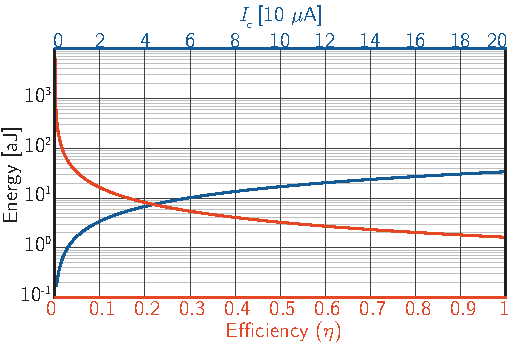
\includegraphics[width=8.6cm]{_networks_contributionsToEnergy_small.pdf}}
	\caption{\label{fig:networks_contributionsToEnergy}Photonic and electronic contributions to power. The red trace is the term $\zeta h \nu/\eta$, and the blue trace is the term $\chi n_{\mathrm{fq}} I_{\mathrm{c}} \Phi_0$.}
\end{figure}

The power dissipated by a neuron is given by the energy per neural firing event multiplied by the number of neural firing events per unit time, 
\begin{equation}
\label{eq:neuronPower}
P_{\mathrm{n}}(k,f) = E(k)f, 
\end{equation}
where the subscript $\mathrm{n}$ denotes the power of a single neuron as opposed to the total power of the network. 

We assume the network is characterized by a power-law degree distribution of the form
\begin{equation}
\label{eq:degreeProbability}
p(k) = B_1 k^{-\gamma},
\end{equation} 
meaning the probability that a node from the network chosen at random will have degree between $k$ and $k+dk$ is $p(k)dk$. We further assume the network is characterized by a power-law frequency distribution of the form
\begin{equation}
\label{eq:frequencyProbability}
p(f) = B_2 f^{-\mu},
\end{equation}
meaning that, during a period of observation, a node chosen at random from the network will be observed to spike with frequency between $f$ and $f+df$ is given by $p(f)df$. Incorporating these probability distributions, and assuming there are $N_{\mathrm{tot}}$ nodes in the network, the total network power consumption is given by
\begin{equation}
\label{eq:networkAverageTotalPower}
P_{\mathrm{N}} = N_{\mathrm{tot}}\int_{f_{\mathrm{min}}}^{f_{\mathrm{max}}} \int_{k_{\mathrm{min}}}^{k_{\mathrm{max}}} P_{\mathrm{n}}(k,f)p(k)p(f) dk df, 
\end{equation}
and the power density is $P_{\mathrm{N}}/A_{\mathrm{N}}$, where $A_{\mathrm{N}}$ is the total area of the network.

Considering first the spatial term of Eq.\,\ref{eq:networkAverageTotalPower}, we see that 
\begin{equation}
\label{eq:networkPower_spatialConsideration1}
P_{\mathrm{N}} \propto \int_{k_{\mathrm{min}}}^{k_{\mathrm{max}}} k^{-(\gamma-1)}dk, 
\end{equation}
whereas
\begin{equation}
\label{eq:networkPower_spatialConsideration2}
A_{\mathrm{N}} \propto \int_{k_{\mathrm{min}}}^{k_{\mathrm{max}}} k^{-(\gamma-1.4)}dk. 
\end{equation}
The exponent of 1.4 is explained in Appendix \ref{apx:sectorRouting}. Because the integrand of $A_{\mathrm{N}}$ decays more slowly with $k$ than the integrand of $P_{\mathrm{N}}$, power density will decrease as a function of network size, and will therefore never limit scaling. The exponents $\gamma$ and $\mu$ can also be chosen to adjust power density.

Considering the frequency term of Eq.\,\ref{eq:networkAverageTotalPower}, we see that 
\begin{equation}
\label{eq:networkPower_frequencyConsideration1}
P_{\mathrm{N}} \propto \int_{f_{\mathrm{min}}}^{f_{\mathrm{max}}} f^{-(\mu-1)}df. 
\end{equation}
The integrand in Eq.\,\ref{eq:networkPower_frequencyConsideration1} is the power spectral density of the network, 
\begin{equation}
\label{eq:networkPower_frequencyConsideration2}
P_{\mathrm{N}}(f) \propto f^{-(\mu-1)}. 
\end{equation}
If the exponent in the frequency power-law distribution (Eq.\,\ref{eq:frequencyProbability}) is $\mu = 2$, the network-averaged power spectrum of Eq. \ref{eq:networkPower_frequencyConsideration2} takes the $1/f$ form observed in cortical networks \cite{budr2004}, believed to be significant for cognition \cite{bu2006}, and known to be related to self-organized criticality and fractal objects \cite{be2007,bata1987,yara2017}. In the hardware platform under consideration, $\mu$ can be adjusted through the threshold bias currents as well as the light-emitter gain bias currents, thus providing a means to investigate network operation as a function of power spectral density.

Using Eq.\,\ref{eq:networkAverageTotalPower} to calculate the power consumption of the network of 8100 neurons, and assuming $f_{\mathrm{min}} = 100$\,Hz and $f_{\mathrm{max}} = 20$\,MHz, we find the network will consume 2\,mW. A network of 1 million neurons on a 300\,mm wafer will consume 2\,W. To calculate these numbers, we have assumed $\gamma = 1.4$ and $\mu  = 2$.

\bibliographystyle{unsrt}
\bibliography{loop_neurons}

\end{document}
